\documentclass[tcc]{ic}

\usepackage{bbm}
\usepackage{indentfirst}
\usepackage{lscape}
\usetikzlibrary{decorations}
\usetikzlibrary{shapes.symbols}
\usetikzlibrary{fit,positioning,arrows.meta}%RNN
\usetikzlibrary{shapes.arrows}
\usepackage{tikz}
\usetikzlibrary{matrix,chains,positioning,decorations.pathreplacing,arrows}
\usepackage{icomma}
\usepackage{smartdiagram}
\usepackage{microtype}
\usepackage{psfrag}
\usepackage{float}
\usepackage{verbatim}
\usepackage{tikz, pgfplots}
\usepackage{rotating}
\usepackage{rotfloat}
\usepackage[list-final-separator={ e }, range-phrase={ até }]{siunitx} %Para formatar datas e outros campos numéricos.
\usepackage{placeins} %Força Tabela/Figura ficar abaixo do texto.
\usepgfplotslibrary{fillbetween}
\usepackage{graphicx}
\usepackage{colortbl}
\usepackage{scalefnt}
\usepackage{chngpage}



\newenvironment{demonst} 
               {\noindent \textit{\textbf{Demonstração.}}~ } %begin demonst
               {\hfill\rule{2mm}{2mm} \vspace{\parskip} } %end demonst

\newtheorem{definicao}{Definição}[section]
\newtheorem{teorema}{Teorema}[section]
\newtheorem{lema}{Lema}
\newtheorem{corolario}{Corolário}
\newtheorem{proposicao}{Proposição}

\pgfplotsset{compat=1.7}

%ZIPF
\pgfmathdeclarefunction{gauss}{3}{%
\pgfmathparse{1/(#3*sqrt(2*pi))*exp(-((#1-#2)^2)/(2*#3^2))}%
}

%RNN
\tikzset{neuron/.style={shape=circle, minimum size=1.25cm, 
  inner sep=0, draw, font=\small}, io/.style={neuron, fill=gray!20}}

%======================================================%
%=========== Informações do documento PDF =============%
%======================================================%
\hypersetup{
colorlinks = {true},
linktocpage = {false},
plainpages = {false},
linkcolor = {Blue},
citecolor = {Blue},
urlcolor = {Red},
unicode = {true},
pdftitle ={Redes de Coautoria da Base SciELO: Avaliação da Colaboração Científica por Medidas de Centralidade de Redes Complexas},
pdfauthor = {Vitor Luiz Pereira Ribeiro},
pdfsubject = {Disserta\c c\~ao de Mestrado},
pdfkeywords={Bibliometria, Redes de Coautoria, Medidas de Centralidade},
pdfcreator = {LaTeX2e},
pdffitwindow = {false},
pdfstartview = {FitH},
pdftoolbar = {true},
pdfpagemode = {UseOutlines},
pdfview = {XYZ null null null}
}

%======================================================%
%================ CAPA DA DISSERTAÇÃO =================%
%======================================================%
\titulo{Redes de Coautoria da Base SciELO: Avaliação da Colaboração Científica por Medidas de Centralidade de Redes Complexas}

\autor{Vitor Luiz Pereira Ribeiro}{vitor.ribeiro@laccan.ufal.br}{}

\orientador{Dr. Alejandro C.\ Frery}{http://sites.google.com/site/acfrery/}{Instituto de Computação}{Universidade Federal de Alagoas}

\examinador{Dr. Osvaldo Anibal Rosso}{oarosso@gmail.com}{Instituto ou Departamento}{Instituto de Física \\ Universidade Federal de Alagoas}

\examinadorTres{Dr. Leonardo Melo de Medeiros}{}{Instituto ou Departamento}{Instituto Federal de Alagoas}

%\examinadorQuatro{Examinador 4}{ex4@email.com}{Instituto ou Departamento}{Universidade do Examinador 4}

\dataMesAno{Julho}{2019}

\begin{document}

\selectlanguage{portuguese}

\capa


%======================================================%
%======================= RESUMO =======================%
%======================================================%
\begin{resumo}
\noindent 

Na área de bibliometria, estudos vêm sendo realizados para mensurar quantitativa e qualitativamente a evolução da produção do conhecimento científico. Nesta direção, as redes de coautoria é uma das formas de indicar a interação entre autores, pelo esforço colaborativo entre pessoas, instituições e países para a geração e publicação de um trabalho científico. Este trabalho busca a propositura de uma análise investigativa a partir de base de dados de indexação de artigos científico SciELO, utilizando para tal, propriedades e métricas da teoria dos grafos e redes complexas, tais como \textit{degree centrality, betweeness centrality e closeness centrality}, propondo uma avaliação da rede global de coautoria das Universidades Federais do Brasil e da rede local, definida como vértice focal a Universidade Federal de Alagoas, para série temporal de 2008 à 2017 nas áreas de \textit{Health Sciences} - Ciências da Saúde, \textit{Agricultural Science} - Ciências Agrárias, \textit{Exact and Earth Sciences} - Ciências Exatas e da Terra. Este trabalhou baseou-se em uma metodologia que consistiu nas etapas: a) definição da rede, b) tratamento de dados, c) determinação das características estruturais, d) inspeção visual. Os resultados foram gerados numérica e graficamente, permitindo avaliações e interpretações do comportamento das redes estudadas com base nas medidas de centralidade utilizadas neste trabalho.

\vspace{1em}

\noindent
{\bf Palavras-chave}: Bibliometria, Redes de Coautoria, Medidas de Centralidade.
\end{resumo}

%======================================================%
%====================== ABSTRACT ======================%
%======================================================%
\selectlanguage{english}
\begin{abstract}
\noindent 

In bibliometrics field, studies have been carried out to quantitatively and qualitatively measure the evolution of the production of scientific knowledge. In this direction, co-authorship networks is one way of indicating the interaction between authors, through the collaborative effort between people, institutions and countries for the production and publication of a scientific work. This work seeks the proposition of an investigative analysis based on the index database of SciELO scientific articles, using for that purpose, properties and metrics of graph theory and complex networks, such as degree centrality, betweeness centrality and closeness centrality, proposing a evaluation of the global co-authoship network of the Federal Universities of Brazil and the local network, defined as focal point at the Federal University of Alagoas, for a time series from 2008 to 2017 in the areas of Health Sciences, Agricultural Sciences, Exact and Earth Sciences. This work was based on a methodology that consisted of the steps: a) definition of the network, b) data treatment, c) determination of structural characteristics, d) visual inspection. The results were generated numerically and graphically, allowing evaluations and interpretations of the behavior of the networks studied based on the centrality measures used in this work.

\vspace{1em}

\noindent 
{\bf Keywords}: Biblimetrics, Networks Co-authorship, Centrality Measures


\end{abstract}

%======================================================%
%=================== AGRADECIMENTOS ===================%
%======================================================%
\selectlanguage{portuguese}
\begin{agradecimentos}
% 

Agradeço primeiramente a Deus pela permissão de cursar Mestrado com a proteção e a iluminação para a conclusão do mesmo. Ao apoio incondicional da minha família, em especial, meus pais Luiz e Magaly, que nos momentos difíceis me acalentaram com conforto e apoio. Gostaria de registrar os agradecimentos a muitos familiares que de perto viram a dedicação e motivação para a realização desta formação. A minha esposa Patrícia que a todos os momentos esteve ao meu lado dando força e energia para que o trabalho seguisse em frente e pudesse então chegar a sua fase final. Não posso deixar de mencionar o apoio de muitos amigos e colegas de sala pelas conversas formais e informais, aos colegas de trabalho e ao meu chefe Marcel, pelo incentivo e reconhecimento da importância da formação em grau de Mestre. A todos os professores das disciplinas do programa, que possibilitaram o engrandecimento do processo de minha formação. Agradeço pela oportunidade de ter sido aluno do Prof. Alejandro Frery, pelo exemplo da vida de um cientista, sua contribuição e influência na minha formação acadêmica, também pela generosidade e paciência na compreensão das minhas dificuldades e limitações, e ter sido o principal incentivador para a superação destas.

% 
\begin{flushright}
Vitor Luiz Pereira Ribeiro
\end{flushright}
\end{agradecimentos}

%======================================================%
%====================== EPÍGRAFE ======================%
%======================================================%
% \newpage
% \thispagestyle{empty}
% \mbox{}\vfill
% \begin{flushright}
% \emph{``frase.''}\\
% \vspace{1em}
% \textbf{Autor}
% \end{flushright}

%======================================================%
%======================= LISTAS =======================%
%======================================================%
\mylistoffigure

\mylistoftable

%\mylistofalgorithm

%\mylistofequation

\mylistofcontents


\inicio
\setcounter{page}{9} %verificar quantas páginas possuem até iniciar o capítulo 1 (subtraindo capa, folha de aprovação e catalogação).

%======================================================%
%============= CAPÍTULOS DA DISSERTAÇÃO ===============%
%======================================================%

\mychapter{\textsc{Introdução}}{chp:introducao}
\lhead{\textsc{Introdução}}


\section{\textbf{Definição do Problema}}\label{sec:def_Problema}

\lettrine{A} colaboração científica é um fenômeno social que tem  por objeto a produção de conhecimento e os cientistas como os principais atores. As redes de coautoria é uma das formas de mensuração e indicação da interação entre esses atores, pelo esforço colaborativo entre pessoas, instituições e países para a geração e publicação de um trabalho científico.

Nos últimos anos vários estudos tem sido realizado para a compreensão deste fenômeno \citep{Maia2008}, buscando entender como ocorre. 
Avançar nos estudos e no entendimento da colaboração científica no Brasil é fundamental para que tenhamos uma ideia mais clara de como este fenômeno vem acontecendo na comunidade científica brasileira, possibilitando a definição e o direcionamento de políticas científicas mais adequadas \citep{Vanz2010}.

O Conselho Nacional de Desenvolvimento Científico e Tecnológico -- CNPq\footnote{http//www.cnpq.br} é o mantenedor da base de Currículos Lattes\footnote{http://lattes.cnpq.br}, a principal fonte de registro dos trabalhos e publicação científica do país. 
Entretanto, a plataforma Lattes não vem apresentando avanços significativos, principalmente pela não disponibilização de dados abertos, assim, impossibilitando a realização de pesquisas que possam descrever o comportamento bibliométrico da ciência no país.
Uma evidência da desatualização do Lattes é a própria plataforma Painel Lattes\footnote{http://estatico.cnpq.br/painelLattes/} que não possui dados atualizados.

A Scientific Electronic Library Online -- SciELO\footnote{http://www.scielo.br} é uma biblioteca eletrônica criada em 1998.
Ela realiza a indexação de um conjunto de periódicos visando o desenvolvimento de uma metodologia comum para a preparação, armazenamento, disseminação e avaliação de literatura científica em formato eletrônico.

No entanto, apesar dos esforços da SciELO em disponibilizar uma ferramenta para o maior conhecimento de métricas bibliométricas e a observação do comportamento da colaboração científica, sua plataforma SciELO Analytics\footnote{http://analytics.scielo.br} ainda carece de funcionalidades para a visualização de redes de coautoria, considerando o aspecto interinstituicional.

Diante do contexto supra explanado, essa pesquisa visa a proposta de um modelo da avaliação da colaboração científica com base na análise de redes de coautorias inter instituições do Brasil. 
Buscamos responder precipuamente as seguintes questões:
\begin{itemize}
\item Como se caracterizam as redes de coautoria na base SciELO?
\item Quais as propriedades e métricas que indicam a evolução das redes de coautoria ao longo do tempo?
\item Como se observa as comunidades de colaboração científica a partir das redes de coautoria?
\end{itemize}  
    
\section{\textbf{Revisão da literatura}}\label{Revisão}

A bibliometria é uma campo de conhecimento multidisciplinar com origem na biblioteconomia e na ciência da informação, que aplica métodos estatísticos e matemáticos para analisar e construir indicadores sobre a dinâmica e evolução da informação científica e tecnológica de determinadas disciplinas, áreas, organizações ou países.

\citep{pritchard1969statistical} descrevem que bibliometria é o tratamento quantitativo das propriedades da escrita científica publicada e do comportamento que lhe é inerente. 
%%% ACF A frase que segue não faz sentido
\citep{osareh1996bibliometrics} define a bibliometria como o estudo dos padrões das publicações científicas aplicando análises quantitativas e estatísticas. %Lancaster (1977: 353)% 
%%% VLR frase rescrita 

Estudos e análises bibliométricas podem ser empregadas a diversas áreas do conhecimentos com abordagens como avaliação da produtividade científica, análise de citações e cocitações, redes de coautoria, análises de fatores de impacto, dentre outros. A bibliometria possui estreitas relações com as áreas de cienciometria (ou cientometria), infometria, webometria, patentometria, e altmetria.

Para \citep{Barabasi2001} estudar redes de coautoria é interessante porque permite determinar como o campo de pesquisa está evoluindo e fazer previsões sobre a direção desse campo e onde os avanços terão maiores probabilidades de ocorrerem. Por outro lado, em outra obra de \citep{barabasi2003everything} reconhecem que em redes de coautoria \textit{(co-authorship network)}, estudos vêm apresentando evoluções significativas, entretanto de maneira muito fragmentada, se concentrando em uma característica da rede por vez. 
Os autores ressaltam também a complexidade envolvida em virtude da velocidade de crescimento das redes, comparando-as como o comportamento da rede \textit{World Wide Web}, visto que há de se considerar os vários formatos das bases de dados e suas indexações. Fica, assim, configurado o desafio para estudos relacionados a este tema.
    
\section{\textbf{Contribuições}}\label{Contribuições}
  
Neste trabalho propomos desenvolver um estudo para avaliação da colaboração científica por meio de redes de coautoria, com as seguintes caraterísticas:

\begin{itemize}
\item Reprodutibilidade com a definição da instituição vértice de referência.
\item Definição do intervalo temporal em anos para análises comparativas.
\item Explanar as características e métricas quantitativas das redes pelo aspecto da colaboração científica.
\end{itemize}


\section{\textbf{Objetivo}}\label{objetivo} 

O objetivo desta pesquisa é a proposta da criação de um estudo modelo avaliativo do comportamento das redes de coautoria na base de dados objeto desse estudo, considerando alguns objetivos secundários, são eles:

\begin{itemize}
\item Avaliação das propriedades e indicadores de redes de coautoria inter instituição (unidades federativas).
\item Visualização por comunidades definidas pelas regiões geográficas do Brasil.
\item Caracterização da colaboração científica a partir dos resultados de medidas de centralidade de redes complexas aplicadas a redes de coautoria.
\end{itemize}

\section{\textbf{Organização da Dissertação}}

Esta dissertação está organizada da seguinte forma:

\begin{itemize}
%\item No Capítulo \ref{chp:introducao} contextualizamos o problema desta pesquisa, apresentando a importância de análises bibliométricas, em específico redes de coautoria para a avaliação da colaboração científica. 

\item No Capítulo \ref{chp:fundamentacao}, referendamos a fundamentação dos conhecimentos utilizados para a proposta realizada neste trabalho, teoria dos grafos, redes complexas e as medidas de centralidade. 

\item No Capítulo \ref{chp:metodologia}, explanamos a metodologia utilizada, baseada na obra de \citep{de2018exploratory} que consiste em quatro etapas fundamentais: a) definição da rede, b) tratamento de dados da rede, c) características estruturais da rede e d) inspeção visual. 

\item No Capítulo \ref{chp:resultados}, apresentamos os resultados produzidos com suas respectivas análises e interpretações a respeito do uso das medidas de centralidade para avaliação da colaboração científica em redes de coautoria. 

\item No capítulo \ref{chp:conclusoes}, manifestamos as considerações finais, com comentários dos resultados obtidos e a sugestão de trabalhos futuros contextualizando com o problema deste trabalho. 
\end{itemize}


%%% Resumo entre a introdução e fundamentação teórica.
\resumocap{O capítulo 1, versou sobre a contextualização, motivação e objetivos deste trabalho. O capítulo 2, seguinte, trata da fundamentação teórica utilizada.}


\mychapter{\textsc{Fundamentação Teórica}}{chp:fundamentacao}
\lhead{\textsc{Fundamentação Teórica}}


\lettrine{A} fundamentação deste trabalho encontra-se respaldado na teoria dos grafos, na análise de redes sociais e medidas de centralidade de redes complexas. 

\section{\textbf{Teoria dos Grafos}}\label{sec:grafos} 

Em teoria de grafos, temos que um grafo é o conjunto de $G = (\bm V,\bm E)$ ($G$ = Grafos, $V$ = Vértices e $E$ = Arestas), onde $V$ é um conjunto não vazio de objetos denominados vértices (ou nós) e $E$ é um subconjunto de pares não ordenados de $V$. Neste entendimento temos que grafos pode serem caracterizados no prisma de algumas propriedades, como por exemplo o comportamento da ligação das arestas pode ser classificado como não direcional ou direcional, onde cada aresta $\Vec E$ de $\Vec G = (\bm V,\bm \Vec E)$ possui um sentido ou orientação definido por um par ordenado $(\bm x_{1}, \bm x_{2})$, sendo $x_{1}$ o ponto inicial e $x_{2}$ o ponto final da aresta em questão.

O estudo de redes complexas é um tema  que abrange diversas áreas de conhecimento, tais como a ciência da computação, matemática, física, biologia e sociologia. 
O termo ``redes complexas'' refere-se a um grafo que apresenta uma estrutura topográfica não trivial, composto por um conjunto de vértices (nós) que são interligados por meio de arestas \citep{barabasi2003everything}. 
O estudo de redes na forma de grafos é um dos pilares da matemática discreta e teve início em 1735, quando Euler propôs uma solução para o problema das pontes de Königsberg, originando a teoria dos grafos.

Redes de coautoria se caracteriza por ligação não direcional, ou seja, que independe de quem seja o ponto de origem para o destino da ligação, pois devemos para a proposta deste trabalho, considerar que se uma instituição publicou um artigo em coautoria com outra instituição, a recíproca é verdadeira e não há distinção de qual tem propriedades valoradas, como a iniciativa ou mesmo o grau de participação do coautor na publicação em tela.

As figuras abaixo representam a plotagem de grafos apresentando a visão da abordagem de coautorias intra-regional conforme a Figura~\ref{grafo1}, e coautorias inter-regional vide Figura~\ref{grafo2}, onde $S$ é a representação da região da instituição, $X$ os autores (vértices ou nós) e as arestas/ligações representam a relação de coautoria entre eles.


\begin{figure}[H]
\centering
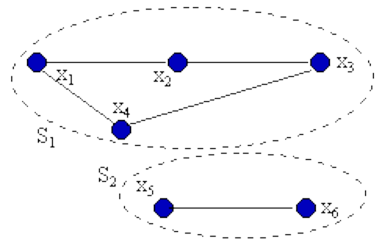
\includegraphics[scale=0.8]{Imagens/intra-grafo.pdf}
\caption{Grafo com representação de Rede de Coautoria intra grupos}
\label{grafo1}
\end{figure}

\begin{figure}[H]
\centering
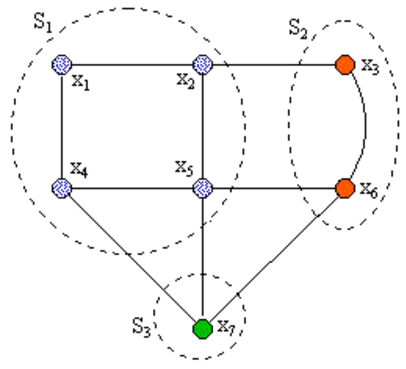
\includegraphics[scale=0.8]{Imagens/inter-grafo.pdf}
\caption{Grafo com representação de Rede de Coautoria inter grupos}
\label{grafo2}
\end{figure}

\section{\textbf{Análise de Redes Sociais}}\label{sec:redes_sociais}

Conforme \citep{Silva2006}, a análise de redes sociais interessa a pesquisadores de vários campos do conhecimento que, na tentativa de compreender o seu impacto sobre a vida social, deram origem a diversas metodologias de análise que têm como base as relações entre os indivíduos, em uma estrutura em forma de redes.

A análise de redes sociais (ARS ou SNA, da expressão em inglês \textit{Social Network Analysis)} é uma abordagem oriunda da sociologia, da psicologia social e da antropologia. \citep{freeman1996some,wasserman1994social}. ARS não é algo recente, há estudos, como o trabalho de \citep{otte2002social} que buscou desde a década de 1970, análises de redes de informação, de pesquisadores e de citações, como também de redes de coautoria.

 Redes de couatoria utiliza-se da análise de redes sociais embasada nas propriedades e aplicações de redes complexas, a qual vemos a seguir.


\begin{figure}[H]
\centering
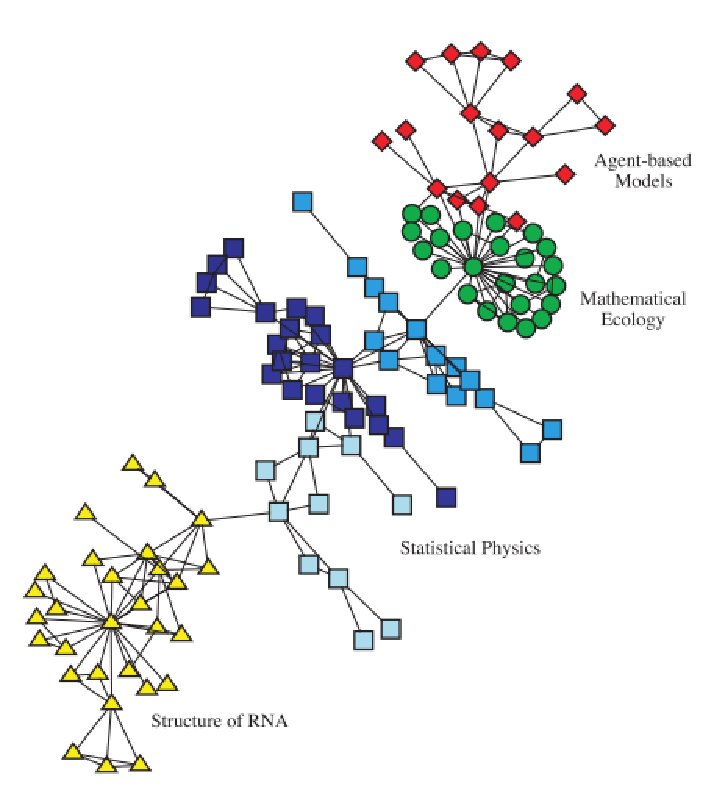
\includegraphics[scale=0.7]{Imagens/rede-newman.pdf}
\caption{Pequena Rede de Coautoria de Newman}
\label{rede1}
\end{figure}

\section{\textbf{Redes Complexas}}\label{sec:redes_complexas}

No contexto da teoria de redes complexas, uma rede corresponde a um grafo, que se representa por um conjunto de nós ligados por arestas, que em conjunto formam uma rede.  Esta rede ou grafo, permite representar relações com fundamento das propriedades dos vários tipos de grafos e como são constituídos, ou seja, como se agrupam os seus nós e são ligadas suas arestas %\cite{mendes2005fisica}.

As propriedades de redes complexas às quais utilizaremos nesse trabalho se encontram definidas a seguir.

\noindent \textbf{Definição 2.3.1} (Grau de um nó). O número de vértices adjacentes a um determinado vértice $x_i$ chama-se de grau de $x_i$. Em um grafo direcionado $\Vec G = (\bm V,\bm \Vec E)$, diferenciamos o grau de saída (output) do grau de entrada (input):

\begin{equation}
k^{out}_{x_{i}}(\Vec{G}) = \sum_{x_j \in V : x_j \neq x_i}^{} A[x_i,x_j]
\label{eq:grauOutput}
\end{equation}

\begin{equation}
k^{in}_{x_{i}}(\Vec{G}) = \sum_{x_j \in V : x_j \neq x_i}^{} A[x_j,x_i]
\label{eq:grauInput}
\end{equation}

Desse modo, chamamos de grau de $x_i$: 

\begin{equation}
k_{x_i}(\Vec{G}) = k^{out}_{x_{i}}(\Vec{G}) + k^{in}_{x_{i}}(\Vec{G})
\label{eq:grau}
\end{equation}

\noindent \textbf{Definição 2.3.2} (Centralidade de um nó - \textit{Degree centrality}). Definida como o número de ligações incidentes de um vértice, esta medida nos informa qual a probabilidade de um vértice receber alguma informação da rede. Logo, a centralidade de um vértice $v$ de um grafo $G = (\bm V,\bm E)$ é dada por:

\begin{equation}
    C_D(\bm v) = deg(\bm v)
\end{equation}

Uma vez que a direção das arestas podem influenciar o cálculo, em redes direcionadas existem duas medidas distintas de centralidade de grau: indegree, que corresponde ao número de ligações direcionadas para o nó e outdegree, que consiste no número de ligações que o nó encaminha para os demais vértices da rede. 

\noindent \textbf{Definição 2.3.3} (Intermediação - \textit{Betweenness centrality}). Trata-se de uma medida de centralidade de um grafo baseada em caminhos mínimos. A intermediação de um nó $v$ é dada do seguinte modo: 

\begin{equation}
    g(\bm v) = \sum_{s \neq t \neq v} \frac{\sigma_{st}(v)}{\sigma_{st}}
\end{equation}

Onde $\sigma_{st}$ é o número total de caminhos mínimos do nó $s$ para o nó $t$ e $\sigma_{st}(v)$ é o número de caminhos mínimos de $s$ para $t$ que utilizam o nó $v$ como intermediário.

 A intermediação também pode ser normalizada, sem perda de precisão, dividindo seu resultado pelo número de pares de nós não incluindo $v$, de maneira que $g(\bm v) \in [0,1]$. Tal medida é vista como mais poderosa que apenas a conectividade, uma vez que fornece uma informação mais global sobre a rede em questão.

\noindent \textbf{Definição 2.3.4} (Proximidade - \textit{Closeness Centrality}). Em um grafo conectado, a proximidade de um nó é uma medida de centralidade calculada pela inversa da soma do comprimento dos caminhos mínimos entre um dado nó $v$ e todos os demais nós do grafo. Desse modo, quanto mais central for o nó, mais próximo dos demais esse se encontrará. Sua fórmula é definida como:

\begin{equation}
    C(\bm v) = \frac{1}{\sum_{\forall u \in V, u\neq v}d_G(u,v)}
\end{equation}

Onde, $d(u,v)$ é a distância do caminho mínimo entre $u$ e $v$.

Usualmente, na literatura costuma-se usar sua versão normalizada, dada não mais pela soma de seus caminhos mínimos e sim pela média destes, como visto a seguir:

\begin{equation}
    C(\bm v) = \frac{N - 1}{\sum_{\forall u \in V, u\neq v}d_G(u,v)}
\end{equation}

Onde, $N$ é o número de nós do grafo, ou seja, $N = |V|$. Para grafos extremamente grandes a diferença $- 1$ torna-se irrelevante, podendo ser descartada.

%\noindent \textbf{Definição 2.3.5} (Diâmetro). É definido como a excentricidade máxima entre dois nós. A excentricidade de um nó $x_i$ é definida como a distância máxima de $x_i$ a todos os outros nós do grafo $G$.

\noindent \textbf{Definição 2.3.5} (Coeficiente de agregação ou aglomeração - \textit{clustering coefficient}). Trata-se do número de ligações entre os vizinhos mais próximos de um nó.

\noindent \textbf{Definição 2.3.6} (Redes estáticas/dinâmicas). Uma rede é estática quando não há variação do número de nós e, é dinâmica, quando é possível modelar o seu crescimento pela análise da variação da sua estrutura ao longo do tempo.

Os estudos das medidas de centralidade de redes foram evoluindo ao longo do tempo; centralidade, proximidade e intermediação é apontada por \citep{freeman1996some}, como medidas essenciais aos estudos e análises de redes. 

A figura abaixo ilustra a topologogia das medidas de centralidade: a) \textit{degree centrality}; b) \textit{closeness centrality} e c) \textit{betweeness centrality}. Com elas podemos perceber por meio dos vértices de cor vermelha a disposição dos mesmos na topologia da rede, e seus respectivos posicionamaentos, nos levando a compreender o tipo da sua centralidade e seu papel na rede.

\begin{figure}[H]
\centering
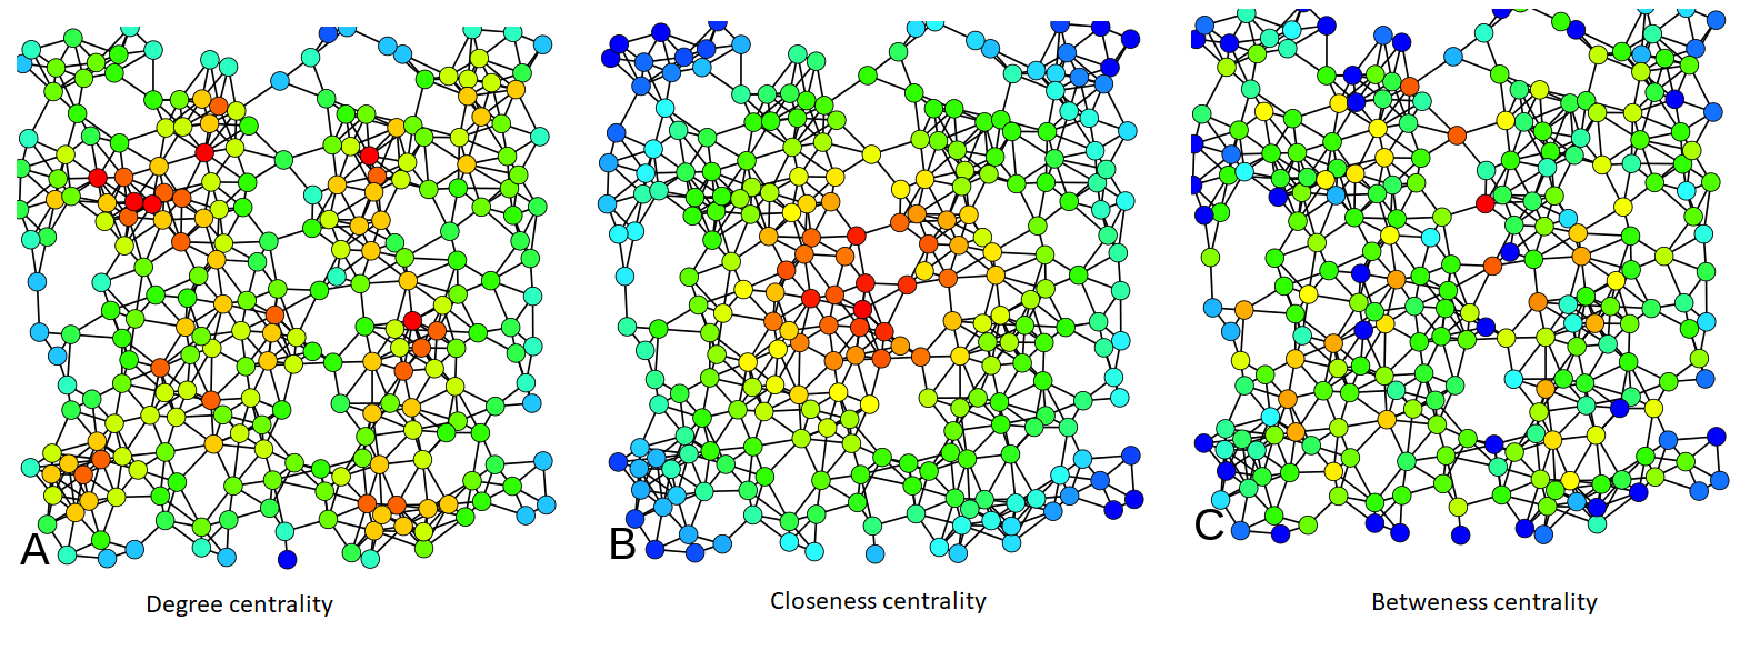
\includegraphics[scale=0.5]{Imagens/Centrality.pdf}
\caption{Redes com ilustração das medidas de centralidade (Fonte: Claudio Rocchini - Adaptado)}
\label{centrality}
\end{figure}

\section{\textbf{Colaboração Científica}}\label{sec:colab} 

Colaboração científica pode ser definida como interação que ocorre dentro de um contexto social entre dois ou mais cientistas, que facilita a partilha de significado e conclusão de tarefas em relação a um objetivo mútuo, compartilhado e organizado. Os cientistas que colaboram também podem trazer metas individuais adicionais para uma colaboração. \citep{Sonnenwald}

Ainda, segundo a autora, a colaboração ocorre dentro do contexto social da ciência, que inclui elementos como a revisão por pares, sistemas de prêmios, paradigmas científicos, políticas de ciência nacionais e internacionais, bem como normas implícitas ao campo disciplinar das instituições de pesquisa e/ou universidades. 

Conforme \citep{Newman2004}, há algum tempo se percebe que a coautoria de artigos em periódicos acadêmicos fornece uma janela sobre padrões de colaboração dentro da comunidade acadêmica. 

Para \citep{Sonnenwald}, estudos da colaboração científica está aumentando, por possuir o potencial de auxiliar a resolução de problemas científicos complexos e promover agendas políticas, econômicas e sociais. 

\resumocap{Neste Capítulo, explanamos os conhecimentos e fundamentações teóricas necessárias para este trabalho. No Capítulo seguinte é apresentada a metodologia utilizada para o desenvolvimento deste.}


\mychapter{\textsc{Metodologia}}{chp:metodologia}
\lhead{\textsc{Metodologia}}

% Breve resumo do capítulo. 
\lettrine{E}{ste} capítulo descreve a metodologia utilizada neste trabalho, descrevendo suas respectivas etapas.

%\section{\textbf{Metodologia}} 

A metodologia utilizada para a presente pesquisa utiliza um modelo exploratório que consiste em quatro etapas cíclicas: 
a)~definição da rede, 
b)~tratamentos de dados da rede; 
c)~determinação das características estruturais e 
d)~inspeção visual \citep{de2018exploratory}.

A definição da rede resultou da coleta dos dados realizada no portal da SciELO\footnote{http://static.scielo.org}. 
Foram  realizados tratamentos desses dados normalizando a padronização os campos da Unidade Federativa (UF). 
A base foi complementada pela informação da localidade geográfica associando os estados (UF) às regiões do Brasil. 
%%% ACF Escreva sempre da forma mais simples e direta possível, a seguinte frase poderia ser "Documentos de origem estrangeira foram definidos como ``Exterior''.
%% Documentos de origem estrangeira foram definidos como ``Exterior''.
%%% VLR Frase reescrita 
%%% VLR documentos do Exterior foram excluídos do escopo

Os dados foram coletados no sítio eletrônico da SciELO a partir do endereço \url{http://static.scielo.org/tabs/tabs_bra}. Os dados associam os documentos publicados em coautoria de um autor com sua respectiva instituição de origem por um ID. O conjunto de dados amostral utilizado para esta pesquisa compreende o período entre 2008 à 2017 e os documentos relacionados as Universidades Federais do país.  

Foi utilizado o ambiente de desenvolvimento \texttt{R-Project} \citep{Rprog}, com uso do \texttt{RStudio} \citep{Rstudio}, possibilitando que o resultado deste trabalho seja coberto ponta a ponta com a mesmo código, facilitando assim a reprodutibilidade desta pesquisa.

O total de documentos indexados coletados da base de dados resultou um montante de 1.302.659 documentos, sendo um total de 112.762 para área de \textit{Health Sciences}, 84.437 para área de \textit{Agricultural Sciences} e 15.278 para \textit{Exact and Earth Sciences}

A produção dos resultados teve por fundamento a teoria dos grafos e na análise de redes sociais, onde buscou a aplicação das métricas de redes complexas, para a compreensão do comportamento das redes de coautoria do presente estudo.

Este trabalho utilizou-se da linguagem \texttt R com o uso dos pacotes \texttt{tidyverse}, \texttt{igraph}, \texttt{ggraph}, \texttt{sna} e \texttt{visNetwork}. A seguir descrevemos as etapas cíclicas proposta por \citep{de2018exploratory} para estudos relacionados ARS.

\section{\textbf{Definição da rede}}

As redes objeto de estudo desta pesquisa é a relação de coautoria existentes nos documentos indexados na base de dados da SciELO, objetivando a criação de um modelo exploratório. Foram definidas as redes de coautoria segregadas pela Unidade Federativa (UF) e Região Geográfica do Brasil para as Universidades Federais do país. Redes de coautoria são classificadas como não-direcionada, ou seja, as ligações existentes entre os vértices independem de uma orientação ou direção.

Os vértices da rede são as Unidades Federativas (UF), agrupadas pelas instituições federais às quais fazem parte da mesma, as arestas as ligações refere-se a ocorrência de coautoria entre as instituições das UF. As arestas são valoradas possuindo pesos pela frequência de ocorrência das coautorias, os vértices são ponderados pelo volume de coautorias, bem como pelos laços, ou seja, as coautorias realizadas entre instituições da mesma UF. %Para este trabalho e por fins topológicos das redes, desconsideramos os pesos para o cálculo das métricas, resultando apenas para inspeção visual das redes geradas.


\section{\textbf{Tratamento de dados da rede}}

Nesta etapa foram elaborados alguns tratamentos da rede, tal como limpeza e padronização de alguns dados, de forma mínima e minuciosa, para evitar que a reprodutibilidade reste prejudicada. Buscamos a padronização dos nomes das Unidades Federativas, e a associação de suas respectivas região geográfica.

As Universidades Federais do Brasil foram agrupadas por estados sendo representadas pelo nome no Estado (UF - Unidade Federativa). Foram realizadas rotinas de geração das matrizes e \textit{datasets} necessários aos cálculos das métricas, tal como a plotagem das redes e gráficos.

\section{\textbf{Determinação das características estruturais}}

Conforme \citet{de2018exploratory} a exploração de uma rede pelas métricas que descrevem sua caracterização estrutural é uma forma mais concisa e precisa quando comparada a inspeção visual, no entanto as métricas por vezes são abstratas e de difícil interpretação. Por isso, deve-se utilizar ambas abordagens analíticas as métricas estruturais da rede e sua observação gráfica.

Foram escolhidas as métricas básicas do número de vértices e arestas, grau médio do vértice, diâmetro da rede, e distância média, centralidade do grau, centralidade de proximidade, e centralidade de intermediação, que foram aplicadas ao período em análise de 2008 à 2017 para a área de \textit{Health Science}. As métricas aferidas denotam de forma quantitativa o comportamento da colaboração científica com bases nas redes de coautoria geradas.

\section{\textbf{Inspeção visual}}

Uma forma enriquecedora de análise de redes sociais é a observação gráfica, para isso são gerados gráficos das redes para representar suas relações e permitir por análise visual a o conhecimento da dinâmica existente pela disposição dos vértices e arestas.

Primeiramente insta ressaltar que no estudos iniciais e exploratórios da base SciELO foram encontradas diversos tipos de instituições de ensino e pesquisa, e que para o objeto do estudo deste trabalho os escopos das redes foram definidos pelas coautorias existentes entre as Universidades Federais do país em suas respectivas Unidades Federativas (UF). 

A análise das redes de coautoria consistiu em uma perspectiva regional explorando suas propriedades e caraterísticas. Foram definidos a área de \textit{Health Sciences} e o período compreendido entre 2008 à 2017, considerando a rede global que consiste todas as Universidades Federais do Brasil agrupadas pelo Estado (UF - Unidade Federativa) a que correspondem. E outra rede tendo como vértice local (ou focal) a Unidade Federativa Alagoas, de maneira a se observar a dinâmica de interação e evolução dessas redes em um prisma analítico e comparativo das redes de coautoria ao longo do tempo.

Os resultados obtidos (gráficos e numéricos) permitem-nos obter um conhecimento descritivo das interações existentes na relação de coautoria entre as relaçõe de coautorias estudas da base SciELO. No aspecto gráfico as arestas possuem espessuras maior ou menor de acordo com o peso definido pelo número de publicações em coautoria, assim, as UF que possuem interações mais fortes ou mais fracas. 

Os vértices foram definidos de um mesmo tom de cor para representar a região geográfica do país a qual pertence a UF, a espessura do laço do vértice detona também o volume de coautorias realizadas dentro da mesma UF.

\resumocap{Neste Capítulo foram apresentadas as quatros etapas da metodologia utilizada: determinação da rede, tratamento de dados, determinação das características estruturais, inspeção visual. No capítulo seguinte apresentamos as análises e interpretações dos resultados.}
\mychapter{\textsc{Resultados e Análises}}{chp:resultados}
\lhead{\textsc{Resultados e Análises}}

%Breve resumo do capítulo.
\lettrine{C}{om} a aplicação dos métodos explanados e a fundamentação teórica referendada, apresentamos os resultados, contextualizando com o problema central deste trabalho e objetivos propostos. 

Para a apresentação dos resultados subdividimos este capítulo em quatro partes, sendo as três primeiras referindo-se a cada uma das áreas pesquisadas, são elas: Características Estruturais das Redes, Medidas de Centralidade, Ranking das Medidas de Centralidade e Discussão dos Resultados.

Na primeira parte apresentamos os resultados das topologias das redes, número de vértices e arestas, características estruturais, densidades, coeficientes de clusterização. É apresentado também as matrizes de coautorias de cada área para todo o período por área.

Na segunda parte, são apresentadas os resultados das medidas de centralidade de cada rede: centralidade do grau (\textit{degree centrality}),  centralidade de proximidade (\textit{closeness centrality}), centralidade de intermediação (\textit{betweeness centrality}), com a apresentação dos gráficos comparativos entre o posicionamento da Universidade Federal de Alagoas (vértice focal), comparado de forma analítica em relação ao comportamento das medidas médias das Universidades Federais do Brasil, seguindo com as interpretações e análises dos resultados.

Na terceira parte, é apresentado o ranking dos índices aferidos por cada Unidade Federativa (UF) em cada área do conhecimento para cada medida de centralidade.

Na quarta parte, realizamos a discussão dos resultados; contextualizando os resultados das medidas de centralidade com a colaboração científica, entendendo o posicionamento do vértice focal (Alagoas) e o desempenho de cada UF em cada área.

\section{\textbf{Redes de Coutorias - Base SciELO}}

Neste ponto apresentamos a análise do comportamento e dos resultados das medidas de centralidade das redes de coautoria de artigos científicos indexados na base SciELO no período compreendido entre 2008 à 2017 para as áreas de: \textit{Health Sciences}, \textit{Agricultural Sciences}, \textit{Exact and Earth Sciences}.


\subsection{\textbf{Características Estruturais}}

Nesta seção trazemos a tona as características estruturais das redes objeto de estudo, sendo elas determinadas: Rede Brasil, compreendendo as Universidades Federais relacionadas ao respectivo Estado (UF - Unidade Federativa) às quais estão sediadas; para cada área do conhecimento visto acima.

Neste tópico apresentamos a estrutura da Rede Brasil com a finalidade de compreendermos a dimensão e topologia de cada área analisada dentro do período estudado. Na figura \ref{nos-arestas-todos}, verificamos o número de vértices e arestas para cada ano/área.


\begin{table}[H]
	\centering
	\begin{tabular}{lllllll}
		\hline
		\multicolumn{7}{|c|}{\textbf{Topologia: Vértices e Arestas por Área}}                                                                                                                                                                                                                                                                                                                                                                                            \\ \hline
		\rowcolor[HTML]{EFEFEF} 
		\multicolumn{1}{|l|}{\cellcolor[HTML]{EFEFEF}\textbf{Área}} & \multicolumn{2}{c|}{\cellcolor[HTML]{EFEFEF}\textbf{\begin{tabular}[c]{@{}c@{}}Health \\ Sciences\end{tabular}}}               & \multicolumn{2}{c|}{\cellcolor[HTML]{EFEFEF}\textbf{\begin{tabular}[c]{@{}c@{}}Agricultural \\ Sciences\end{tabular}}}         & \multicolumn{2}{c|}{\cellcolor[HTML]{EFEFEF}\textbf{\begin{tabular}[c]{@{}c@{}}Exact and Earth \\ Sciences\end{tabular}}}      \\ \hline
		\rowcolor[HTML]{C0C0C0} 
		\multicolumn{1}{|l|}{\cellcolor[HTML]{C0C0C0}\textbf{Ano}}  & \multicolumn{1}{l|}{\cellcolor[HTML]{C0C0C0}\textbf{Vértices}} & \multicolumn{1}{l|}{\cellcolor[HTML]{C0C0C0}\textbf{Arestas}} & \multicolumn{1}{l|}{\cellcolor[HTML]{C0C0C0}\textbf{Vértices}} & \multicolumn{1}{l|}{\cellcolor[HTML]{C0C0C0}\textbf{Arestas}} & \multicolumn{1}{l|}{\cellcolor[HTML]{C0C0C0}\textbf{Vértices}} & \multicolumn{1}{l|}{\cellcolor[HTML]{C0C0C0}\textbf{Arestas}} \\ \hline
		\multicolumn{1}{|l|}{2008}                                  & \multicolumn{1}{l|}{27}                                        & \multicolumn{1}{l|}{109}                                      & \multicolumn{1}{l|}{25}                                        & \multicolumn{1}{l|}{90}                                       & \multicolumn{1}{l|}{21}                                        & \multicolumn{1}{l|}{63}                                       \\ \hline
		\multicolumn{1}{|l|}{2009}                                  & \multicolumn{1}{l|}{25}                                        & \multicolumn{1}{l|}{122}                                      & \multicolumn{1}{l|}{26}                                        & \multicolumn{1}{l|}{100}                                      & \multicolumn{1}{l|}{25}                                        & \multicolumn{1}{l|}{87}                                       \\ \hline
		\multicolumn{1}{|l|}{2010}                                  & \multicolumn{1}{l|}{25}                                        & \multicolumn{1}{l|}{163}                                      & \multicolumn{1}{l|}{25}                                        & \multicolumn{1}{l|}{154}                                      & \multicolumn{1}{l|}{22}                                        & \multicolumn{1}{l|}{91}                                       \\ \hline
		\multicolumn{1}{|l|}{2011}                                  & \multicolumn{1}{l|}{25}                                        & \multicolumn{1}{l|}{165}                                      & \multicolumn{1}{l|}{27}                                        & \multicolumn{1}{l|}{150}                                      & \multicolumn{1}{l|}{23}                                        & \multicolumn{1}{l|}{88}                                       \\ \hline
		\multicolumn{1}{|l|}{2012}                                  & \multicolumn{1}{l|}{26}                                        & \multicolumn{1}{l|}{181}                                      & \multicolumn{1}{l|}{26}                                        & \multicolumn{1}{l|}{180}                                      & \multicolumn{1}{l|}{24}                                        & \multicolumn{1}{l|}{88}                                       \\ \hline
		\multicolumn{1}{|l|}{2013}                                  & \multicolumn{1}{l|}{26}                                        & \multicolumn{1}{l|}{183}                                      & \multicolumn{1}{l|}{26}                                        & \multicolumn{1}{l|}{178}                                      & \multicolumn{1}{l|}{22}                                        & \multicolumn{1}{l|}{86}                                       \\ \hline
		\multicolumn{1}{|l|}{2014}                                  & \multicolumn{1}{l|}{26}                                        & \multicolumn{1}{l|}{197}                                      & \multicolumn{1}{l|}{27}                                        & \multicolumn{1}{l|}{179}                                      & \multicolumn{1}{l|}{25}                                        & \multicolumn{1}{l|}{83}                                       \\ \hline
		\multicolumn{1}{|l|}{2015}                                  & \multicolumn{1}{l|}{27}                                        & \multicolumn{1}{l|}{194}                                      & \multicolumn{1}{l|}{26}                                        & \multicolumn{1}{l|}{173}                                      & \multicolumn{1}{l|}{22}                                        & \multicolumn{1}{l|}{77}                                       \\ \hline
		\multicolumn{1}{|l|}{2016}                                  & \multicolumn{1}{l|}{26}                                        & \multicolumn{1}{l|}{298}                                      & \multicolumn{1}{l|}{26}                                        & \multicolumn{1}{l|}{182}                                      & \multicolumn{1}{l|}{25}                                        & \multicolumn{1}{l|}{99}                                       \\ \hline
		\multicolumn{1}{|l|}{2017}                                  & \multicolumn{1}{l|}{26}                                        & \multicolumn{1}{l|}{199}                                      & \multicolumn{1}{l|}{25}                                        & \multicolumn{1}{l|}{190}                                      & \multicolumn{1}{l|}{24}                                        & \multicolumn{1}{l|}{94}                                       \\ \hline
	\end{tabular}
\label{nos-arestas-todos}
\caption{Topologia das Redes (Vértices e Arestas) por Ano}
\end{table}


Pela topologia verificamos que as área de \textit{Health Sciences} e \textit{Agricultural Sciences} possuem um maior número de arestas ao logo do tempo quando comparada a \textit{Exact and Earth Sciences}. Destaque para o ano de 2016 em que observamos um pico que eleva o número de arestas no ano de 2016, como visto na tabela \ref{nos-arestas-todos} o que possivelmente neste ano maior número de publicações/indexações foram realizadas, o que resultou o aumento da conectividade da rede, que impactou em sua densidade e também no resultados das medidas de centralidade como veremos a frente. 

Em \textit{Agricultural Sciences} podemos considerar uma normalidade, considerando o número médio de vértices e uma tendência crescente de arestas (coautorias) ao longo do tempo; \textit{Exact and Earth Sciences} possui uma observação curiosa pela oscilação do número de vértices de cada ano, ou seja a desconexão e reconexão destes, mostrando que ao longo do tempo as participações do estados nas coautorias, em outros anos alguns estados deixaram de colaborar e participar da rede.

A tabela \ref{estruturais} abaixo apresenta a densidade e aglomeração (clustering coefficient) para complementar a compreensão da estrutura e dimensão de cada rede, que caracteriza as relações de coautorias existentes em cada área.

\begin{table}[H]
	\centering
	\begin{tabular}{|l|l|l|l|l|l|l|}
		\hline
		\multicolumn{7}{|c|}{\textbf{Características Estruturais da Rede Brasil por Área}}                                                                                                                                                                                                                                                                                                                                 \\ \hline
		\rowcolor[HTML]{C0C0C0} 
		\multicolumn{4}{|c|}{\cellcolor[HTML]{C0C0C0}\textbf{Densidade}}                                                                                                                                           & \multicolumn{3}{c|}{\cellcolor[HTML]{C0C0C0}\textbf{Aglomeração (Clustering Coefficient)}}                                                                                                          \\ \hline
		\rowcolor[HTML]{EFEFEF} 
		Ano  & \begin{tabular}[c]{@{}l@{}}Health \\ Sciences\end{tabular} & \begin{tabular}[c]{@{}l@{}}Agricultural \\ Sciences\end{tabular} & \begin{tabular}[c]{@{}l@{}}Exact and Earth \\ Sciences\end{tabular} & \begin{tabular}[c]{@{}l@{}}Health \\ Sciences\end{tabular} & \begin{tabular}[c]{@{}l@{}}Agricultural \\ Sciences\end{tabular} & \begin{tabular}[c]{@{}l@{}}Exact and Earth \\ Sciences\end{tabular} \\ \hline
		2008 & 0,121                                                      & 0,155                                                            & 0,150                                                                & 0,523                                                      & 0,364                                                            & 0,355                                                               \\ \hline
		2009 & 0,165                                                      & 0,152                                                            & 0,145                                                               & 0,625                                                      & 0,415                                                            & 0,398                                                               \\ \hline
		2010 & 0,230                                                       & 0,258                                                            & 0,197                                                               & 0,726                                                      & 0,557                                                            & 0,506                                                               \\ \hline
		2011 & 0,235                                                      & 0,214                                                            & 0,174                                                               & 0,744                                                      & 0,543                                                            & 0,356                                                               \\ \hline
		2012 & 0,238                                                      & 0,271                                                            & 0,159                                                               & 0,773                                                      & 0,601                                                            & 0,391                                                               \\ \hline
		2013 & 0,242                                                      & 0,271                                                            & 0,186                                                               & 0,772                                                      & 0,619                                                            & 0,429                                                               \\ \hline
		2014 & 0,265                                                      & 0,252                                                            & 0,138                                                               & 0,745                                                      & 0,619                                                            & 0,395                                                               \\ \hline
		2015 & 0,238                                                      & 0,258                                                            & 0,167                                                               & 0,803                                                      & 0,608                                                            & 0,339                                                               \\ \hline
		2016 & 0,418                                                      & 0,282                                                            & 0,165                                                               & 0,943                                                      & 0,642                                                            & 0,489                                                               \\ \hline
		2017 & 0,266                                                      & 0,313                                                            & 0,170                                                                & 0,798                                                      & 0,682                                                            & 0,422                                                               \\ \hline
	\end{tabular}
\caption{Características Estruturais Rede Brasil (2008-2017)}
\label{estruturais}
\end{table}


\subsubsection{\textbf{Matrizes de Coautorias por Unidades Federativas}}

A seguir apresentamos as matrizes de coautorias por Unidades Federativas por área, compreendendo todo o período (2008 à 2017). As matrizes é uma das formas primárias de observar a colaboração científica existente entre os estados, e nos referenciaremos a elas, ao longo das análises dos resultados das medidas de centralidade.

\subsubsection{Health Sciences}

\begin{figure}[H]
	\begin{adjustwidth}{-.6in}{-.6in}
		\centering
		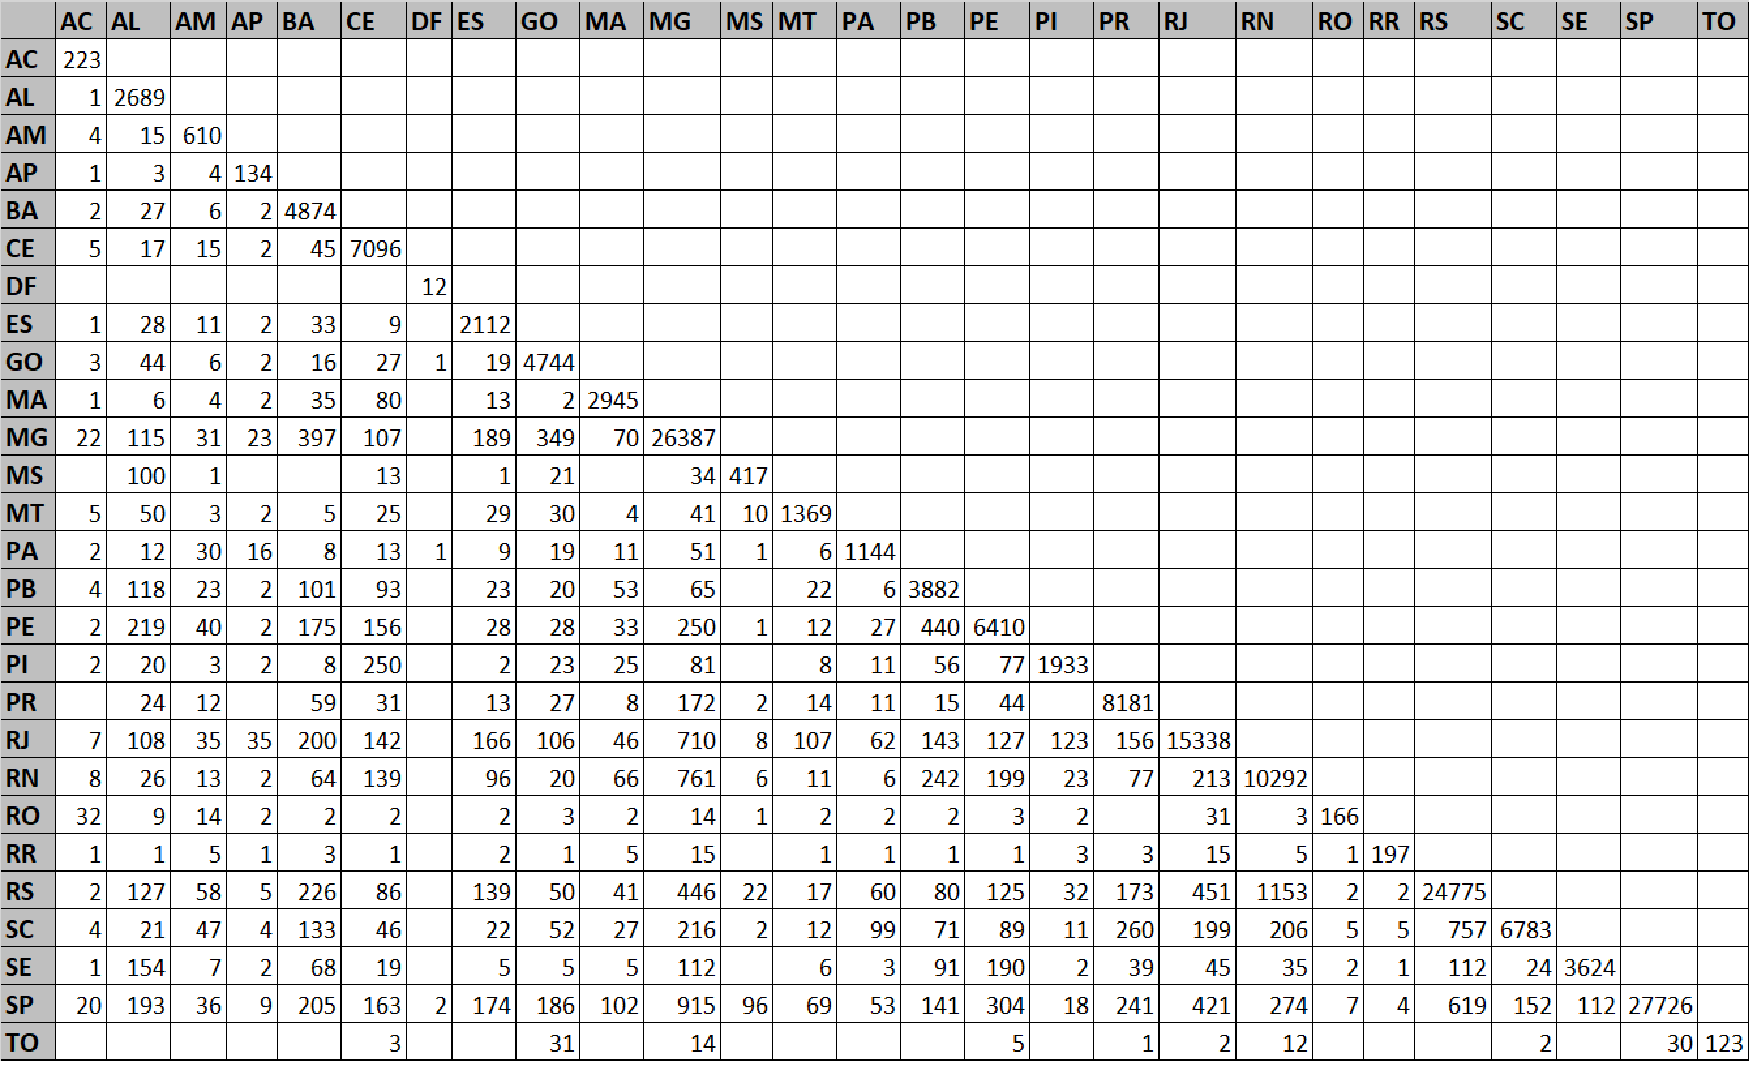
\includegraphics[scale=0.6]{Imagens/health/matriz-uf.pdf}
		\caption{Matriz de Coautorias \textit{Health Sciences} (2008-2017)}
		\label{matriz-uf-agri}
	\end{adjustwidth}
\end{figure}

Observamos para todo período analisado que a matriz na área de \textit{Health Sciences}, os valores absolutos de coautorias entre os estado, denota uma forte conectividade desta rede, quando comparada as áreas de \textit{Agricultural Sciences e Exact and Earth Sciences}, exceto para alguns estados, da região Norte do país, como Tocantins e Roraima. Podemos perceber o grande volume de coautorias existente dentro do mesmo estado, como São Paulo, Rio Grande do Sul, Minas Gerais e Rio de Janeiro.

\subsubsection{Agricultural Sciences}

\begin{figure}[H]
	\begin{adjustwidth}{-.6in}{-.6in}
		\centering
		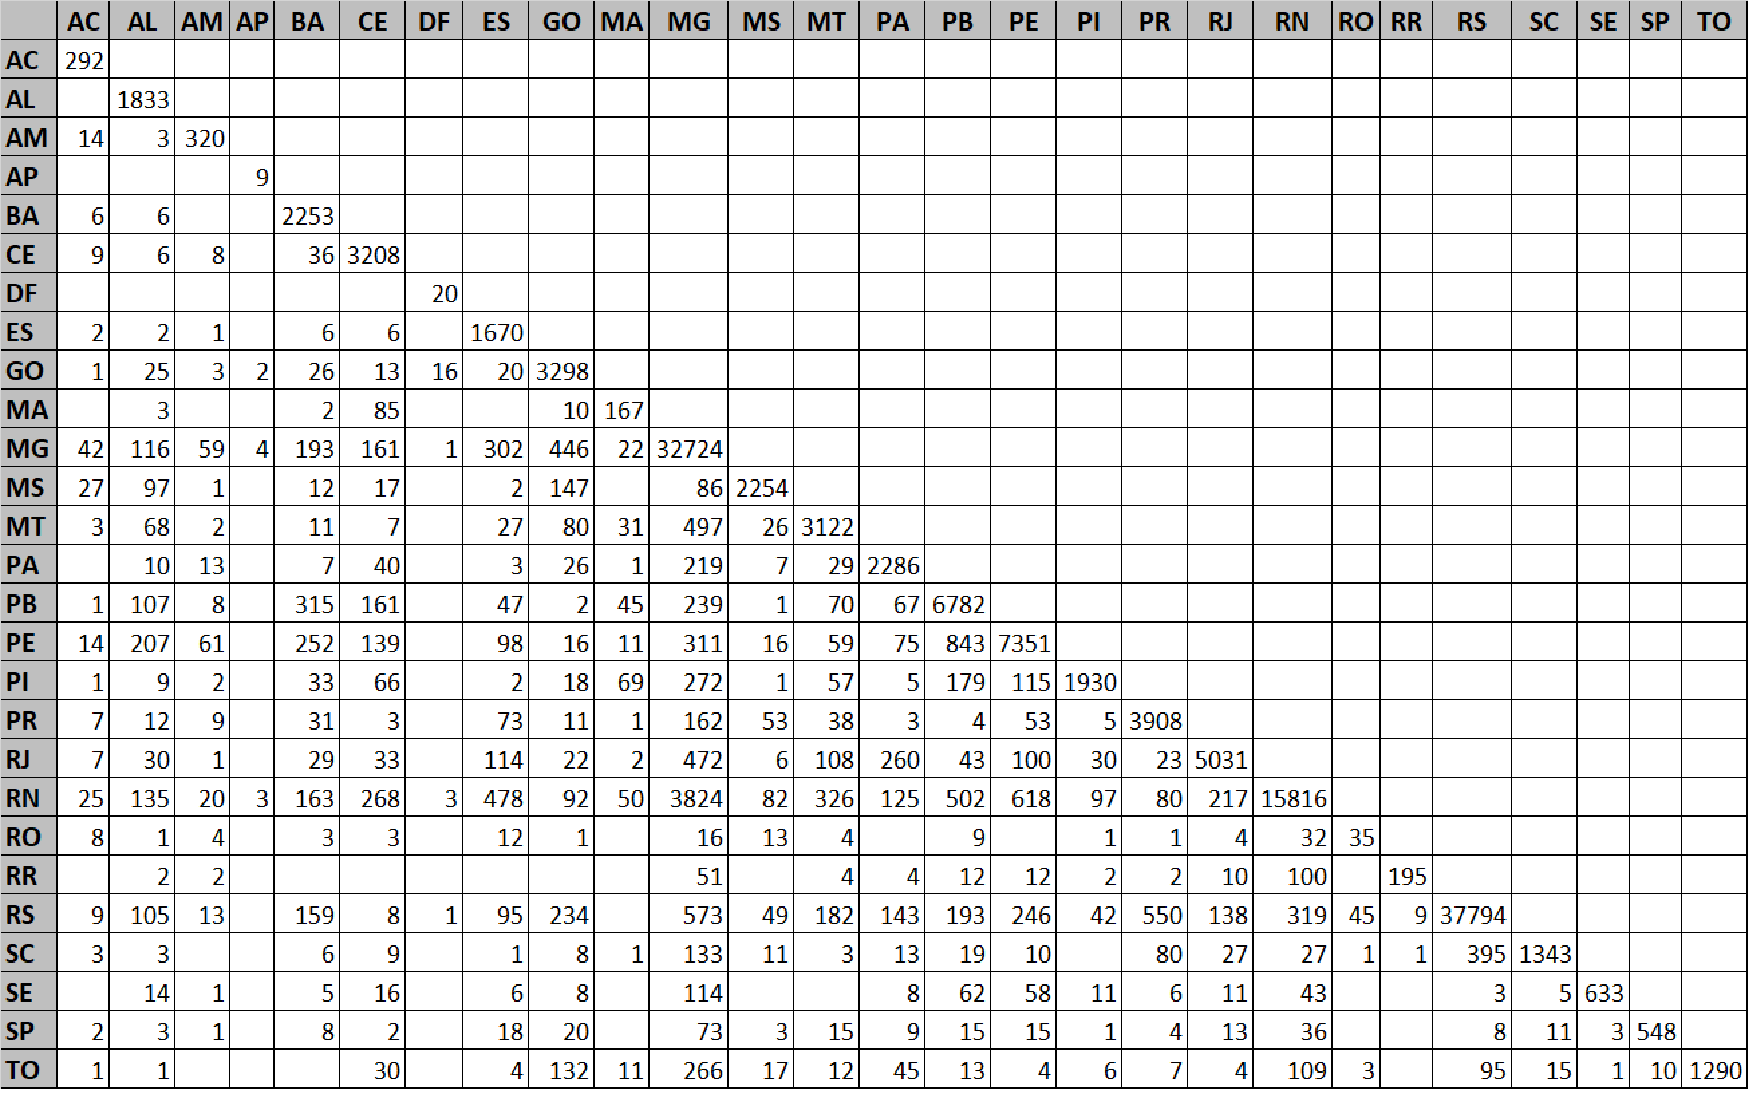
\includegraphics[scale=0.6]{Imagens/agricultural/matriz-uf.pdf}
		\caption{Matriz de Coautorias \textit{Agricultural Sciences} (2008-2017)}
		\label{matriz-uf-agri}
	\end{adjustwidth}
\end{figure}

Com a matriz de coautorias na área de \textit{Agricultural Sciences}, percebemos uma densidade menor e muitas lacunas da colaboração entre alguns unidades federativas, como o Distrito Federal, Roraima, e pouca volume em número de coautorias entre diversos estados. Destaque para o estado do Rio Grande do Sul, e no nordeste o Rio Grande do Norte, que por meio de suas  Universidade Federal do Rio Grande do Norte e da Universidade Federal Rural do Semi-Árido, apresentaram grande participação nas coautorias em Ciências Agrárias.

\subsubsection{Exact and Earth Sciences}

\begin{figure}[H]
	\begin{adjustwidth}{-.6in}{-.6in}
		\centering
		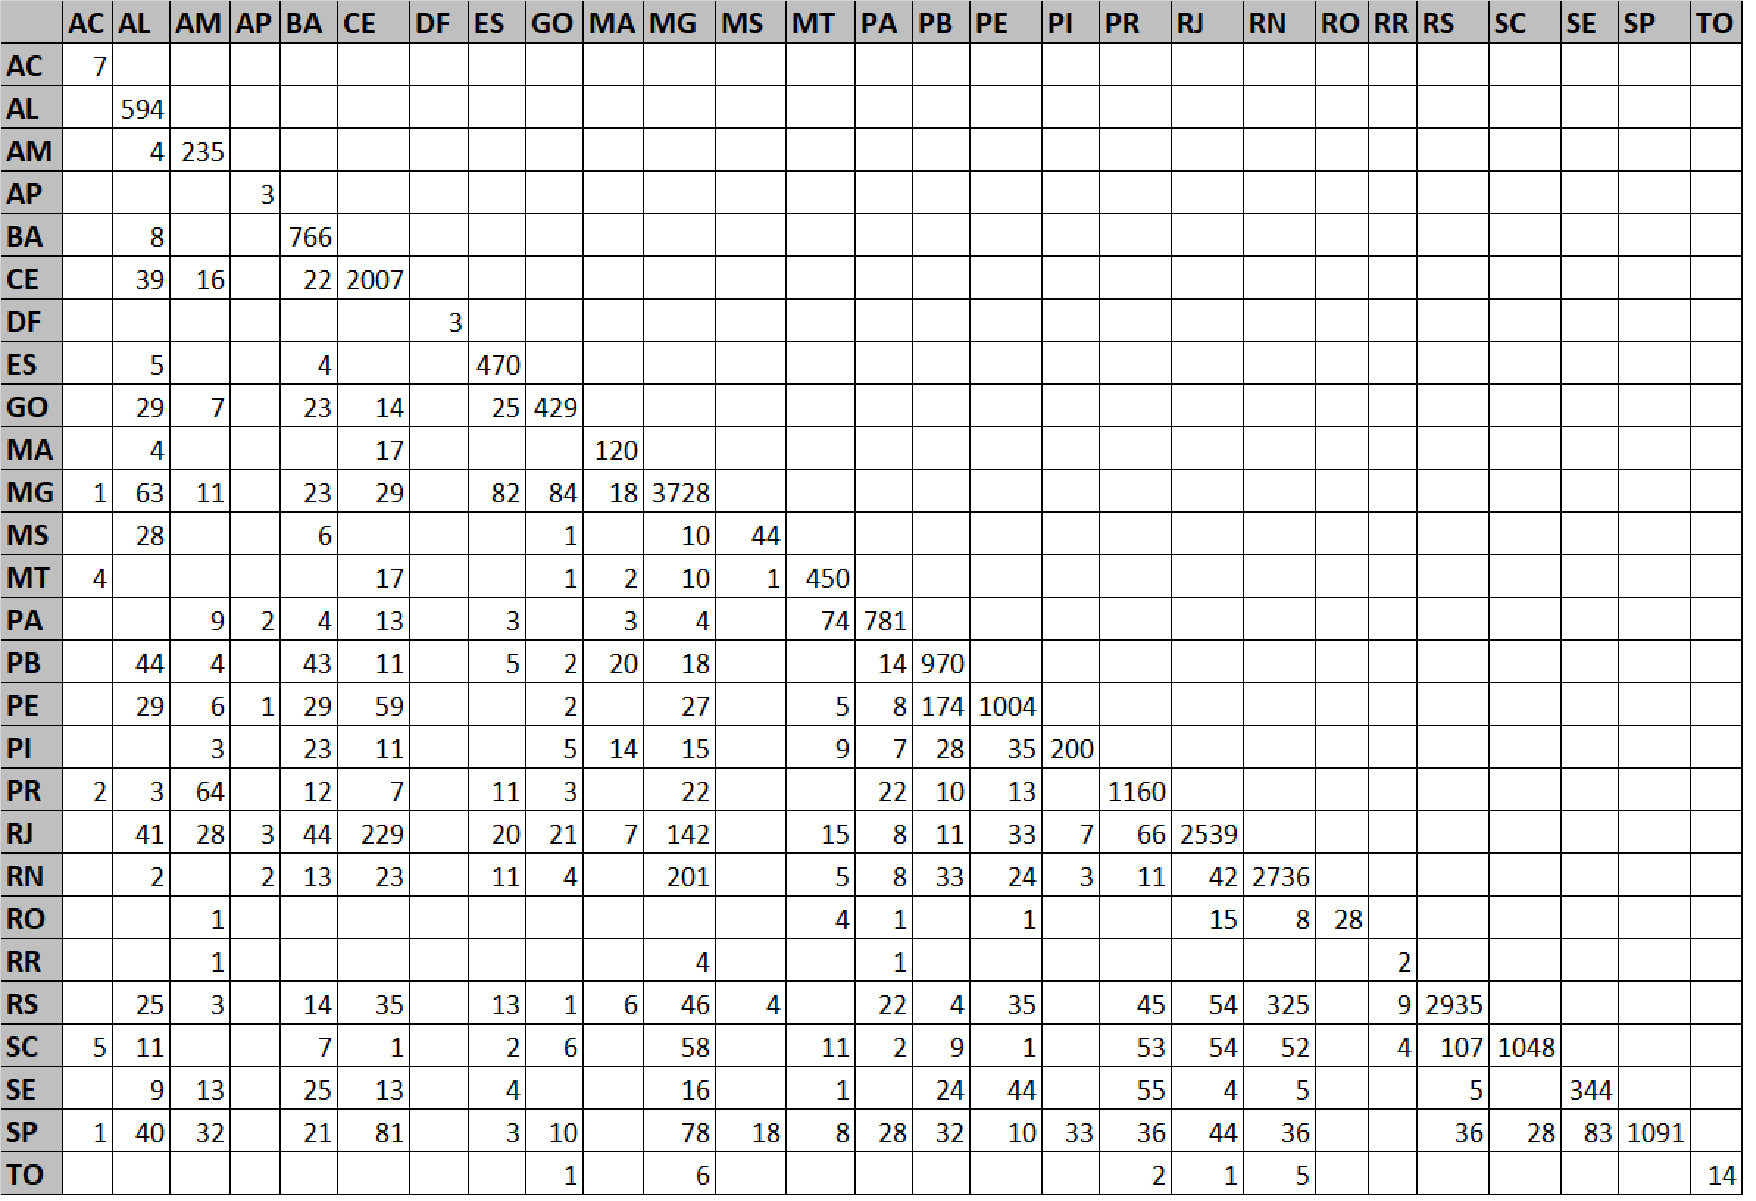
\includegraphics[scale=0.6]{Imagens/exact/matriz-uf.pdf}
		\caption{Matriz de Coautorias \textit{Exact and Earth Sciences} (2008-2017)}
		\label{matriz-agri}
	\end{adjustwidth}
\end{figure}

Em \textit{Exact and Earth Sciences} percebemos que pelo volume de coautoria, a Base SciELO não é um referência para a indexação de artigos nesta área, sua matriz apresenta poucas coautorias, realizada entre alguns estados, apresentando muitas lacunas principalmente em estados do Centro-Oeste e Norte do país. Destaque para Minas Gerais e Rio de Janeiro.

\subsubsection{Visualização da rede}

Para inspeção visual que coaduna com as análises numéricas, postamos a seguir, por seleção aleatória o ano de 2015 a rede de \textit{Agricultural Sciences} para Rede Brasil e Rede Alagoas, trata-se de uma plotagem exemplo uma vez que estamos trabalhando com 60 redes ao total, todas as redes (de cada ano e área) estão disponíveis no Apêndice \ref{redes}.


\begin{figure}[H]
\centering
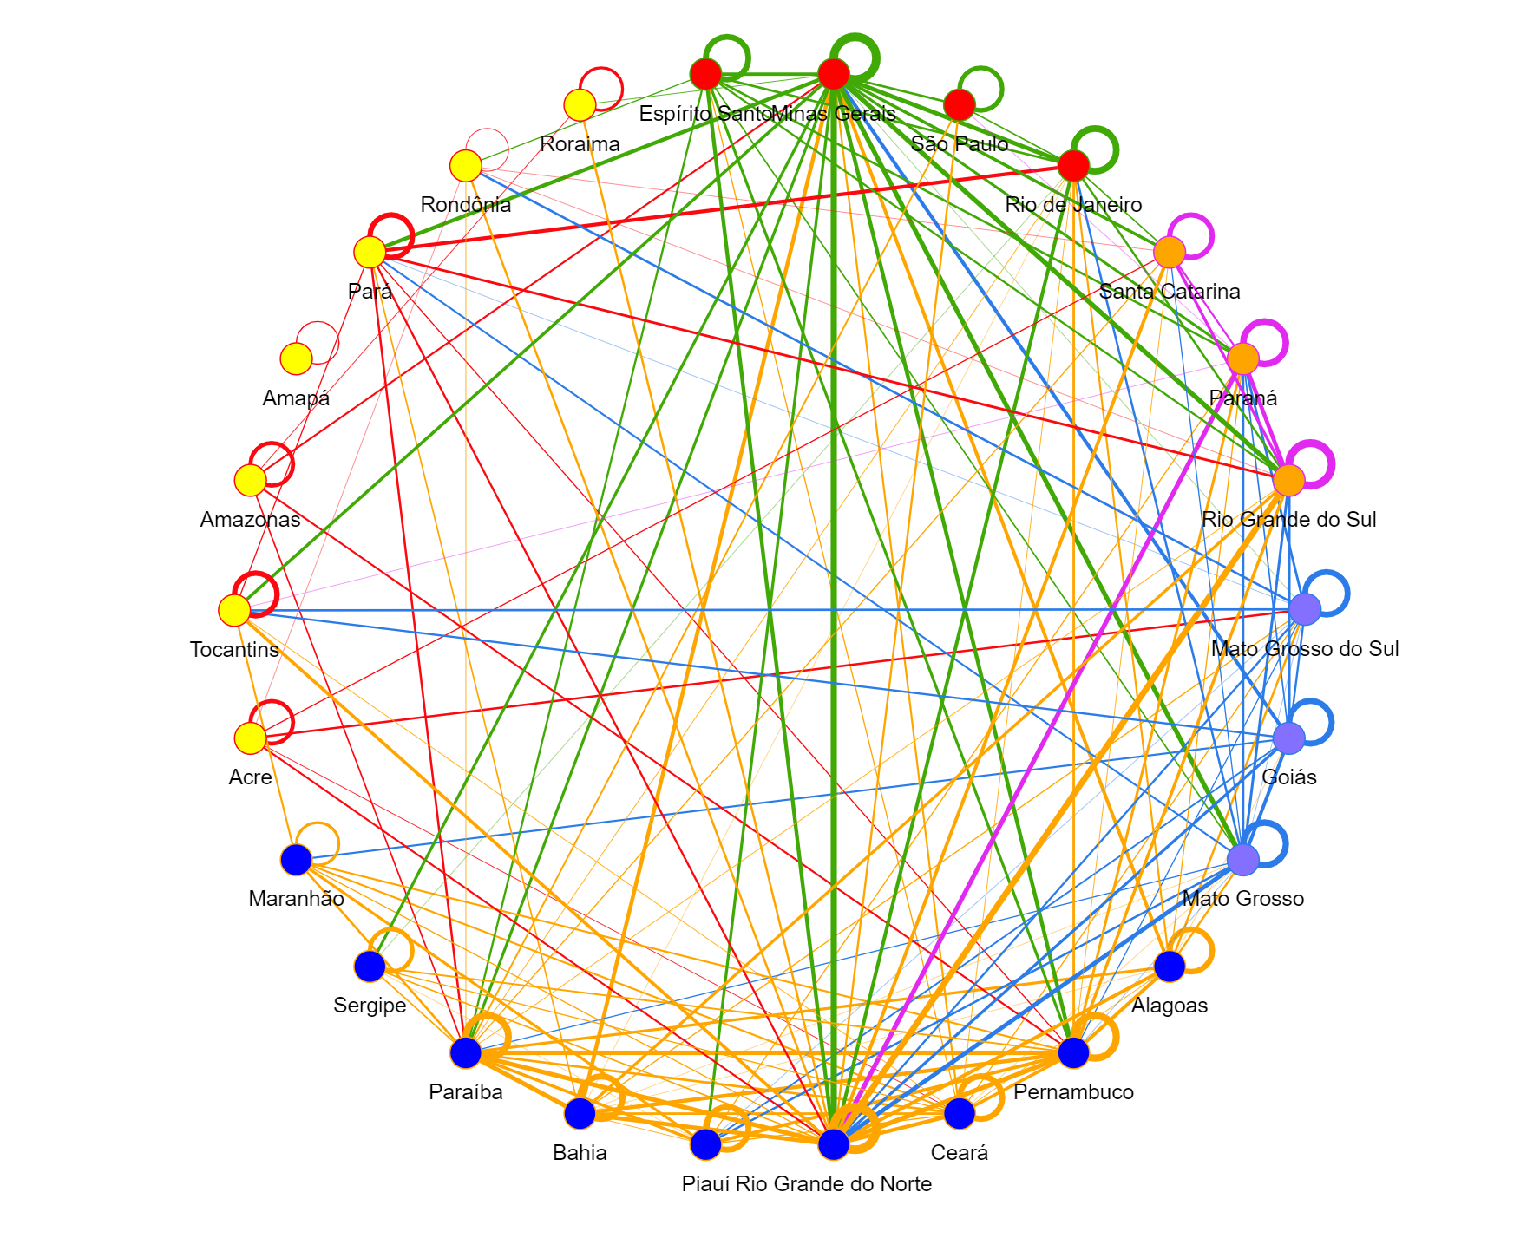
\includegraphics[scale=0.6]{Imagens/rede-agr-br-2015.pdf}
\caption{Rede de Coautoria das Universidades Federais do Brasil - 2015 (\textit{Agricultural Sciences})}
\label{rede-2015-br}
\end{figure}

As características propostas na plotagem da rede é, formato em círculo para fins comparativos, disposição dos vértices com coloração das UF pertencentes a mesma região geográfica, espessura e coloração das arestas indicando o maior volume/peso das coautorias existente entre as UFs, espessuras dos laços, indicando peso das coautorias existentes na mesma UF.

A figura \ref{rede-2015-br} apresenta a rede de coautoria das Universidades Federais do Brasil, composta pelos vértices que representam os Estados (Unidades Federativas - UF) do Brasil e suas ligações (arestas) representando as coautorias existentes entre eles. A figura \ref{rede-2015-al} representa para o mesmo ano e área a rede plotada a partir do vértice Alagoas.

\begin{figure}[H]
	\centering
	\includegraphics[scale=0.6]{Imagens/rede-agr-al-2015.pdf}
	\caption{Rede de Coautoria Vértice Focal Universidade Federal de Alagoas - 2015 (\textit{Agricultural Sciences})}
	\label{rede-2015-al}
\end{figure}

\section{\textbf{Medidas de Centralidade}}

Nesta seção, após a análise das características estruturais das Redes Brasil para cada área do conhecimento, determinamos o vértice focal de Alagoas, como Rede Alagoas, representado pela Universidade Federal de Alagoas, como ponto de interesse para uma avaliação do posicionamento e desempenho desta rede/vértice em comparação a Rede Brasil (média). Sendo esta, organizada por subseções para cada medida de centralidade.

Após a análise de cada medida, será apresentado um Ranking por cada área do e o o respectivo índice médio do período (2008-2017) para cada Unidade Federativa (UF). 

Válido ressaltar que foge ao escopo desse trabalho o entendimento de fatores exógenos ou específicos que não seja o do estudo das medidas de centralidade aplicadas a avaliação da colaboração científica, considerando que há várias possibilidades de investigações \textit{drill-down} que possam detalhar conhecimento complementares a respeito das coautorias. Os gráficos estão plotados em resolução maior no Apêndice \ref{graficos}.

\subsection{\textbf{Centralidade do Grau}}

Esta medida indica o melhor posicionamento dos vértices utilizando o parâmetro que possuem o maior número de ligações entre outros vértices, ou seja, a partir desse ponto de vista são vértices mais influentes, observaremos graficamente como se comportou a Rede Alagoas face a média da Rede Brasil.

A tabela \ref{degree-tab} apresenta os resultados da centralidade do grau para todas áreas comparando a Rede Brasil (média) e Alagoas.

\begin{table}[H]
	\centering
	\begin{tabular}{|l|l|l|l|l|l|l|}
		\hline
		\multicolumn{7}{|c|}{\textbf{\begin{tabular}[c]{@{}c@{}}Centralidade do Grau  \\ (Degree centrality) por Área\end{tabular}}}                                                                                                                                                                                                                                                          \\ \hline
		\rowcolor[HTML]{C0C0C0} 
		\textbf{Ano}  & \multicolumn{2}{c|}{\cellcolor[HTML]{C0C0C0}\textbf{\begin{tabular}[c]{@{}c@{}}Health \\ Sciences\end{tabular}}} & \multicolumn{2}{c|}{\cellcolor[HTML]{C0C0C0}\textbf{\begin{tabular}[c]{@{}c@{}}Agricultural \\ Sciences\end{tabular}}} & \multicolumn{2}{|c|}{\cellcolor[HTML]{C0C0C0}\textbf{\begin{tabular}[c]{@{}c@{}}Exact and \\ Earth Sciences\end{tabular}}} \\ \hline
		\rowcolor[HTML]{EFEFEF} 
		\textbf{Rede} & \textbf{Brasil}                                        & \textbf{Alagoas}                                        & \textbf{Brasil}                                           & \textbf{Alagoas}                                           & \textbf{Brasil}                                             & \textbf{Alagoas}                                            \\ \hline
		2008          & 6,29                                                   & 7                                                       & 7,44                                                      & 5                                                          & 8,19                                                        & 2                                                           \\ \hline
		2009          & 7,92                                                   & 7                                                       & 7,62                                                      & 8                                                         & 10,24                                                       & 14                                                          \\ \hline
		2010          & 11,04                                                  & 15                                                      & 12,40                                                     & 12                                                         & 12,55                                                       & 14                                                          \\ \hline
		2011          & 11,28                                                  & 10                                                      & 11,11                                                     & 13                                                         & 11,30                                                       & 12                                                          \\ \hline
		2012          & 11,92                                                  & 12                                                      & 13,54                                                     & 15                                                         & 10,67                                                       & 18                                                          \\ \hline
		2013          & 12,07                                                  & 14                                                      & 13,54                                                     & 14                                                         & 12,00                                                       & 12                                                          \\ \hline
		2014          & 13,23                                                  & 18                                                      & 13,11                                                     & 13                                                         & 9,44                                                        & 14                                                          \\ \hline
		2015          & 12,37                                                  & 19                                                      & 12,92                                                     & 13                                                         & 10,36                                                       & 6                                                           \\ \hline
		2016          & 20,92                                                  & 24                                                      & 14,08                                                     & 12                                                         & 12,32                                                       & 12                                                          \\ \hline
		2017          & 13,30                                                  & 19                                                      & 15,04                                                     & 15                                                         & 12,17                                                       & 14                                                          \\ \hline
	\end{tabular}
	\caption{Medidas de Centralidade do Grau por Área (2008-2017)}
	\label{degree-tab}
\end{table}

\subsubsection{Health Sciences}

\begin{figure}[H]
\centering
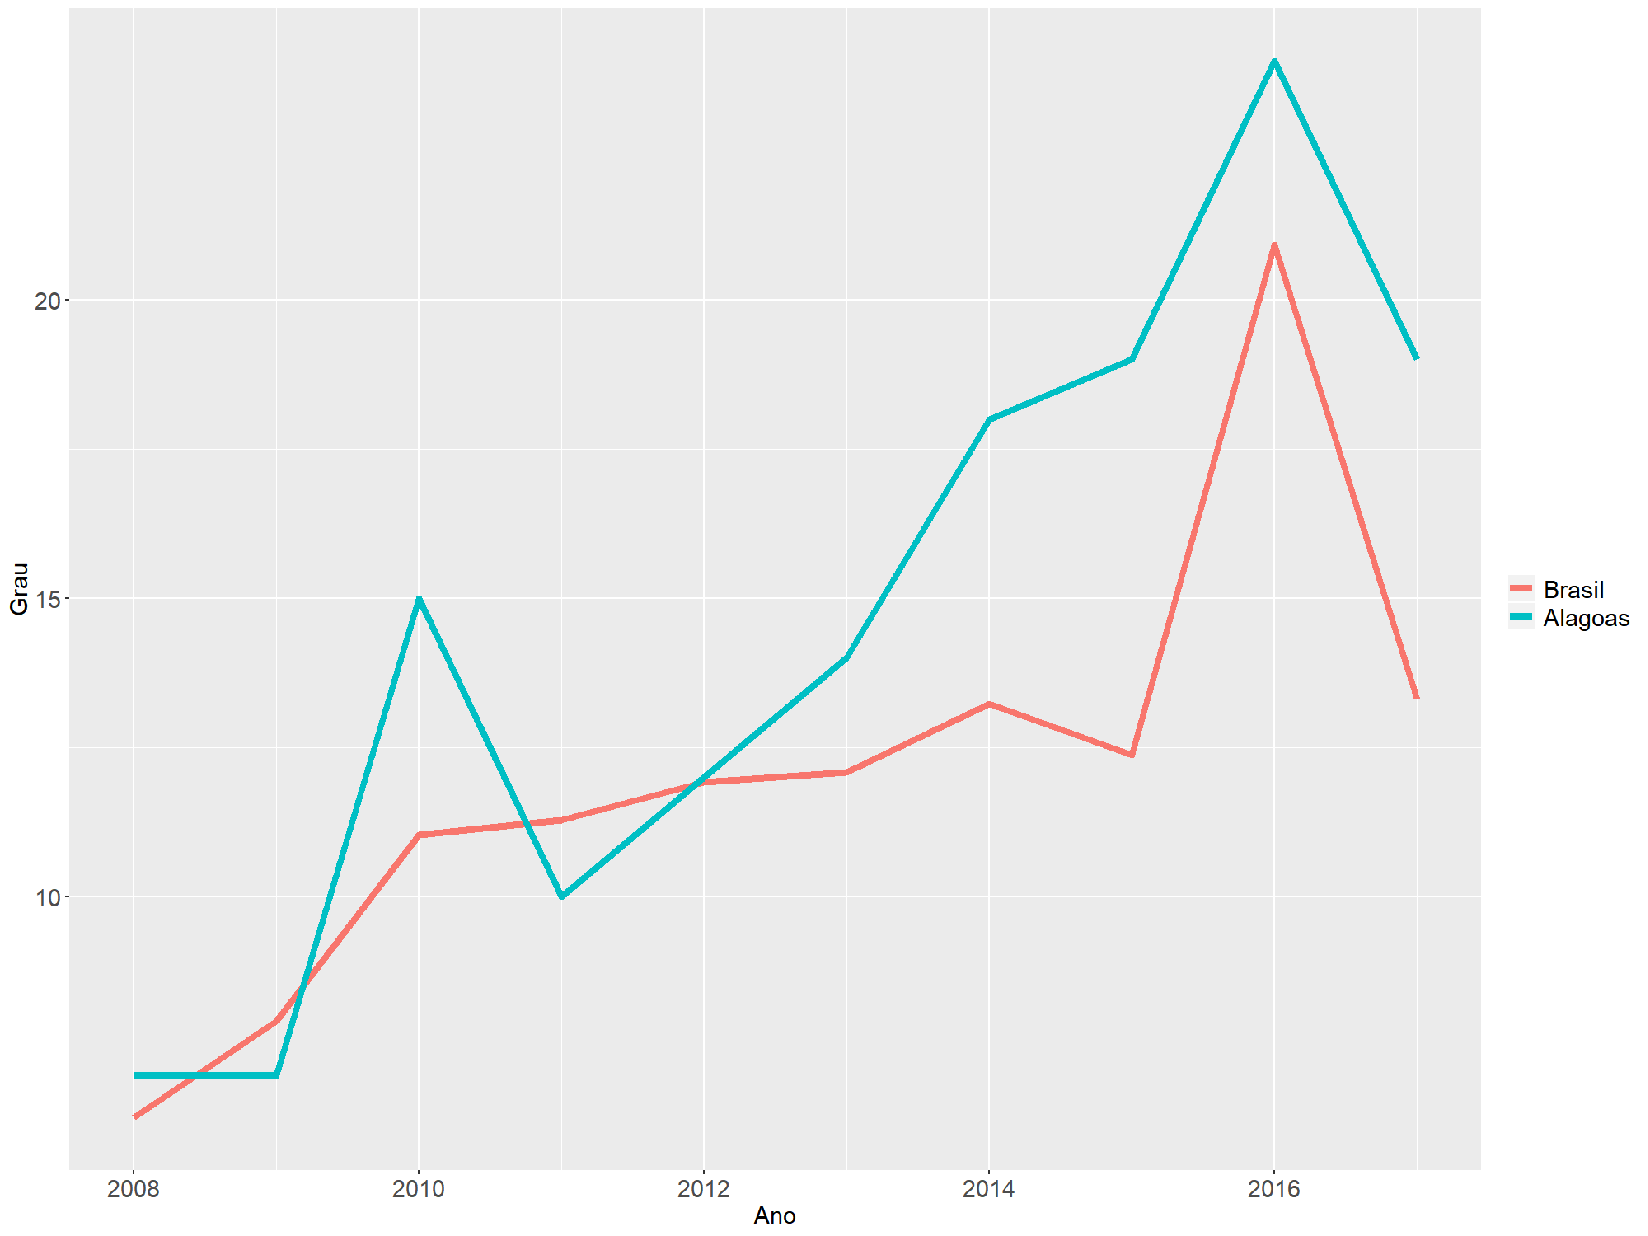
\includegraphics[scale=0.4]{Imagens/graf-linha-degree-br-al.pdf}
\caption{Centralidade do Grau (\textit{Health Sciences})}
\label{degree-health-1}
\end{figure}

\subsubsection{Agricultural Sciences}

\begin{figure}[H]
	\centering
	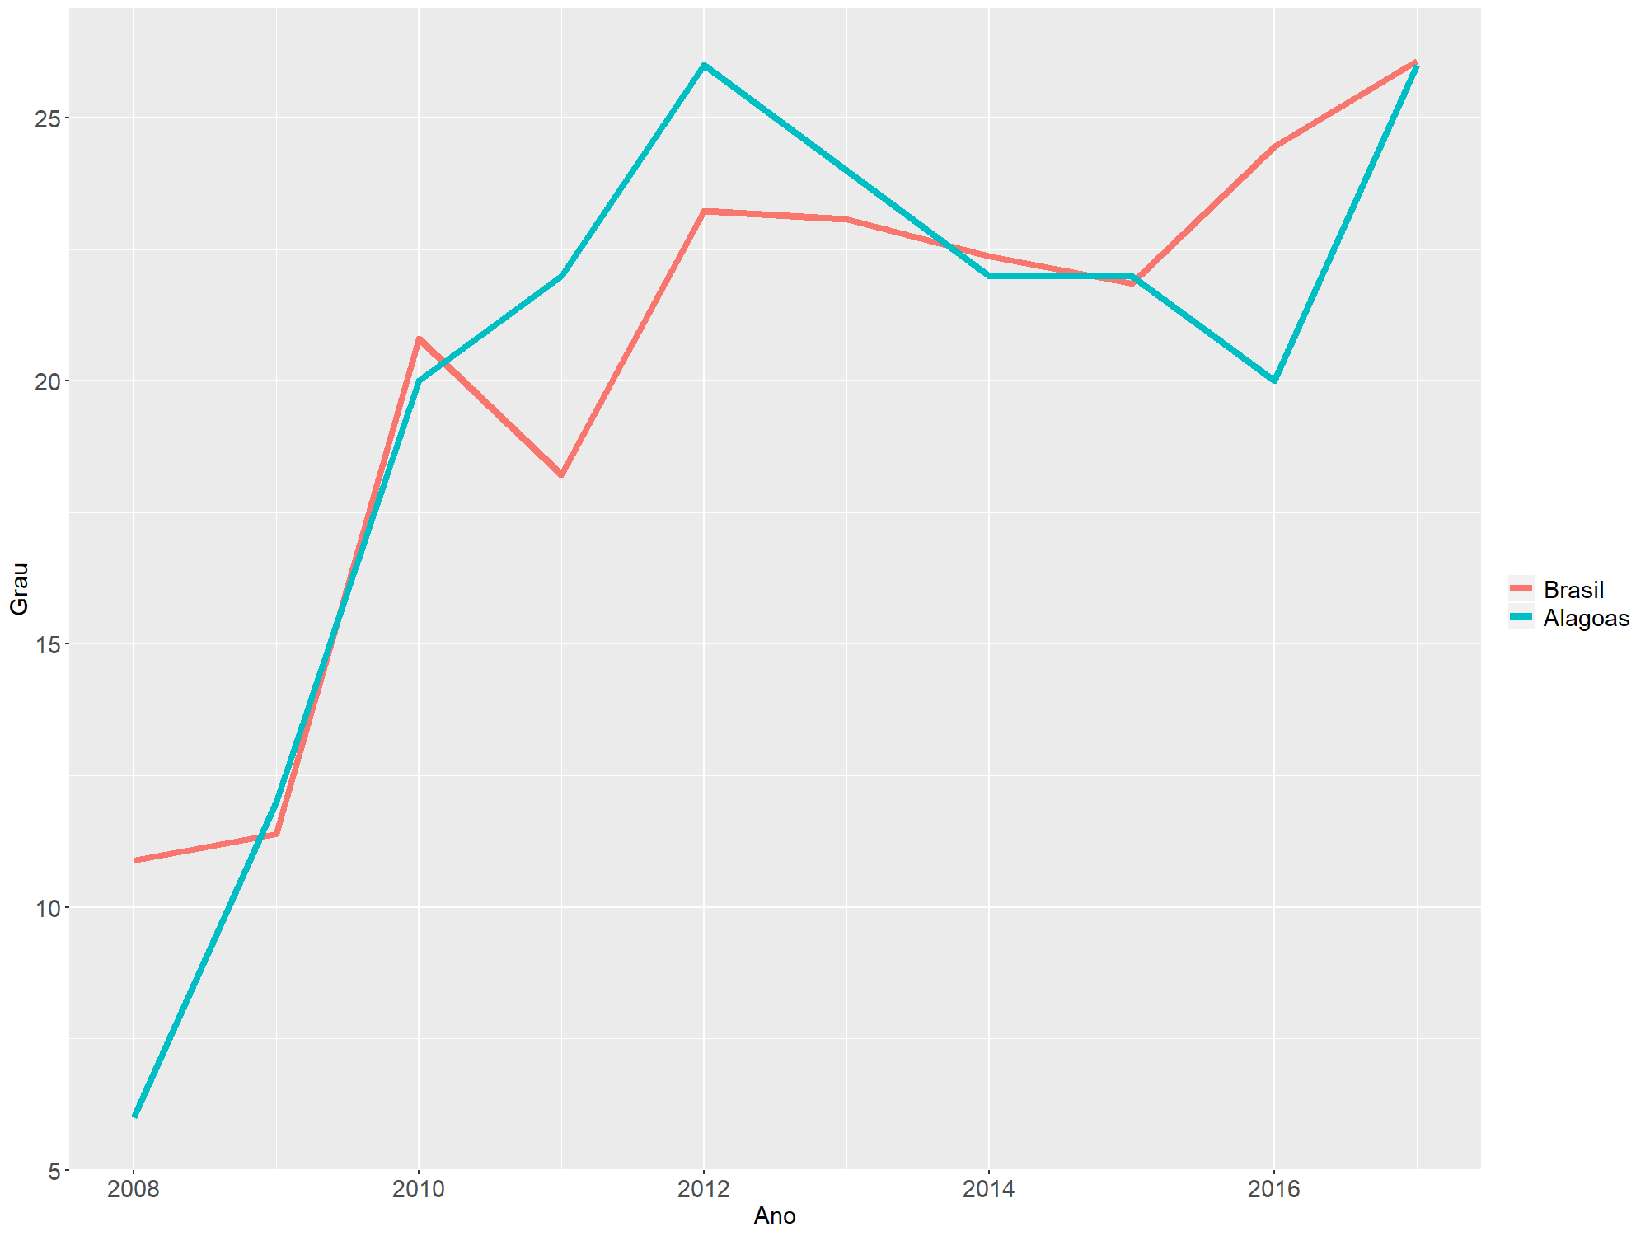
\includegraphics[scale=0.4]{Imagens/agricultural/graf-linha-degree-br-al.pdf}
	\caption{Centralidade do Grau (\textit{Agricultural Sciences})}
	\label{degree-agri-1}
\end{figure}

\subsubsection{Exact and Earth Sciences}

\begin{figure}[H]
	\centering
	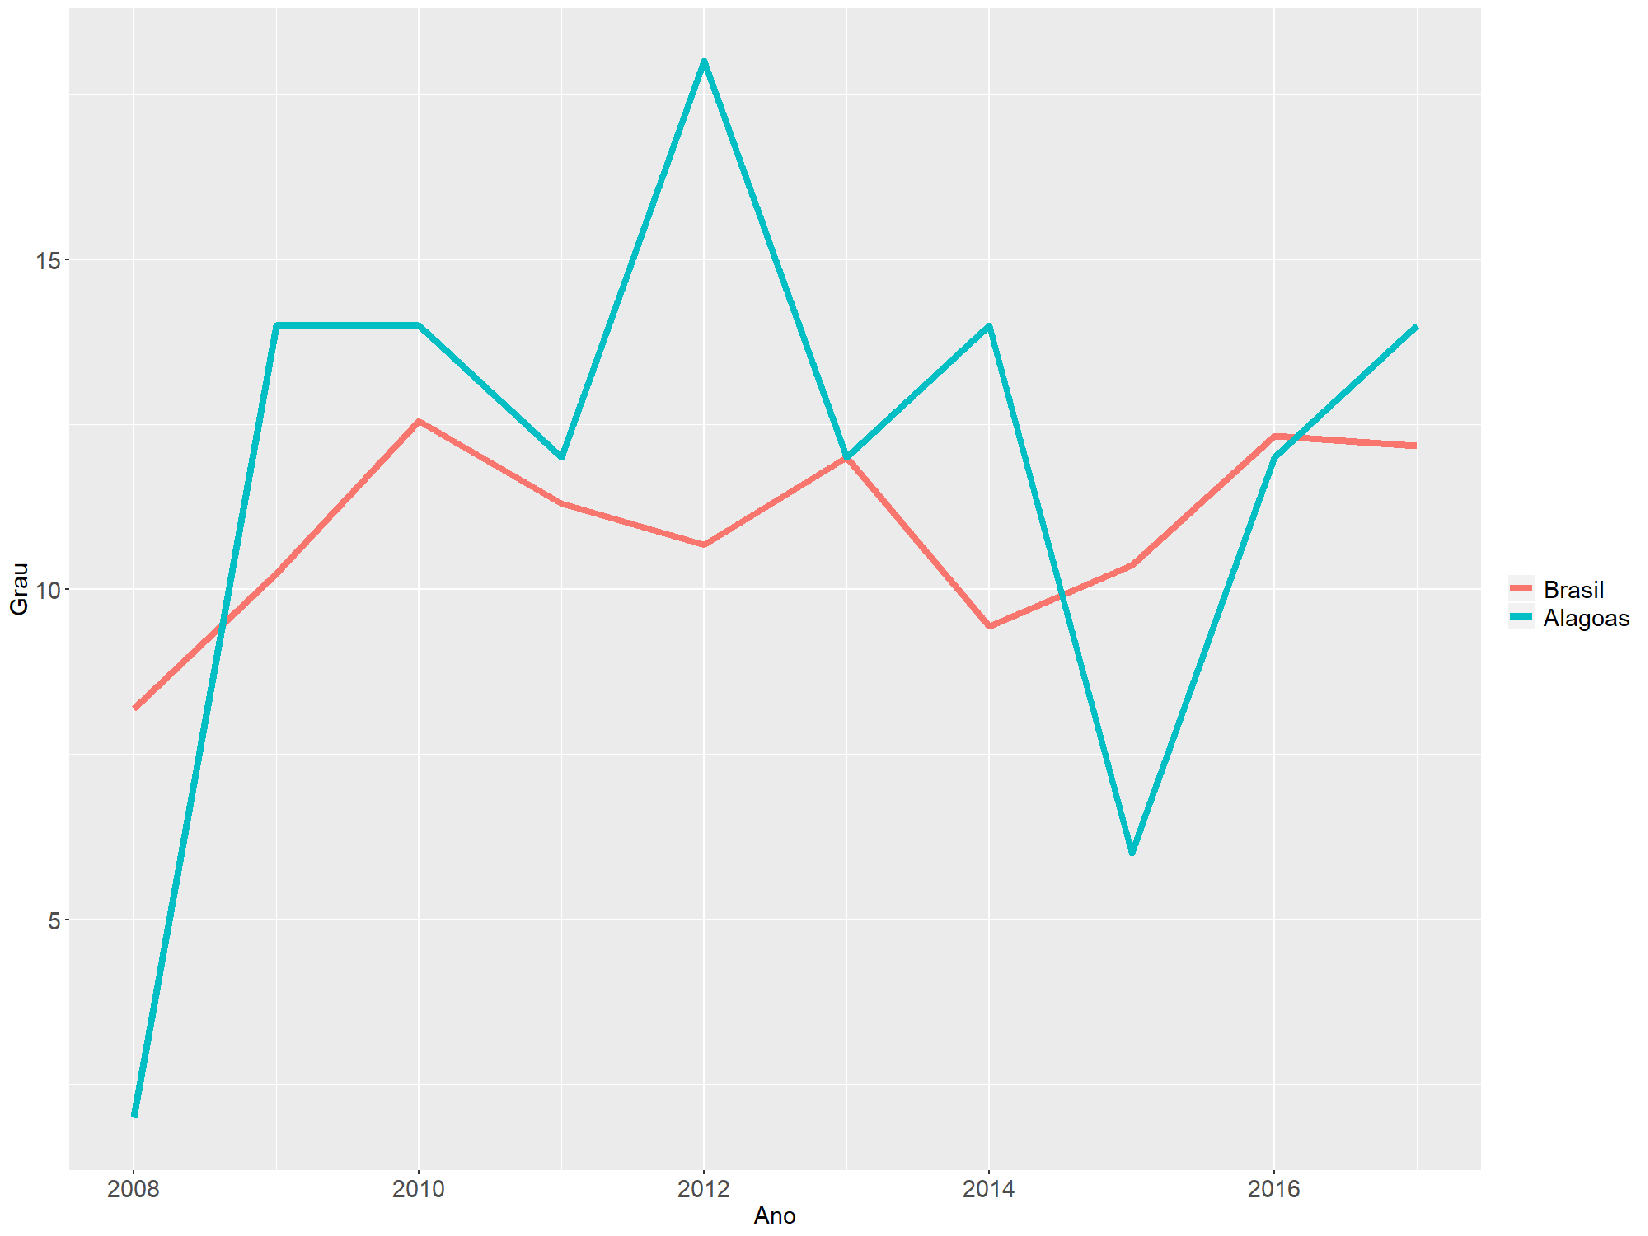
\includegraphics[scale=0.4]{Imagens/exact/graf-linha-degree-br-al.pdf}
	\caption{Centralidade do Grau (\textit{Exact and Earth Sciences})}
	\label{degree-exact-1}
\end{figure}

Os gráficos \ref{degree-health-1}, \ref{degree-agri-1} e \ref{degree-exact-1}, apresentam respectivamente as curvas na série temporal (2008-2017) da centralidade do grau da média da Rede Brasil e Alagoas. 

Na disposição das curvas na área de \textit{Health Sciences}, sendo Rede Brasil (vermelha) e Alagoas (azul), percebemos ao longo do período projeção em direção análoga, e que exceto como aferido no ano de 2009 e 2011, Alagoas esteve com a centralidade do grau maior que a média do Brasil. O que nos levar a inferir que nesse período

O gráfico \ref{degree-agri-1} mostra que Alagoas andou muito próximo da média do Brasil para \textit{Agricultural Sciences} para este indicador. Destaque para o ano de 2012, em que obteve o maior índice de centralidade na rede, estas razões podem ser investigadas com maior detalhamento sobre as ocorrências das coautorias neste ano.

A análise da centralidae para área de \textit{Exact and Earth Sciences} mostra que apesar de não ser uma área de grande volume de artigos indexados na base SciELO, a partir de 2009, Alagoas obteve um índice de centralidade maior que a média da rede. Com um queda considerável do seu índice em 2015, como dito uma análise investigatória poderá responder o que ocorreu neste ano, como a desconexão com outros vértices, não ocorrendo coautorias em pares com outros estados.

%% HISTOGRAMAS GRAU

\begin{figure}[H]
	\centering
	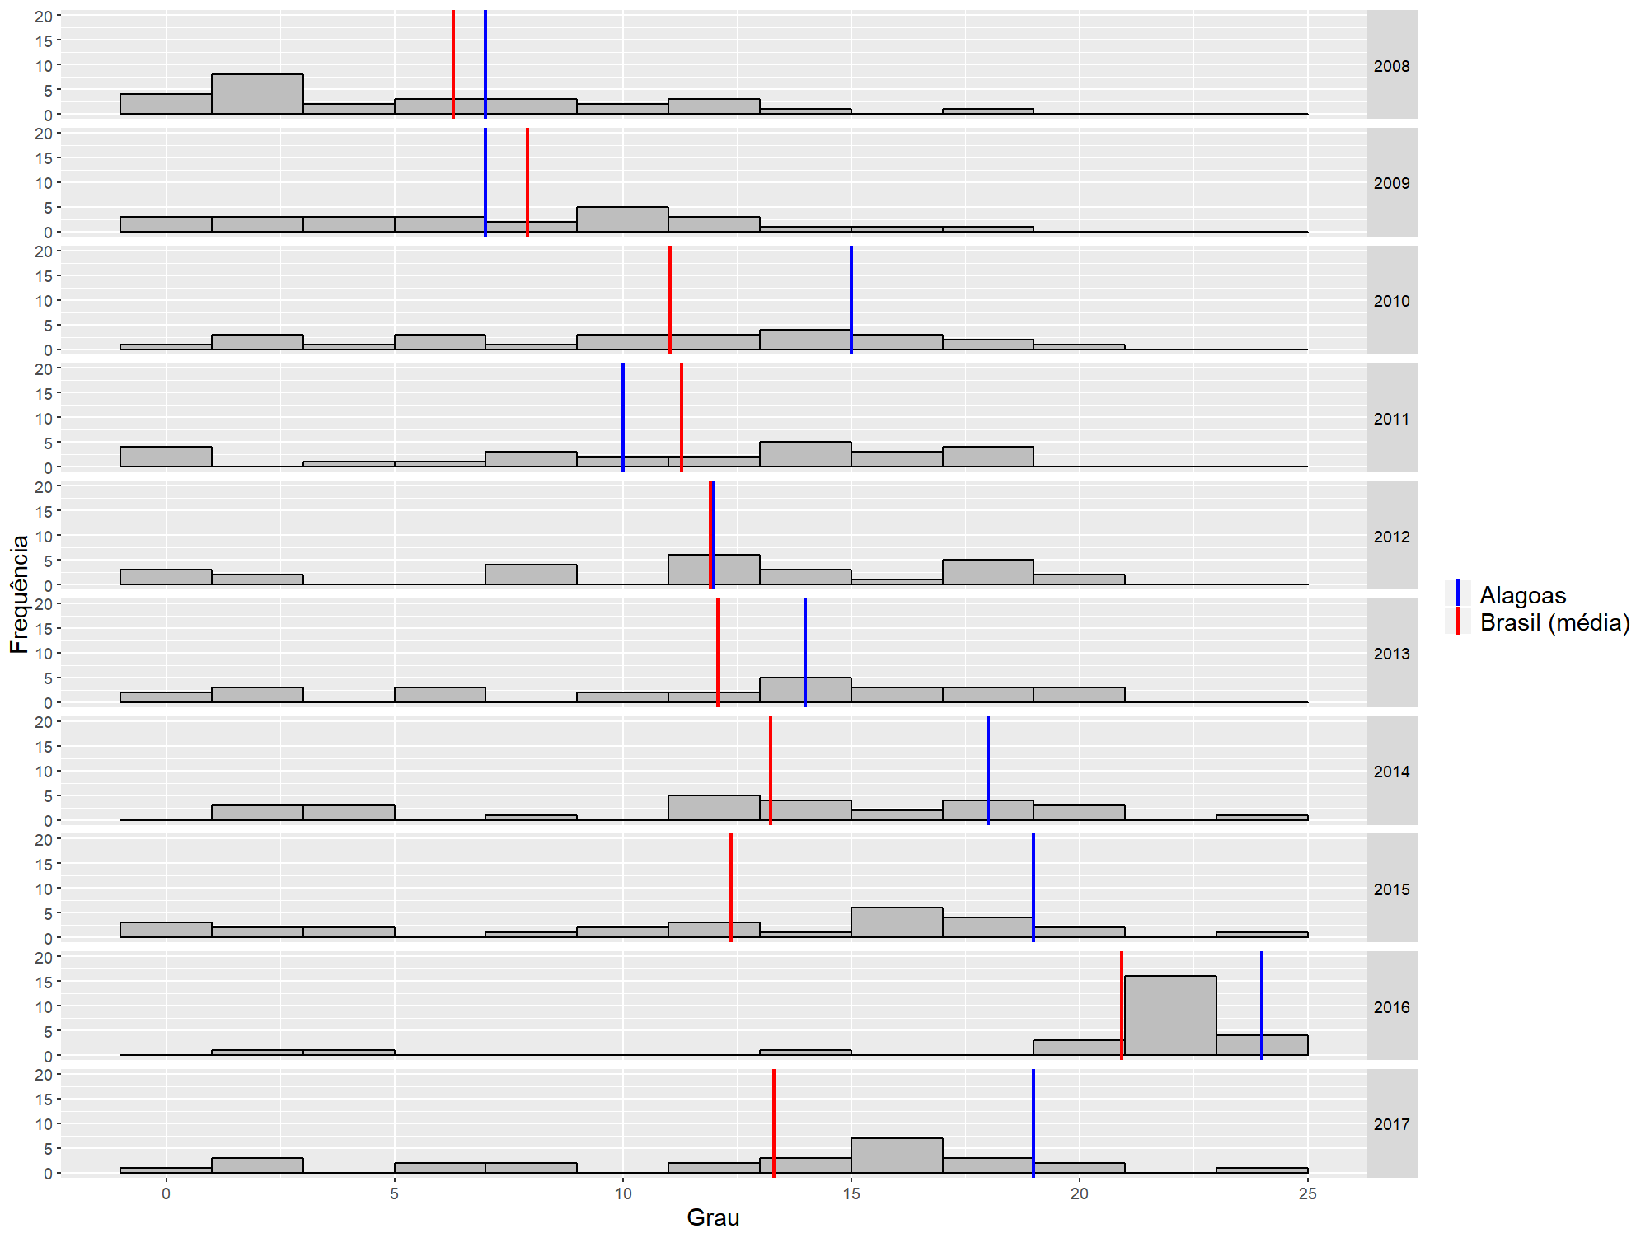
\includegraphics[scale=0.5]{Imagens/degree-hist.pdf}
	\caption{Histograma da Centralidade do Grau (\textit{Health Sciences})}
	\label{degree-health-hist-1}
\end{figure}

\begin{figure}[H]
	\centering
	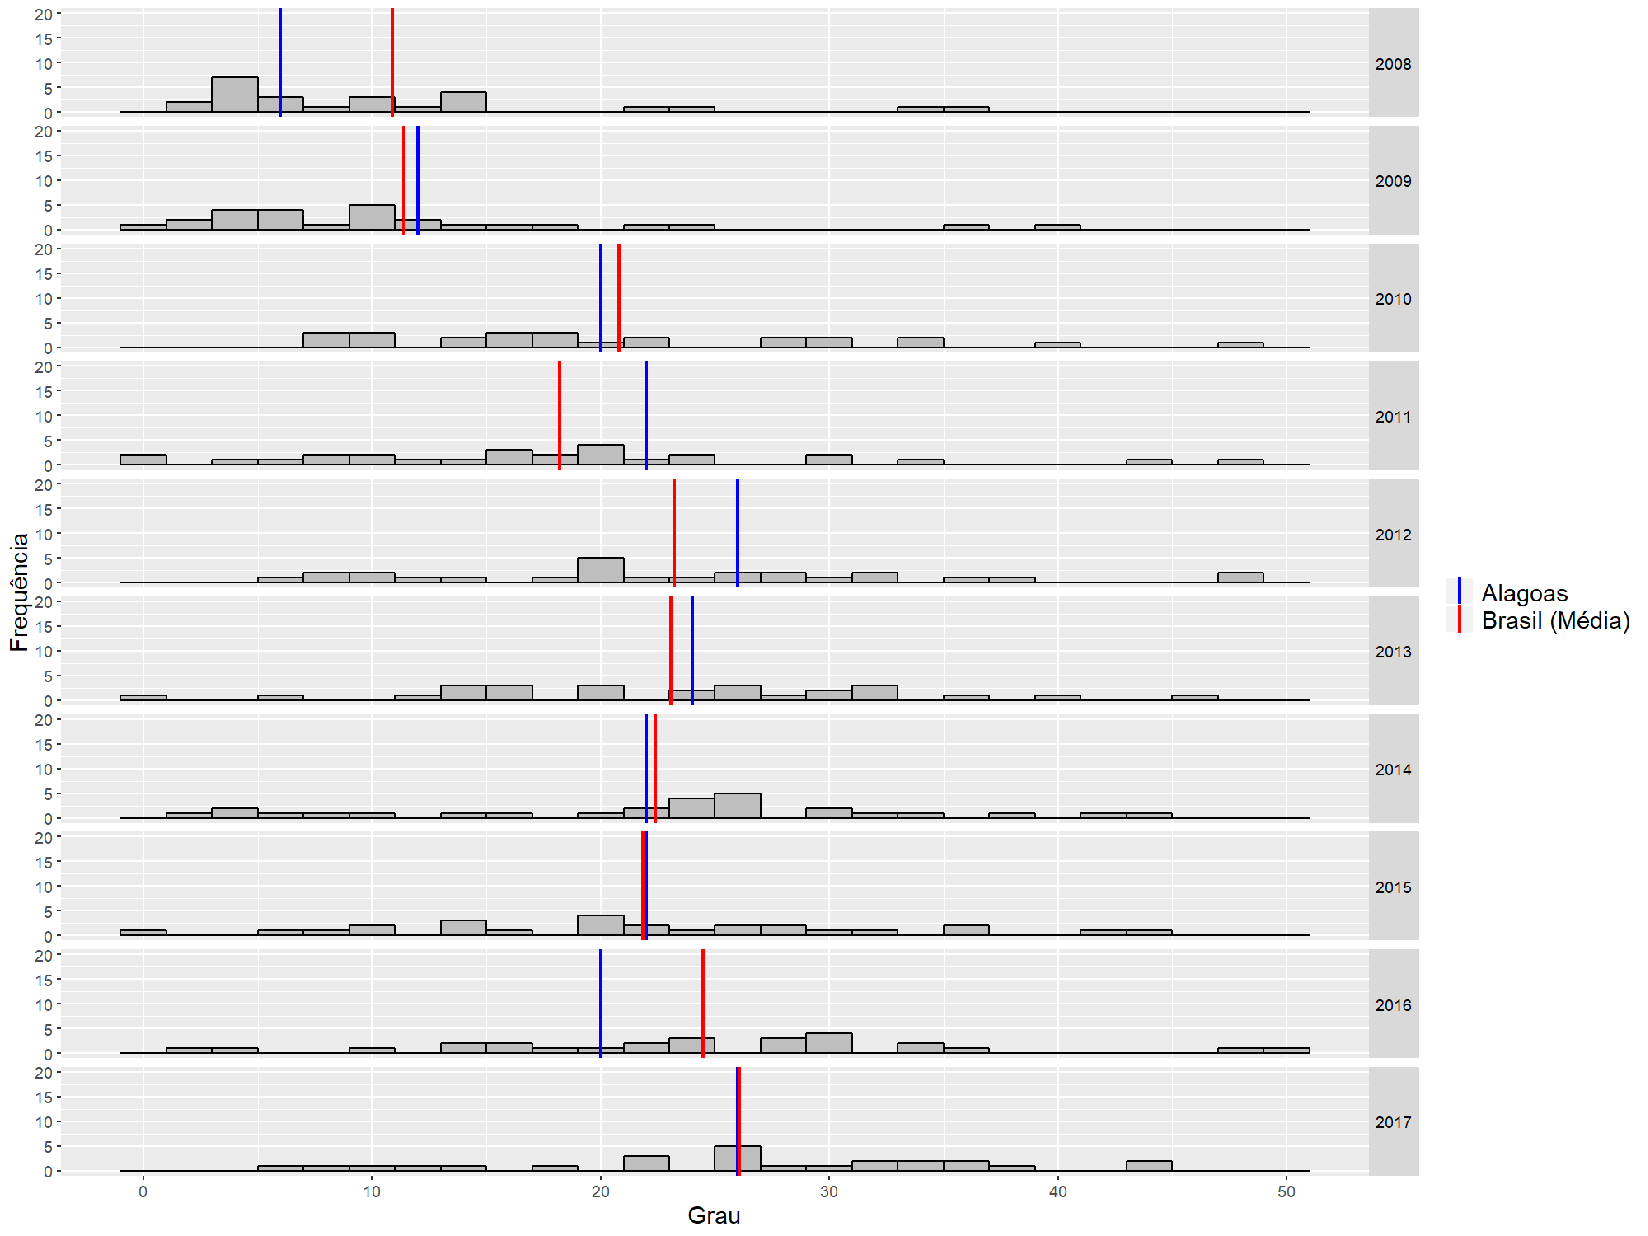
\includegraphics[scale=0.5]{Imagens/agricultural/degree-hist.pdf}
	\caption{Histograma da Centralidade do Grau (\textit{Agricultural Sciences})}
	\label{degree-agri-hist-1}
\end{figure}

\begin{figure}[H]
	\centering
	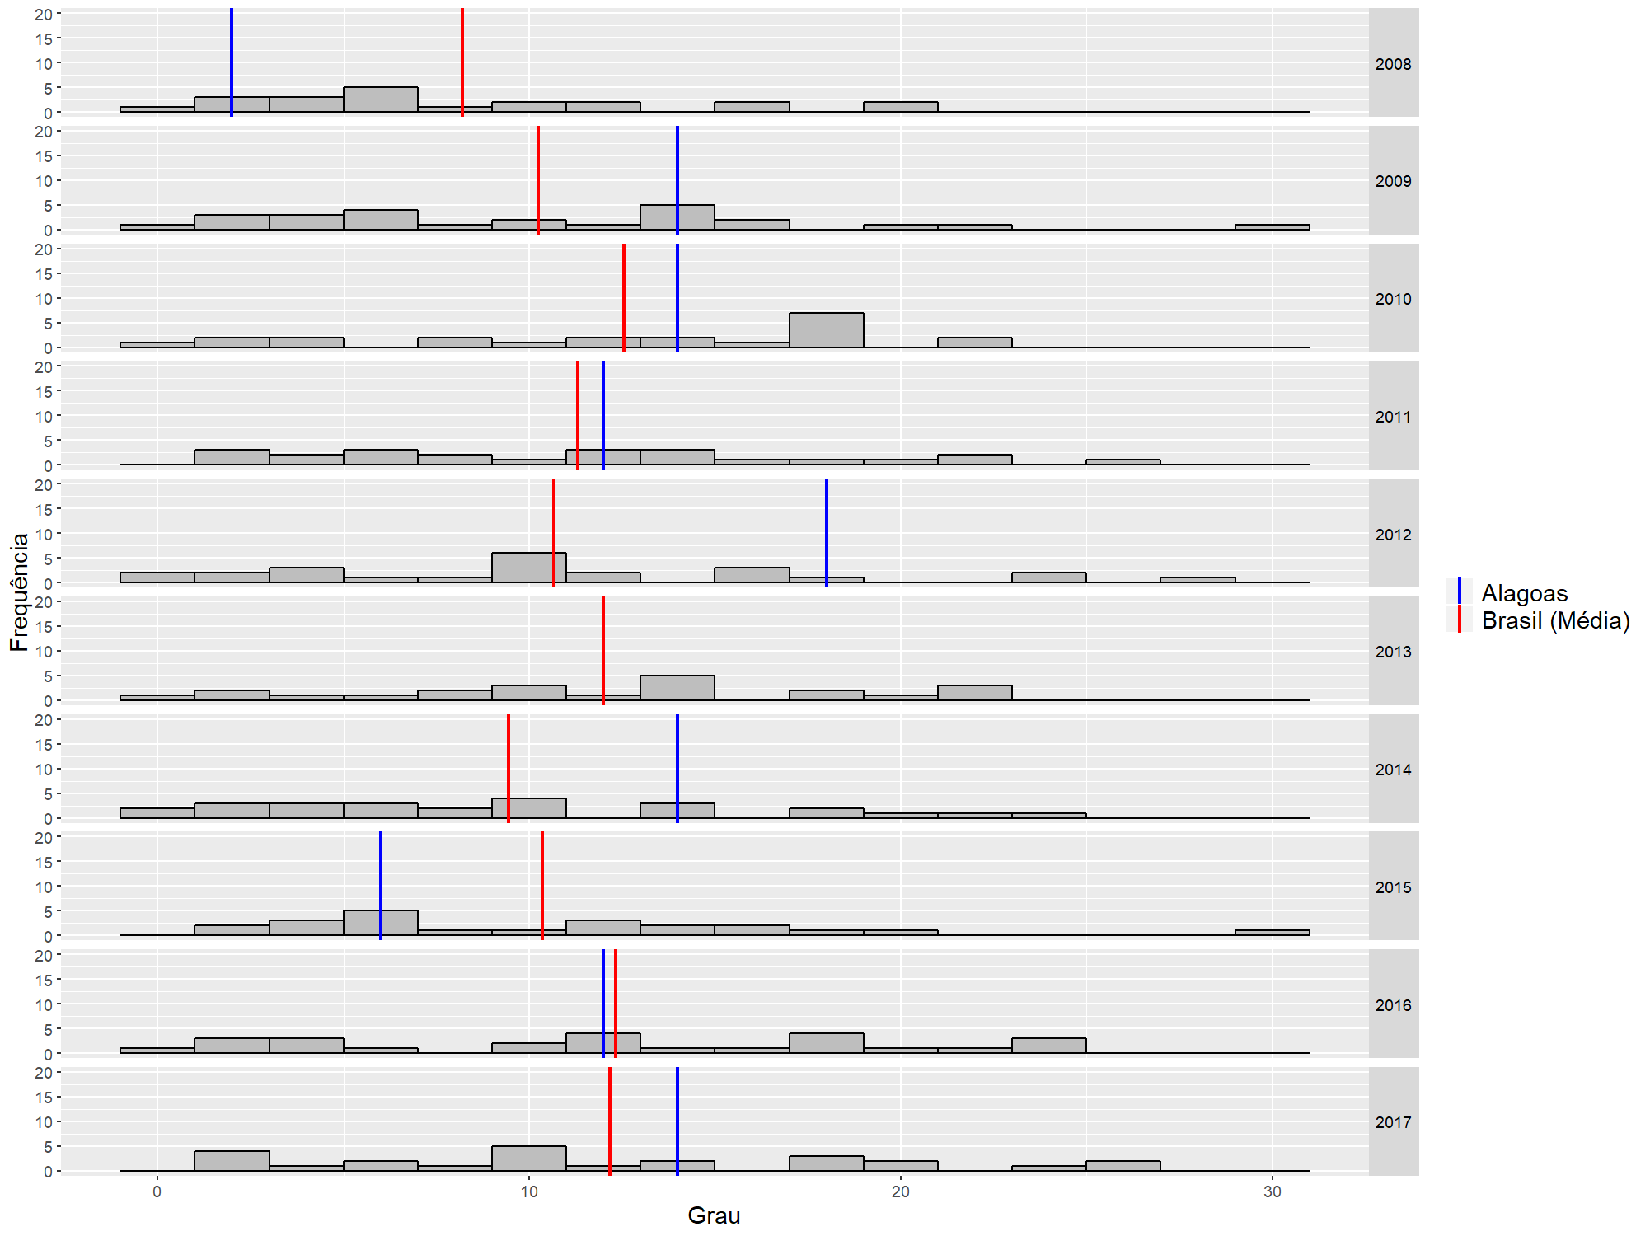
\includegraphics[scale=0.5]{Imagens/exact/degree-hist.pdf}
	\caption{Histograma da Centralidade do Grau (\textit{Exact and Earth Sciences})}
	\label{degree-exact-hist-1}
\end{figure}


O histograma \ref{degree-health-hist-1} indica a distribuição da medida de centralidade do grau para área de \textit{Health Sciences}, maneira a qual percebemos uma grande frequência no ano de 2016, em virtude da clusterização observada na tabela \ref{estruturais}, corroborando os anos que Alagoas (linha azul) esteve a frente neste marcador quando comparado a média do Brasil.

Na figura \ref{degree-agri-hist-1} observamos um posicionamento muito próximo da média da Rede Brasil (linha vermelha) e Alagoas (linha azul), e que exceto nos primeiro anos de 2008 a 2009 a distribuição concentrou-se na região central, de forma que muitos vértices obtiveram índices parecidos, exceto \textit{outliers} que estão presente em cada ano, dos quais podemos verificar na matriz \ref{matriz-agri} e no ranking apresentando em seção abaixo.

O histograma, figura \ref{degree-exact-hist-1} da área de \textit{Exact and Earth Sciences} mostra o posicionamento da centralidade do grau de Alagoas acima do Brasil, e uma distribuição dos índices aferidos mais dispersos.

%%% CLOSENESS

\subsection{\textbf{Centralidade de Proximidade}}

A figura \ref{closeness-tab} apresenta os resultados da medida de centralidade de proximidade em relação a Rede Brasil (média) e Alagoas, para todas as áreas. Essa medida indica quão próximo um vértice encontra-se um do outro, considerando seu posicionamento na rede. Indicando assim o seu papel de influência e importância pelo aspecto da proximidade.


\begin{table}[H]
	\centering
	\begin{tabular}{|c|l|l|l|l|l|l|}
		\hline
		\multicolumn{7}{|c|}{\textbf{\begin{tabular}[c]{@{}c@{}}Centralidade de Proximidade  \\ (Closeness Centrality) por Área\end{tabular}}}                                                                                                                                                                                                                                                  \\ \hline
		\rowcolor[HTML]{C0C0C0} 
		\textbf{Ano}    & \multicolumn{2}{|c|}{\cellcolor[HTML]{C0C0C0}\textbf{\begin{tabular}[c]{@{}c@{}}Health \\ Sciences\end{tabular}}} & \multicolumn{2}{|c|}{\cellcolor[HTML]{C0C0C0}\textbf{\begin{tabular}[c]{@{}c@{}}Agricultural \\ Sciences\end{tabular}}} & \multicolumn{2}{c|}{\cellcolor[HTML]{C0C0C0}\textbf{\begin{tabular}[c]{@{}c@{}}Exact and \\ Earth Sciences\end{tabular}}} \\ \hline
		\rowcolor[HTML]{EFEFEF} 
		\textbf{Rede}   & \textbf{Brasil}                                        & \textbf{Alagoas}                                        & \textbf{Brasil}                                           & \textbf{Alagoas}                                           & \textbf{Brasil}                                             & \textbf{Alagoas}                                            \\ \hline
		2008            & 0,5303                                                 & 0,5434                                                  & 0,5414                                                    & 0,4528                                                     & 0,4824                                                      & 0,3333                                                      \\ \hline
		2009            & 0,5789                                                 & 0,5609                                                  & 0,5543                                                    & 0,5455                                                     & 0,4978                                                      & 0,5610                                                       \\ \hline
		2010            & 0,6772                                                 & 0,7419                                                  & 0,6531                                                    & 0,6316                                                     & 0,5435                                                      & 0,5263                                                      \\ \hline
		2011            & 0,6699                                                 & 0,6216                                                  & 0,6444                                                    & 0,6487                                                     & 0,5216                                                      & 0,5366                                                      \\ \hline
		2012            & 0,6700                                                   & 0,6666                                                  & 0,6663                                                    & 0,6757                                                     & 0,5400                                                        & 0,6000                                                         \\ \hline
		2013            & 0,6852                                                 & 0,7058                                                  & 0,6747                                                    & 0,6667                                                     & 0,5544                                                      & 0,5556                                                      \\ \hline
		2014            & 0,6957                                                 & 0,7812                                                  & 0,6312                                                    & 0,6191                                                     & 0,5033                                                      & 0,5641                                                      \\ \hline
		2015            & 0,6697                                                 & 0,7812                                                  & 0,6676                                                    & 0,6487                                                     & 0,5306                                                      & 0,5122                                                      \\ \hline
		2016            & 0,8788                                                 & 0,9615                                                  & 0,6780                                                     & 0,6250                                                      & 0,5206                                                      & 0,5111                                                      \\ \hline
		2017            & 0,6993                                                 & 0,8064                                                  & 0,6995                                                    & 0,6857                                                     & 0,5267                                                      & 0,5750                                                       \\ \hline
	\end{tabular}
\caption{Medidas de Centralidade de Proximidade por Área (2008-2017)}
\label{closeness-tab}
\end{table}


\subsubsection{Health Sciences}

\begin{figure}[H]
	\centering
	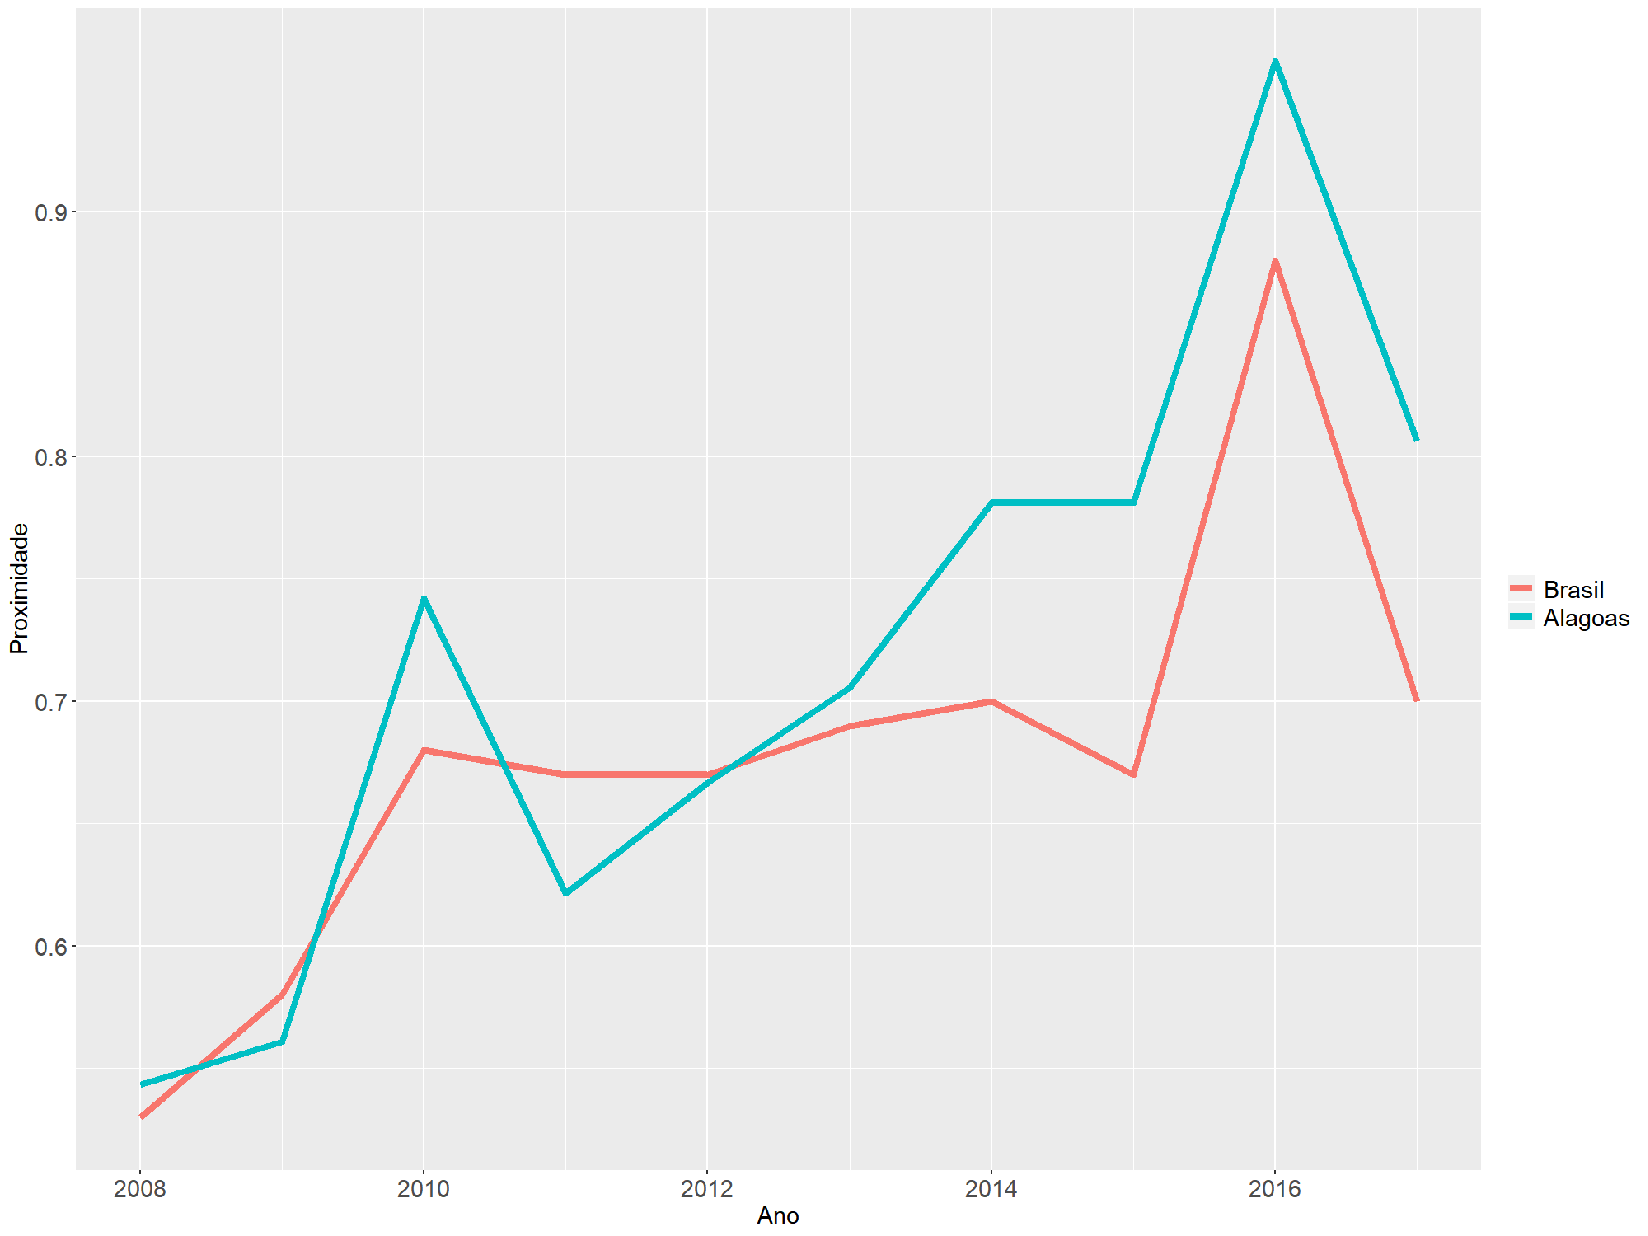
\includegraphics[scale=0.4]{Imagens/graf-linha-closeness-br-al.pdf}
	\caption{Centralidade de Proximidade (\textit{Health Sciences})}
	\label{close-health-1}
\end{figure}

\subsubsection{Agricultural Sciences}

\begin{figure}[H]
	\centering
	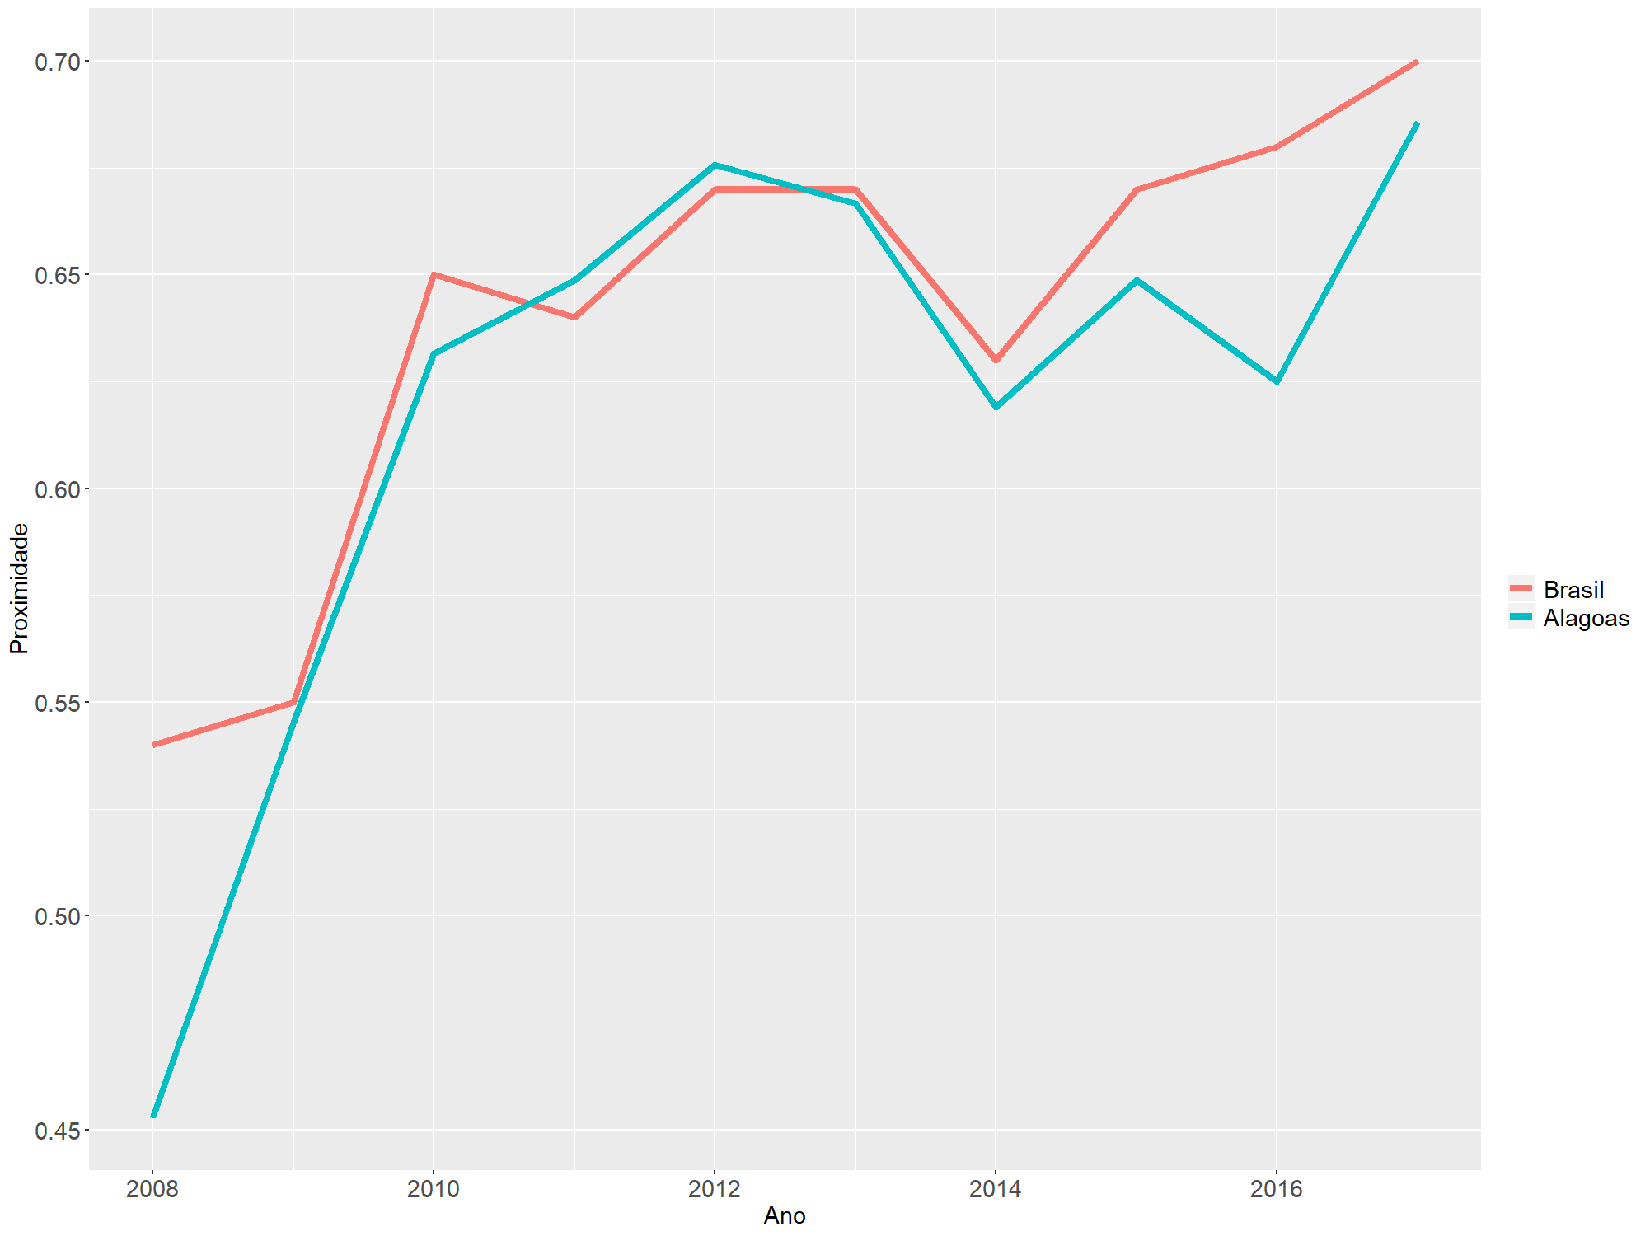
\includegraphics[scale=0.4]{Imagens/agricultural/graf-linha-closeness-br-al.pdf}
	\caption{Centralidade de Proximidade (\textit{Agricultural Sciences})}
	\label{close-agri-1}
\end{figure}

\subsubsection{Exact and Earth Sciences}

\begin{figure}[H]
	\centering
	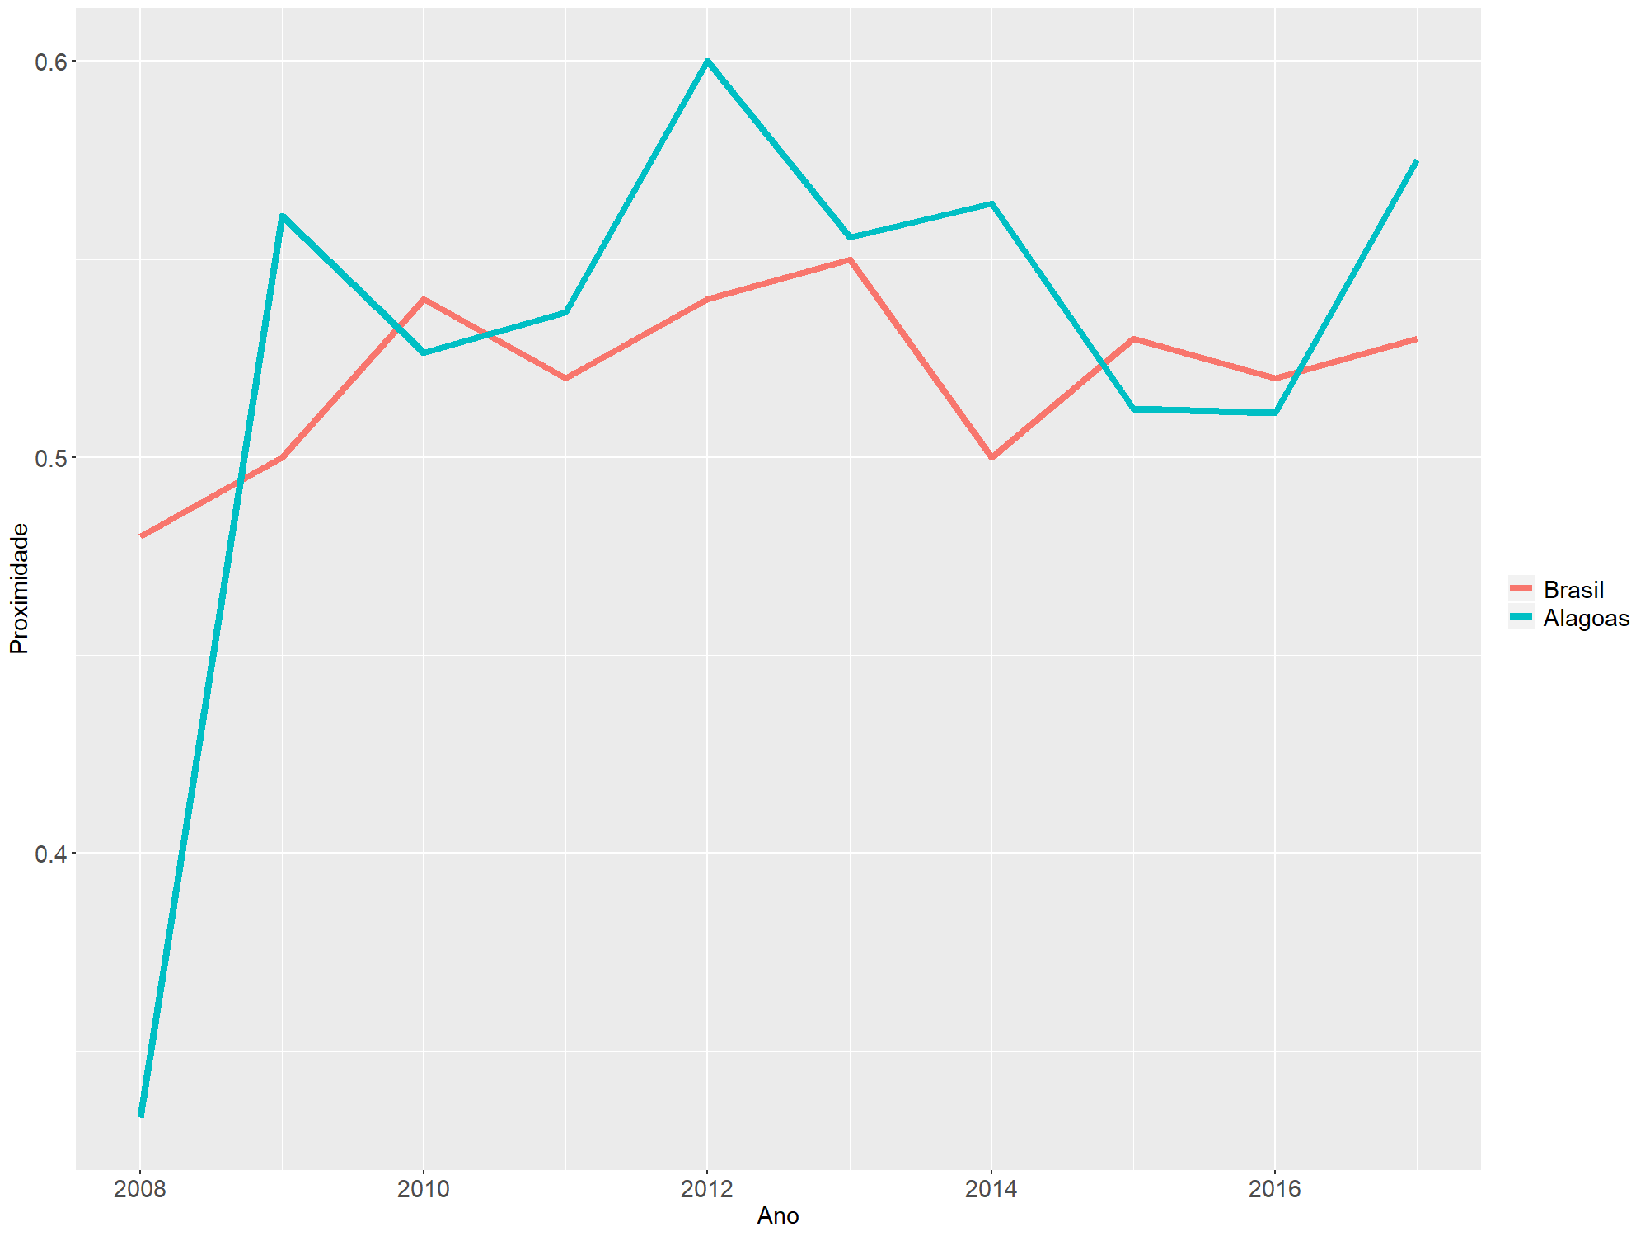
\includegraphics[scale=0.4]{Imagens/exact/graf-linha-closeness-br-al.pdf}
	\caption{Centralidade de Proximidade (\textit{Exact and Earth Sciences})}
	\label{close-exact-1}
\end{figure}

As curvas da Rede Brasil (vermelha) e Alagoas (azul), também se projetaram em sentidos análogos, destaque que na área de \textit{Health Sciences} conforme \ref{close-health-1} que exceto nos anos 2009 e 2011 em todo o período manteve-se acima da média do Brasil. 

Na área de \textit{Agricultural Science} conforme figura \ref{close-agri-1}, os resultados foram muito próximos, resultando que Alagoas ficou em que alguns anos abaixo da média, como vimos na figura da Matriz de Coautoria \ref{matriz-agri} e o que será corroborado pelo ranking apresentado abaixo, pelo destaque dos estados do Rio Grande do Sul e Rio Grande do Norte em Ciências Agrárias.

Na análise gráfica da centralidade de proximidade da área \textit{Exact and Earth Sciences}, verificamos um baixo índice aferido por Alagoas no ano de 2008 e que a partir de 2009 seguiu em patamar superior a média do Brasil, tendo sido a área de maior destaque para medidade de centralidade da proximidade.


\subsubsection{Health Sciences}

\begin{figure}[H]
	\centering
	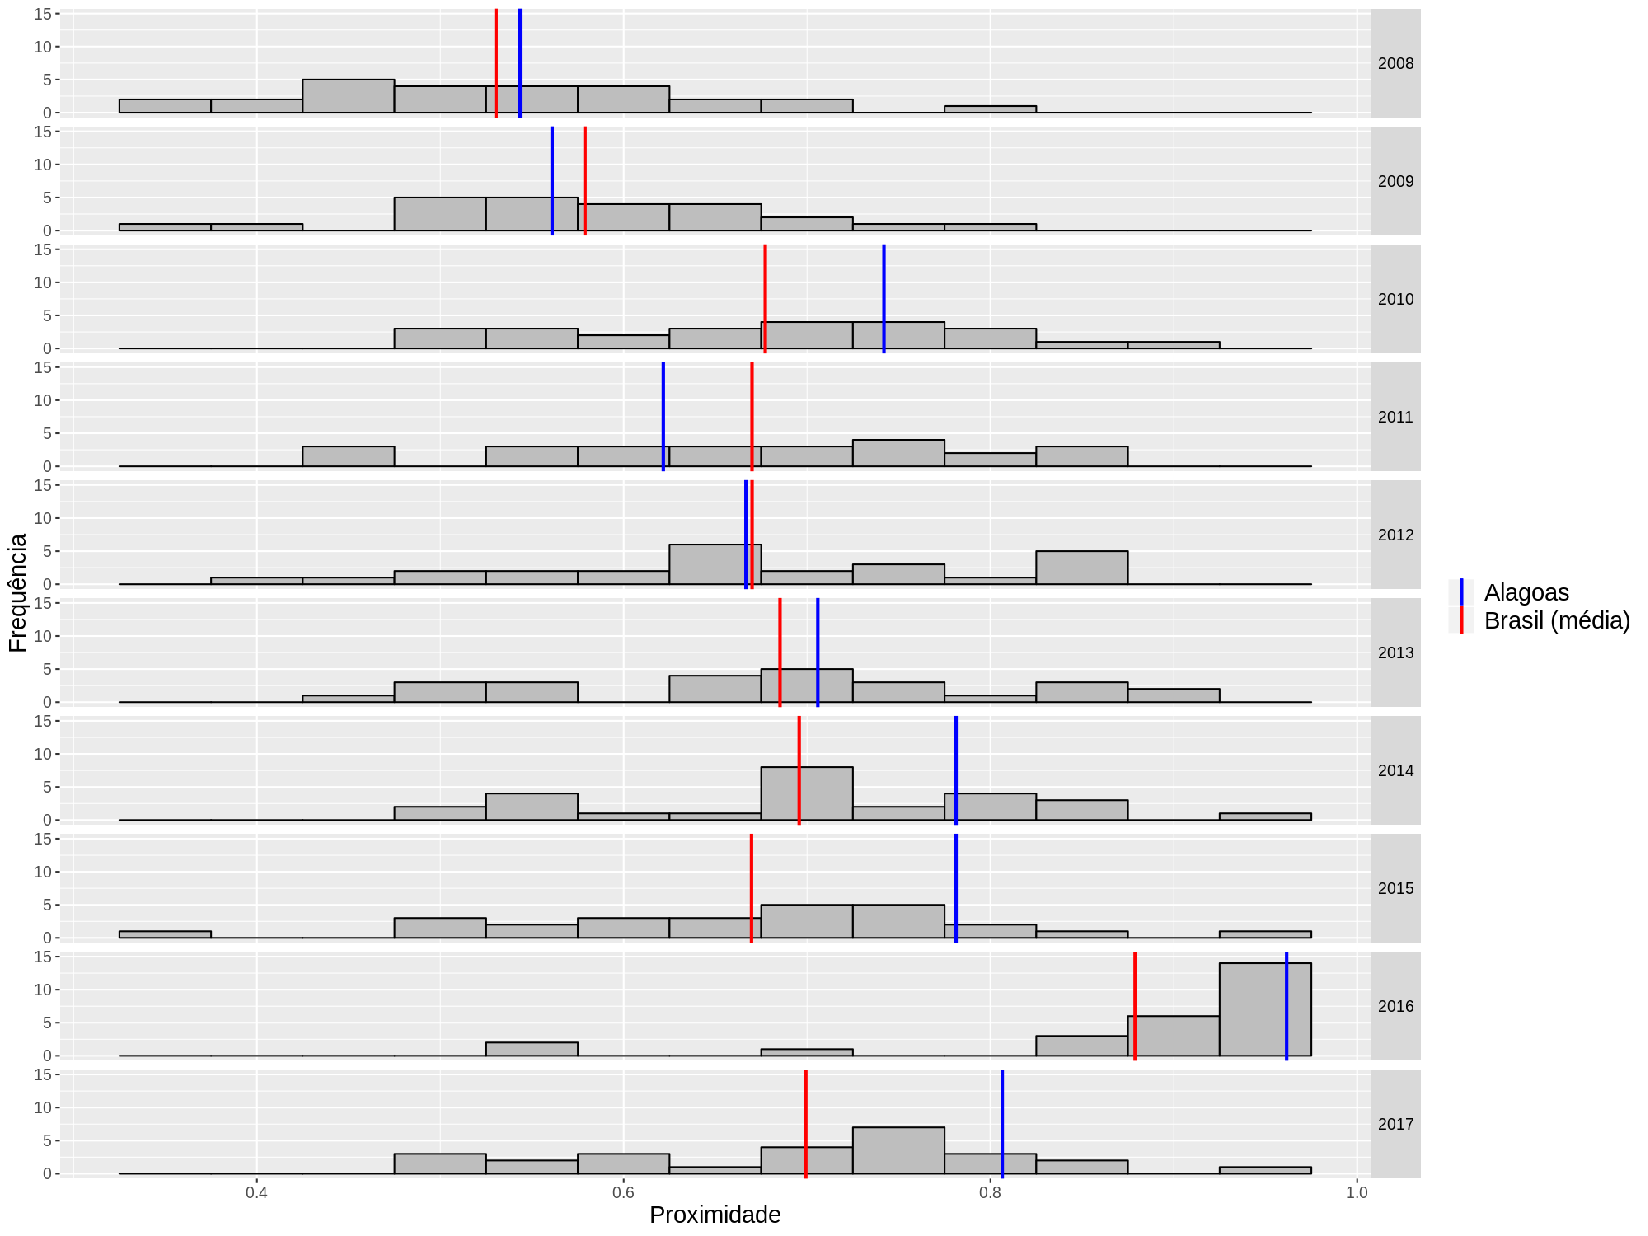
\includegraphics[scale=0.5]{Imagens/closeness-hist.pdf}
	\caption{Histograma da Centralidade de Proximidade (\textit{Health Sciences})}
	\label{hist-health-close-1}
\end{figure}

\subsubsection{Agricultural Sciences}

\begin{figure}[H]
	\centering
	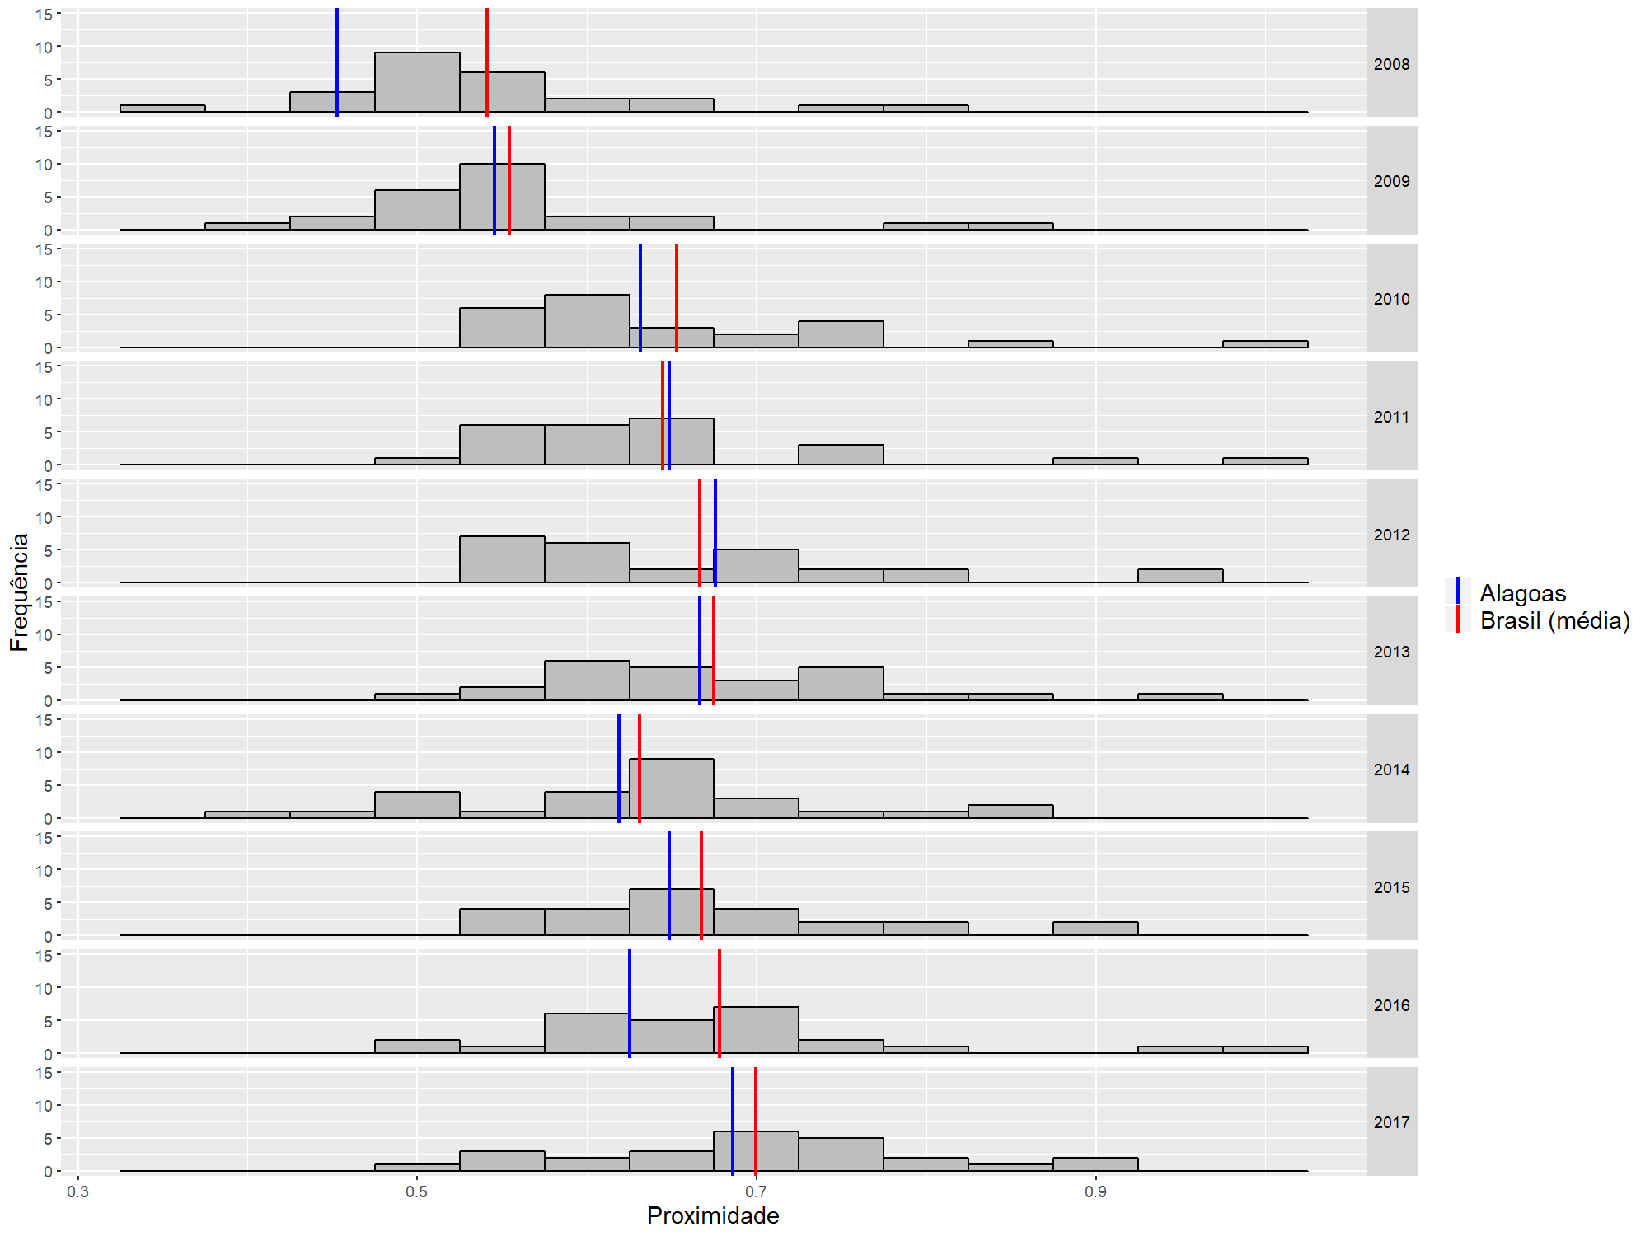
\includegraphics[scale=0.5]{Imagens/agricultural/closeness-hist.pdf}
	\caption{Histograma da Centralidade de Proximidade (\textit{Agricultural Sciences})}
	\label{hist-agri-close-1}
\end{figure}

\subsubsection{Exact and Earth Sciences}

\begin{figure}[H]
	\centering
	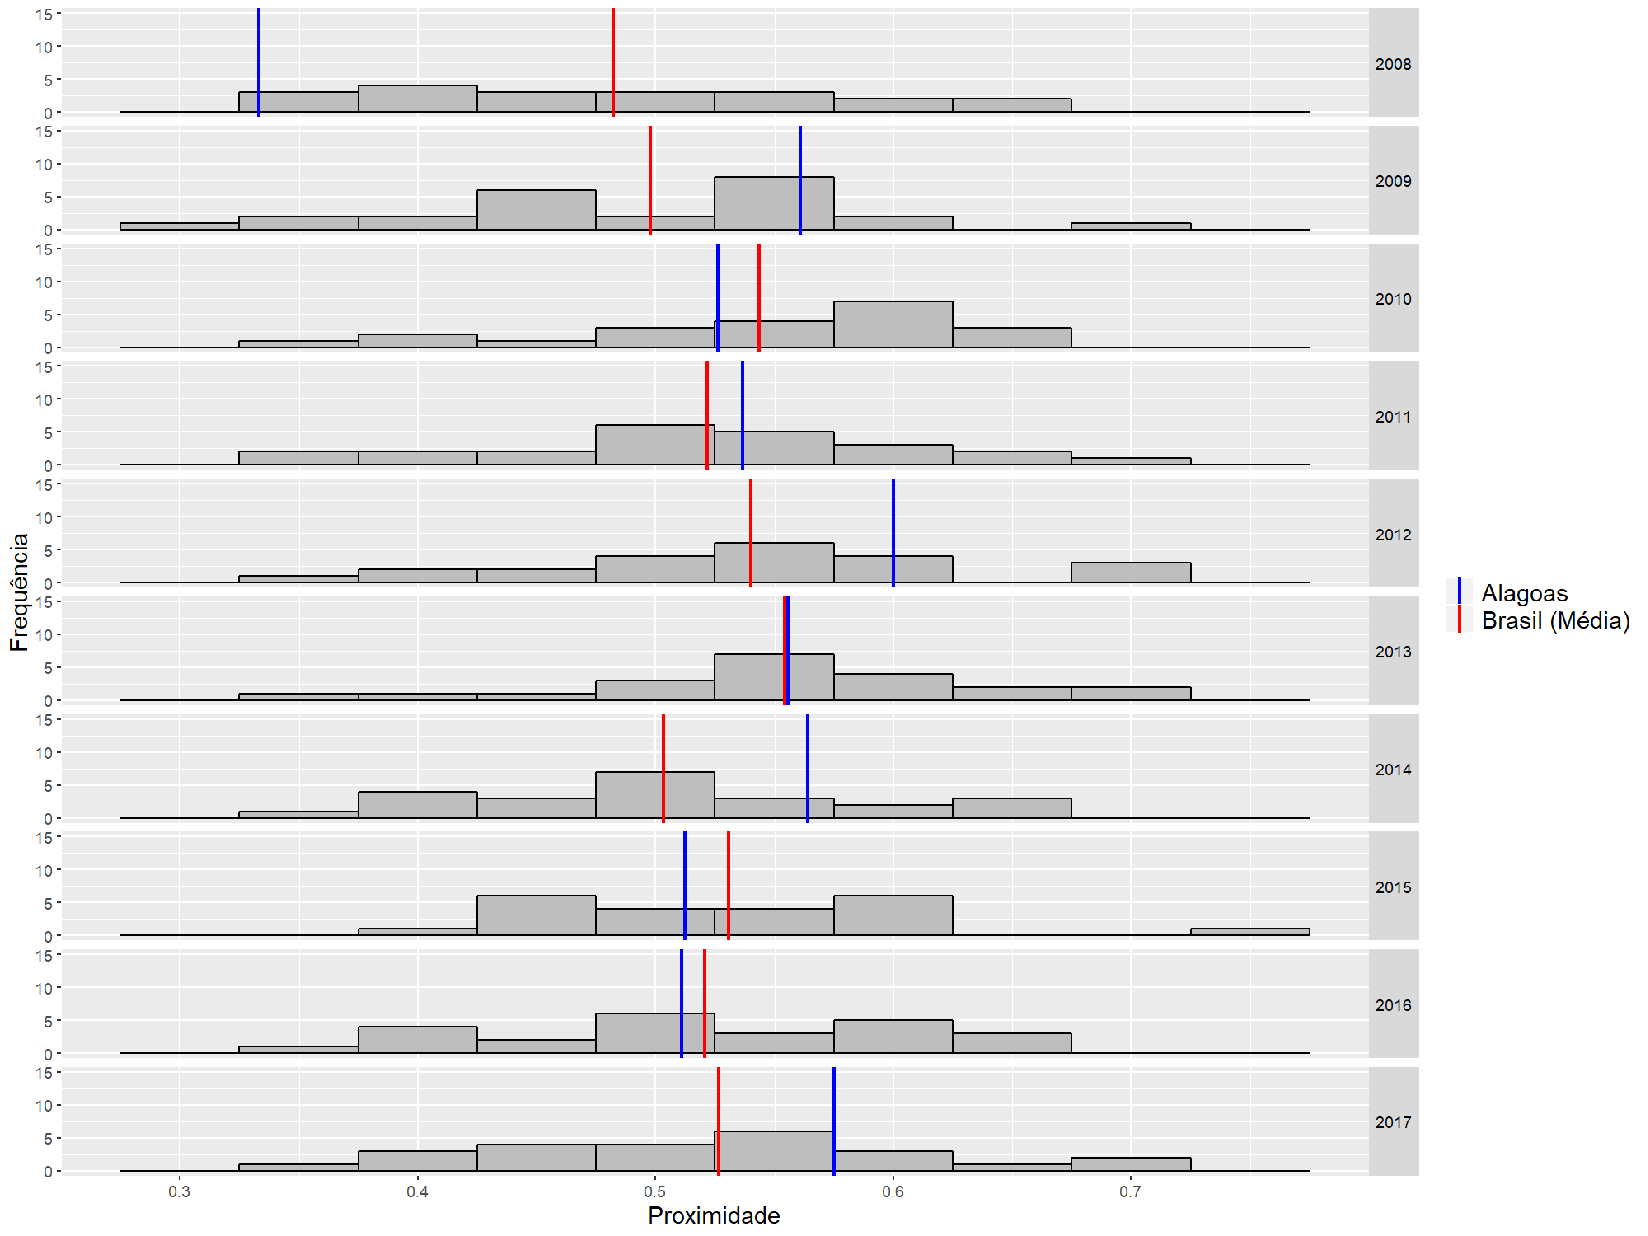
\includegraphics[scale=0.5]{Imagens/exact/closeness-hist.pdf}
	\caption{Histograma da Centralidade de Proximidade (\textit{Exact and Earth Sciences})}
	\label{hist-exact-close-1}
\end{figure}

As figuras \ref{hist-health-close-1}, apresenta o histograma de distribuição para a área de \textit{Health Sciences}, o qual podemos destacar ano de 2016, em que as frequências se concentraram em alto índice comparado aos demais anos, e que Alagoas ficou acima da média para essa medida desde o ano de 2013. Resultando que sua proximidade quando comparada a média dos vértices do Brasil é superior.

Em \textit{Agricultural Sciences}, visto pelo histograma na figura \ref{hist-agri-close-1}, a média do Brasil e Alagoas são marcados muito próximos no histograma que possui distribuição em todos anos muito central. De forma que esta medida não apresentou relevante informação nessa área.

O histograma \ref{hist-exact-close-1} apresenta uma distribuição de sua frequência mais espaçada, sendo observador o marcador de Alagoas muito baixo no ano de 2008, muito provável pelos poucos artigos indexados neste ano por autores Alagoanos na área de \textit{Exact and Earth Sciences}, mas que a partir de 2009 a proximidade de Alagoas com a média do Brasil, supera em 2011, 2012, 2014, e 2017,


%%% BETWEENESS

\subsection{\textbf{Centralidade de Intermediação}}

A figura \ref{betweeness-tab} apresenta os resultados da medida de centralidade de intermediação em relação a Rede Brasil (média) e Alagoas, para todas as áreas. Essa medida indica a capacidade de intermediação de um vértice a outro, considerando seu posicionamento na rede.

\begin{table}[H]
	\centering
	\begin{tabular}{|c|l|l|l|l|l|l|}
		\hline
		\multicolumn{7}{|c|}{\textbf{\begin{tabular}[c]{@{}c@{}}Centralidade de Intermediação\\ (Betweeness Centrality) por Área\end{tabular}}}                                                                                                                                                                                                                                                 \\ \hline
		\rowcolor[HTML]{C0C0C0} 
		\textbf{Ano}    & \multicolumn{2}{c|}{\cellcolor[HTML]{C0C0C0}\textbf{\begin{tabular}[c]{@{}c@{}}Health \\ Sciences\end{tabular}}} & \multicolumn{2}{c|}{\cellcolor[HTML]{C0C0C0}\textbf{\begin{tabular}[c]{@{}c@{}}Agricultural \\ Sciences\end{tabular}}} & \multicolumn{2}{c|}{\cellcolor[HTML]{C0C0C0}\textbf{\begin{tabular}[c]{@{}c@{}}Exact and \\ Earth Sciences\end{tabular}}} \\ \hline
		\rowcolor[HTML]{EFEFEF} 
		\textbf{Rede}   & \textbf{Brasil}                                        & \textbf{Alagoas}                                        & \textbf{Brasil}                                            & \textbf{Alagoas}                                          & \textbf{Brasil}                                             & \textbf{Alagoas}                                            \\ \hline
		2008            & 0,0370                                                  & 0,0100                                                    & 0,0400                                                       & 0,0047                                                    & 0,0476                                                      & 0,0021                                                      \\ \hline
		2009            & 0,0396                                                 & 0,0100                                                    & 0,0385                                                     & 0,0130                                                     & 0,0400                                                        & 0,1036                                                      \\ \hline
		2010            & 0,0388                                                 & 0,0400                                                    & 0,0400                                                       & 0,0138                                                    & 0,0455                                                      & 0,0251                                                      \\ \hline
		2011            & 0,0400                                                   & 0,0100                                                    & 0,0370                                                      & 0,0154                                                    & 0,0435                                                      & 0,0153                                                      \\ \hline
		2012            & 0,0380                                                  & 0,0200                                                    & 0,0385                                                     & 0,0314                                                    & 0,0417                                                      & 0,1405                                                      \\ \hline
		2013            & 0,0384                                                 & 0,0600                                                    & 0,0385                                                     & 0,0289                                                    & 0,0455                                                      & 0,0424                                                      \\ \hline
		2014            & 0,0384                                                 & 0,0500                                                    & 0,0370                                                      & 0,0066                                                    & 0,0400                                                        & 0,0549                                                      \\ \hline
		2015            & 0,0370                                                  & 0,0400                                                    & 0,0385                                                     & 0,0088                                                    & 0,0455                                                      & 0,0037                                                      \\ \hline
		2016            & 0,0396                                                 & 0,1000                                                     & 0,0385                                                     & 0,0099                                                    & 0,0400                                                        & 0,0212                                                      \\ \hline
		2017            & 0,0369                                                 & 0,0400                                                    & 0,0400                                                       & 0,0216                                                    & 0,0417                                                      & 0,0274                                                      \\ \hline
	\end{tabular}
\caption{Medidas de Centralidade de Intermediação por Área (2008-2017)}
\label{betweeness-tab}
\end{table}

\subsubsection{Health Sciences}

\begin{figure}[H]
	\centering
	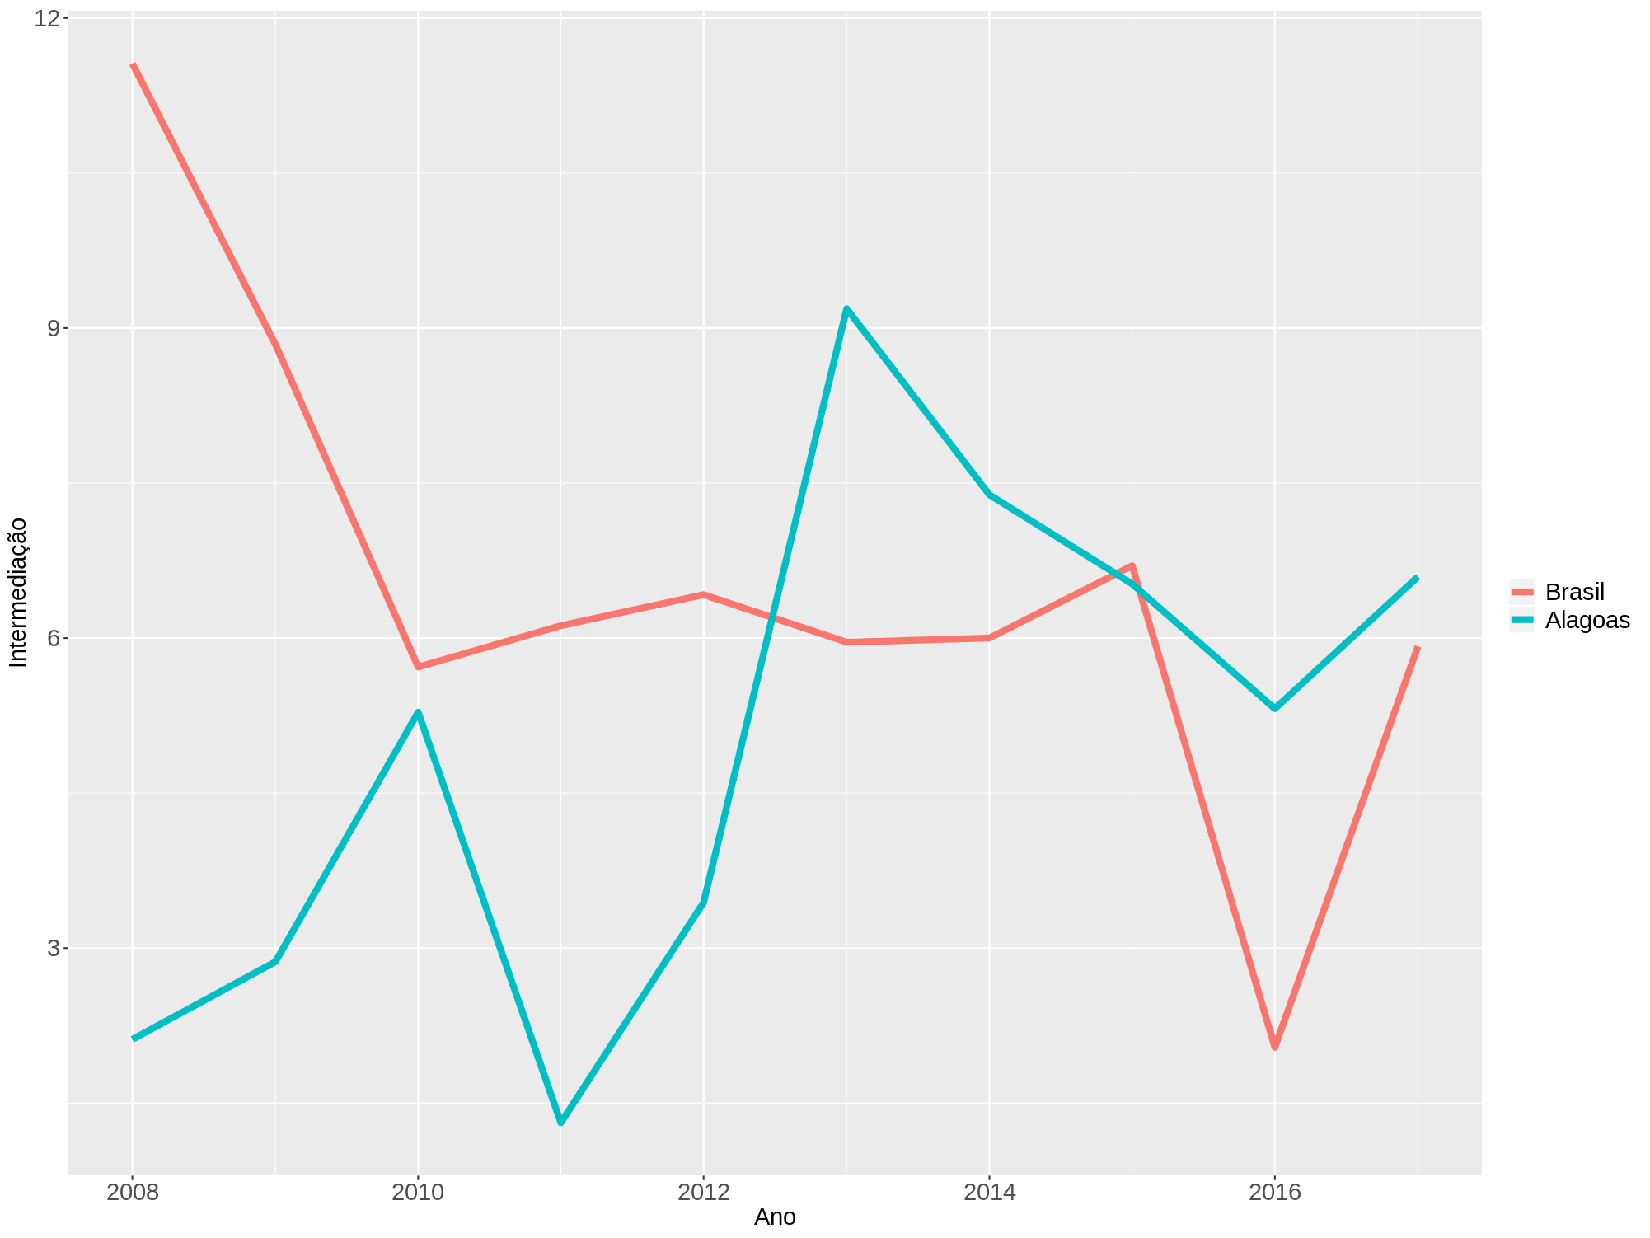
\includegraphics[scale=0.4]{Imagens/graf-linha-betweeness-br-al.pdf}
	\caption{Centralidade de Proximidade (\textit{Health Sciences})}
	\label{between-health-1}
\end{figure}

\subsubsection{Agricultural Sciences}

\begin{figure}[H]
	\centering
	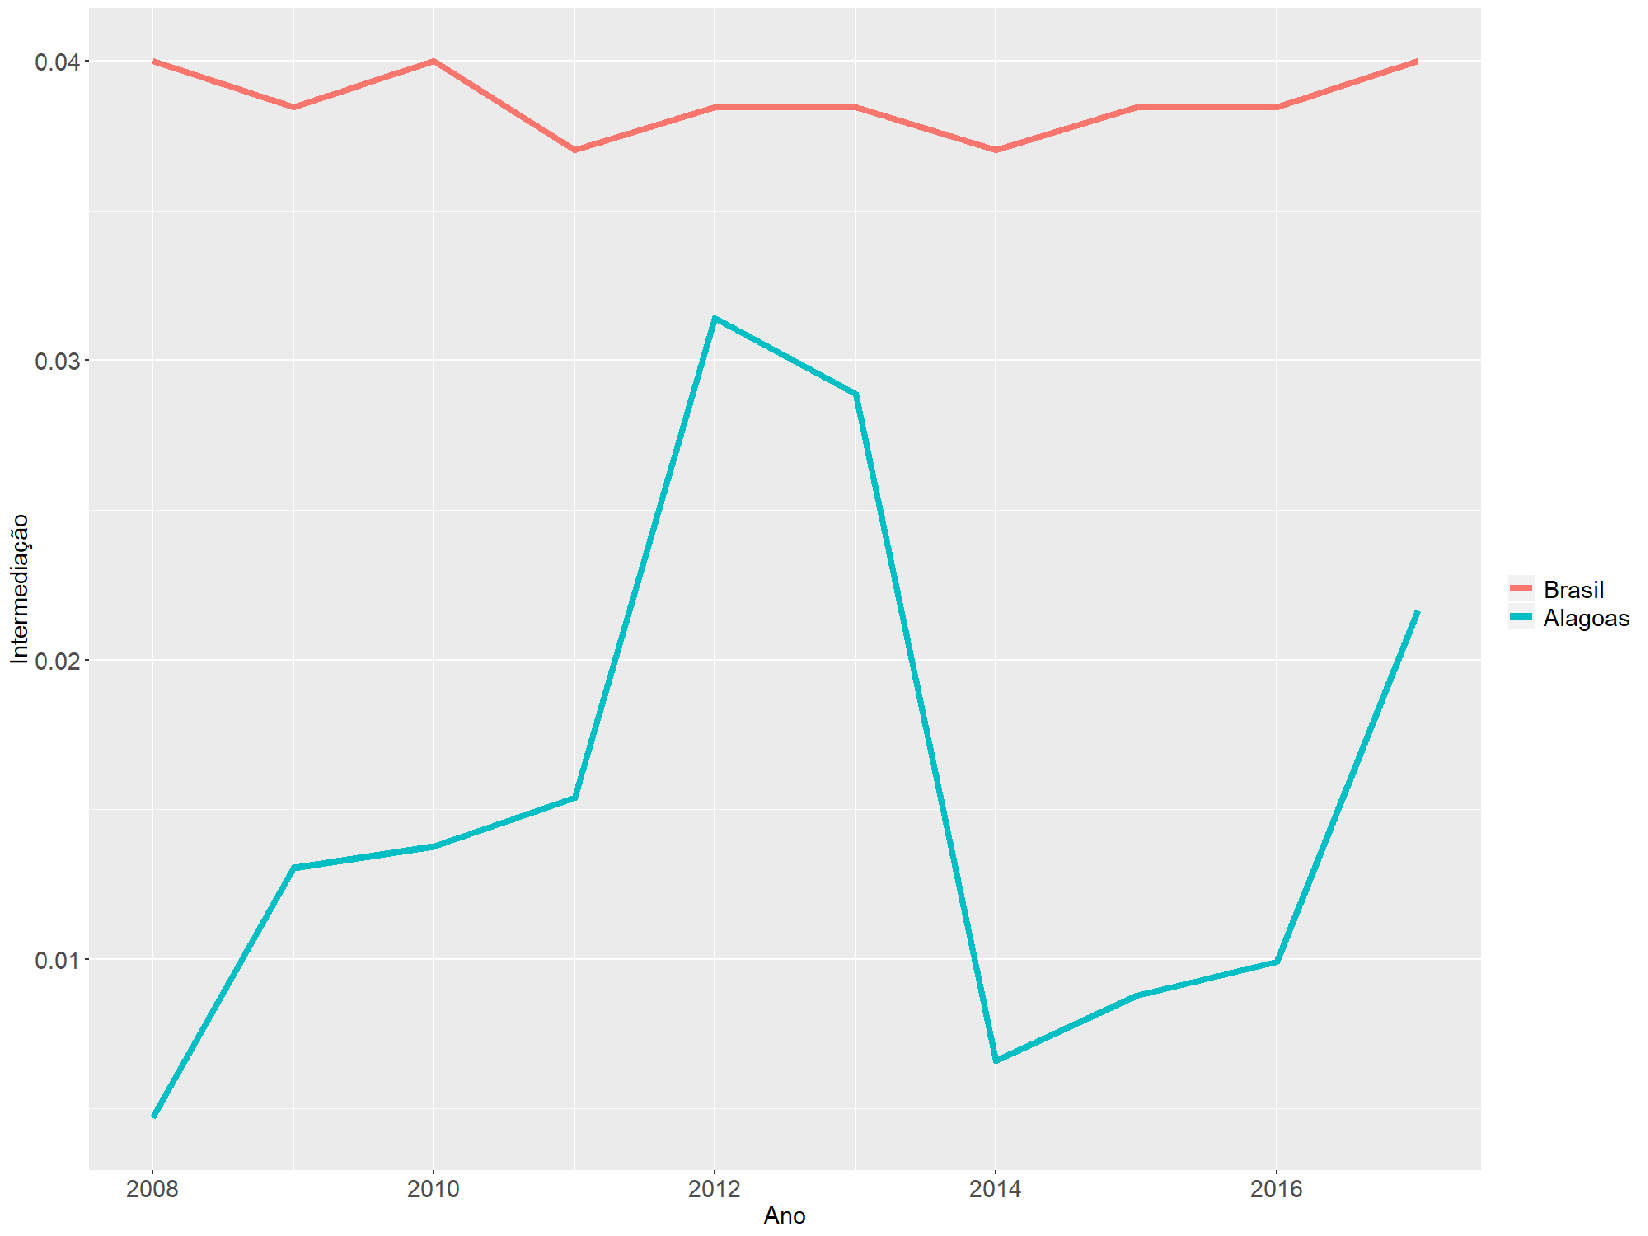
\includegraphics[scale=0.4]{Imagens/agricultural/graf-linha-betweeness-br-al.pdf}
	\caption{Centralidade de Proximidade (\textit{Agricultural Sciences})}
	\label{between-agri-1}
\end{figure}

\subsubsection{Exact and Earth Sciences}

\begin{figure}[H]
	\centering
	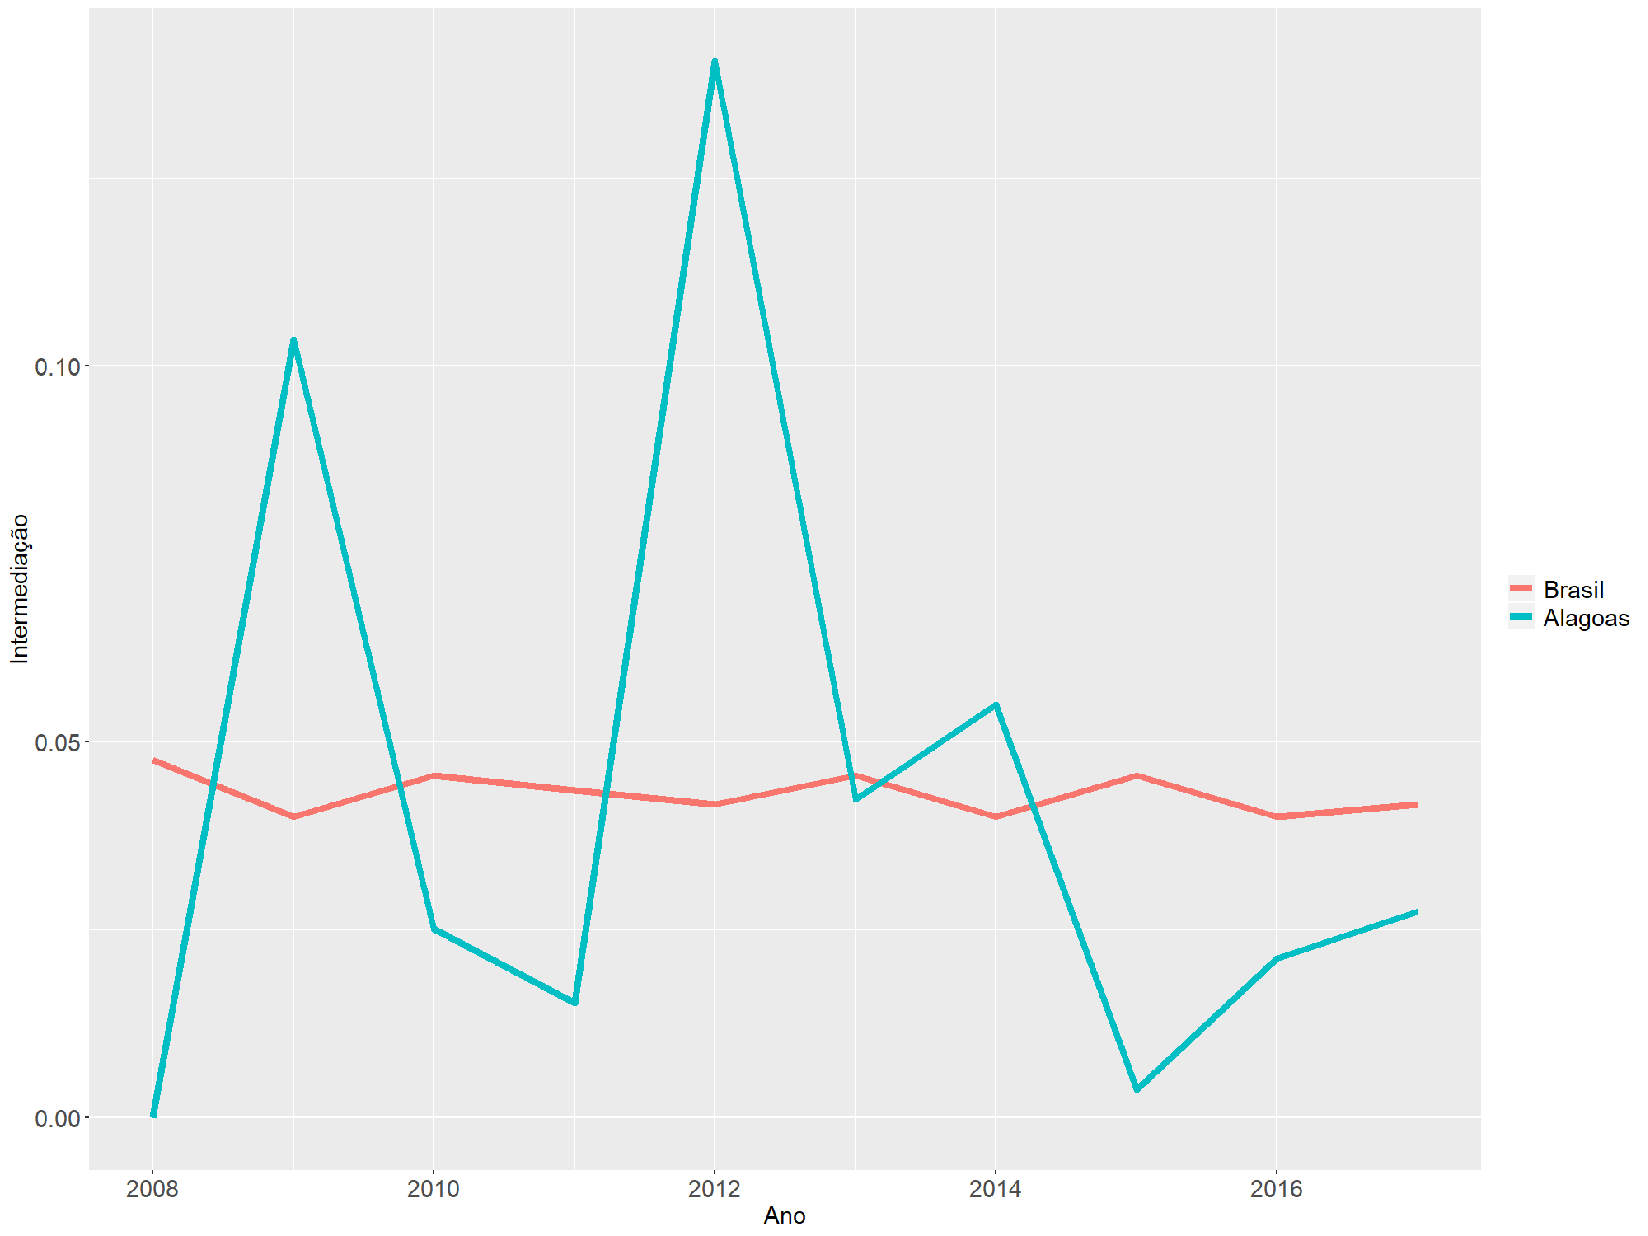
\includegraphics[scale=0.4]{Imagens/exact/graf-linha-betweeness-br-al.pdf}
	\caption{Centralidade de Proximidade (\textit{Exact and Earth Sciences})}
	\label{between-exact-1}
\end{figure}

Na observação dos gráficos da centralidade de intermediação \ref{between-health-1}, \ref{between-agri-1}, \ref{between-exact-1} verificamos que diferentemente do que se observou na centralidade do grau e de proximidade, a relação encontrada entre a Rede Brasil e Alagoas é de uma função matemática não trivial, destacando a sensibilidade dessa medida de centralidade para avaliação da colaboração científica. 


\subsubsection{Health Sciences}

\begin{figure}[H]
	\centering
	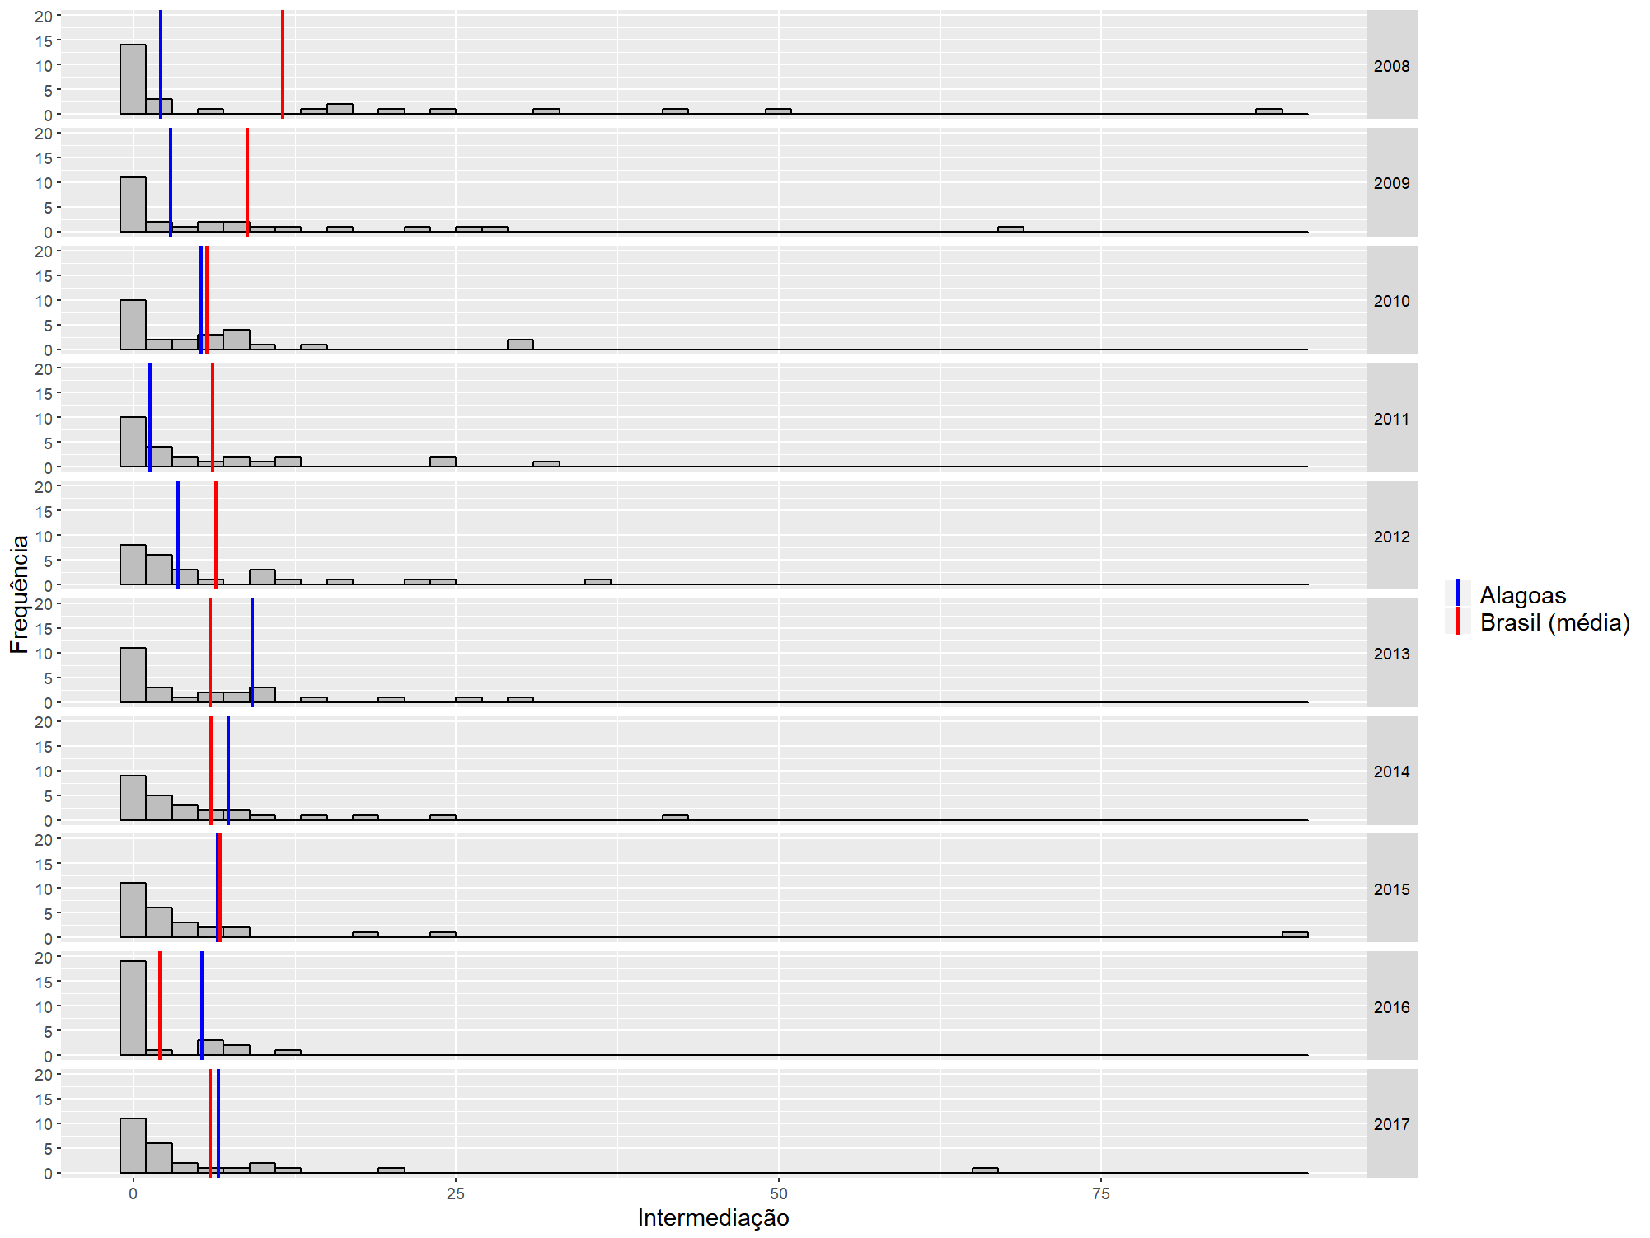
\includegraphics[scale=0.5]{Imagens/betweeness-hist.pdf}
	\caption{Histograma da Centralidade de Proximidade (\textit{Health Sciences})}
       \label{hist-health-between-1}
\end{figure}

\subsubsection{Agricultural Sciences}

\begin{figure}[H]
	\centering
	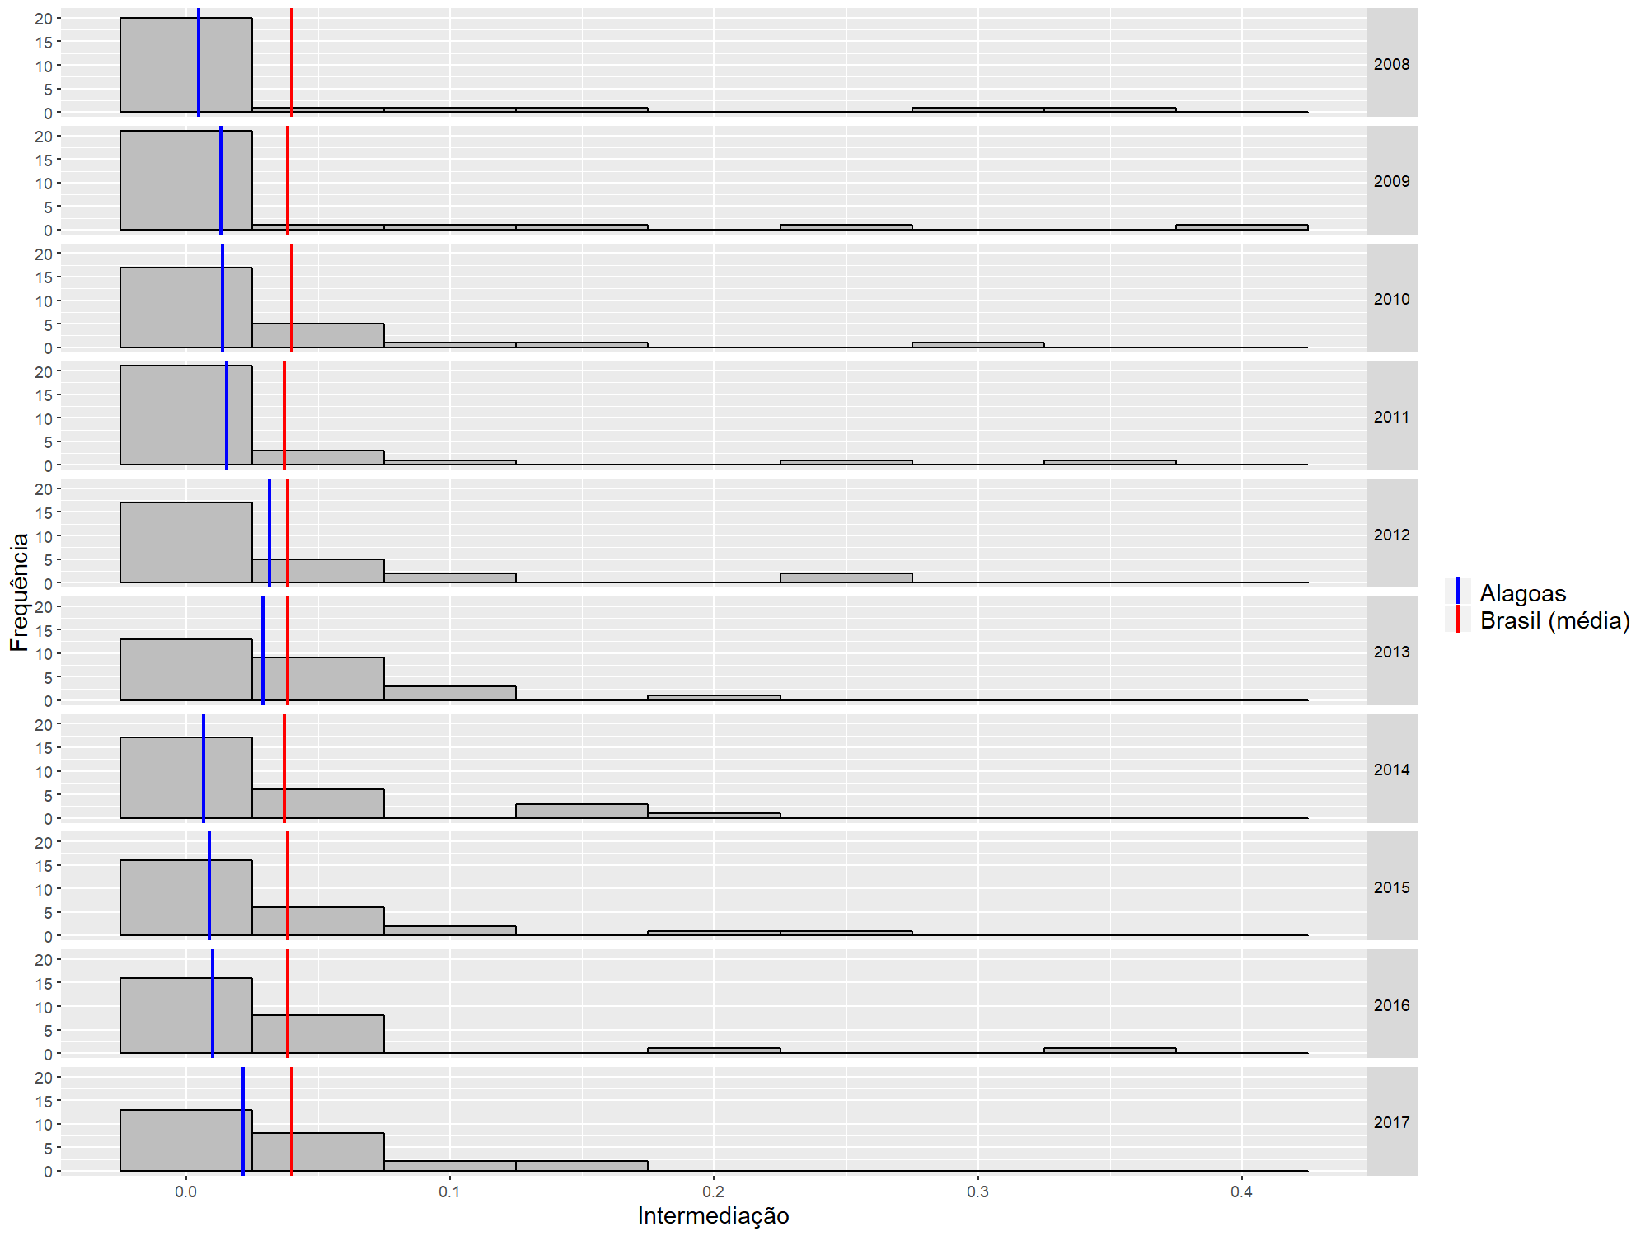
\includegraphics[scale=0.5]{Imagens/agricultural/betweeness-hist.pdf}
	\caption{Histograma da Centralidade de Proximidade (\textit{Agricultural Sciences})}
	\label{hist-agri-between-1}
\end{figure}

\subsubsection{Exact and Earth Sciences}

\begin{figure}[H]
	\centering
	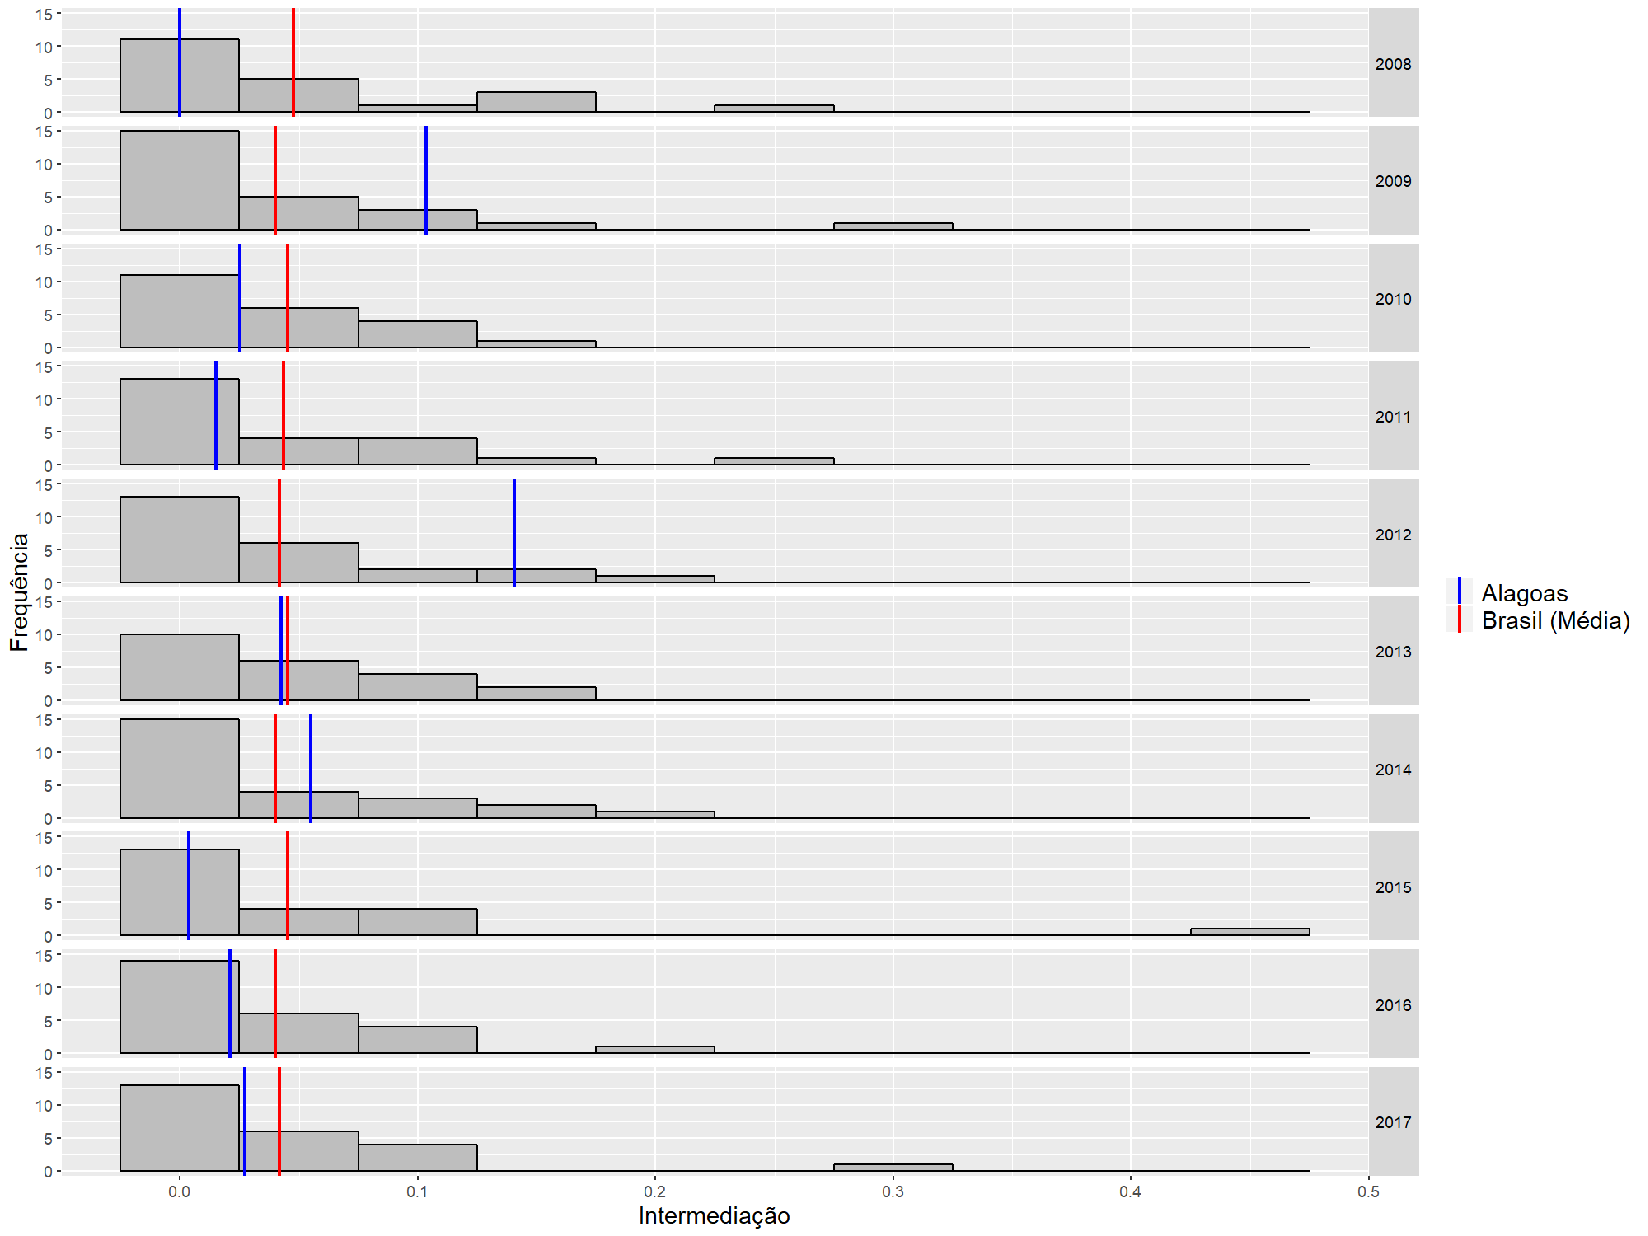
\includegraphics[scale=0.5]{Imagens/exact/betweeness-hist.pdf}
	\caption{Histograma da Centralidade de Proximidade (\textit{Exact and Earth Sciences})}
    \label{hist-exact-between-1}
\end{figure}

%%% TABELA RANKING

\section{\textbf{Ranking das Medidas de Centralidade}}

Nesta seção apresentamos os rankings por Estados (UF) em cada área do conhecimento investigadas neste trabalho. Este ranking tem por objetivo apontar o posicionamento de Alagoas frente a rede Brasil, bem como, por oportuno, mostrar os melhores e piores estados em desempenho para cada medida de centralidade da rede. Os índices foram aferidos pela média da UF em todo o período compreendido entre 2008-2017.

\subsubsection{Ranking: \textit{Health Sciences}}

\begin{table}[H]
	\centering
	\begin{tabular}{|l|l|l|l|l|l|}
		\hline
		\multicolumn{6}{|c|}{\textbf{Ranking das Medidas de Centralidade}}                                                                                                                                                        \\ \hline
		\multicolumn{2}{|c|}{\cellcolor[HTML]{C0C0C0}\textbf{Grau}} & \multicolumn{2}{c|}{\cellcolor[HTML]{C0C0C0}\textbf{Proximidade}}            & \multicolumn{2}{c|}{\cellcolor[HTML]{C0C0C0}\textbf{Intermediação}}          \\ \hline
		UF                          & Média                         & UF                                  & Média                                  & UF                                  & Média                                  \\ \hline
		SP                          & 20,50                         & SP                                  & 0,870                                  & SP                                  & 0,243                                  \\ \hline
		MG                          & 19,60                         & MG                                  & 0,839                                  & MG                                  & 0,145                                  \\ \hline
		RJ                          & 19,00                         & RJ                                  & 0,818                                  & RJ                                  & 0,093                                  \\ \hline
		RS                          & 17,60                         & RS                                  & 0,784                                  & GO                                  & 0,065                                  \\ \hline
		SC                          & 16,90                         & SC                                  & 0,770                                  & CE                                  & 0,060                                  \\ \hline
		PE                          & 16,70                         & PE                                  & 0,765                                  & SC                                  & 0,051                                  \\ \hline
		CE                          & 15,80                         & CE                                  & 0,745                                  & RS                                  & 0,049                                  \\ \hline
		RN                          & 15,20                         & RN                                  & 0,725                                  & PE                                  & 0,038                                  \\ \hline
		BA                          & 14,60                         & \textbf{AL} & \textbf{0,717} & \textbf{AL} & \textbf{0,038} \\ \hline
		\textbf{AL}                 & \textbf{14,50}                & BA                                  & 0,715                                  & RN                                  & 0,032                                  \\ \hline
		PB                          & 14,50                         & PB                                  & 0,707                                  & PR                                  & 0,030                                  \\ \hline
		PR                          & 13,80                         & PR                                  & 0,700                                  & PA                                  & 0,025                                  \\ \hline
		GO                          & 13,40                         & GO                                  & 0,690                                  & AM                                  & 0,023                                  \\ \hline
		ES                          & 12,50                         & ES                                  & 0,678                                  & PB                                  & 0,021                                  \\ \hline
		PA                          & 12,00                         & PA                                  & 0,660                                  & BA                                  & 0,016                                  \\ \hline
		SE                          & 11,40                         & SE                                  & 0,650                                  & RO                                  & 0,016                                  \\ \hline
		MT                          & 10,80                         & AM                                  & 0,641                                  & MA                                  & 0,015                                  \\ \hline
		AM                          & 10,70                         & MT                                  & 0,641                                  & MT                                  & 0,014                                  \\ \hline
		PI                          & 9,90                          & PI                                  & 0,616                                  & ES                                  & 0,012                                  \\ \hline
		MA                          & 9,40                          & MA                                  & 0,614                                  & PI                                  & 0,004                                  \\ \hline
		MS                          & 5,30                          & AP                                  & 0,557                                  & SE                                  & 0,004                                  \\ \hline
		AC                          & 4,90                          & RO                                  & 0,552                                  & AC                                  & 0,001                                  \\ \hline
		RO                          & 4,22                          & MS                                  & 0,538                                  & MS                                  & 0,001                                  \\ \hline
		RR                          & 3,70                          & AC                                  & 0,518                                  & AP                                  & 0,000                                  \\ \hline
		AP                          & 3,63                          & RR                                  & 0,500                                  & DF                                  & 0,000                                  \\ \hline
		TO                          & 2,33                          & TO                                  & 0,495                                  & RR                                  & 0,000                                  \\ \hline
		DF                          & 1,00                          & DF                                  & 0,436                                  & TO                                  & 0,000                                  \\ \hline
	\end{tabular}
	\caption{Ranking Medidas de Centralidade (\textit{Health Sciences})}
	\label{rank-health}
\end{table}

\subsubsection{Ranking: \textit{Agricultural Sciences}}

\begin{table}[H]
	\centering
	\begin{tabular}{|l|l|l|l|l|l|}
		\hline
		\multicolumn{6}{|c|}{\textbf{Ranking das Medidas de Centralidade}}                                                                                                                                    \\ \hline
		\multicolumn{2}{|c|}{\cellcolor[HTML]{C0C0C0}\textbf{Grau}} & \multicolumn{2}{c|}{\cellcolor[HTML]{C0C0C0}\textbf{Proximidade}} & \multicolumn{2}{c|}{\cellcolor[HTML]{C0C0C0}\textbf{Intermediação}} \\ \hline
		UF                          & Média                         & UF                     & Média                                    & UF                              & Média                             \\ \hline
		RN                          & 24,10                         & MG                     & 0,889                                    & MG                              & 0,213                             \\ \hline
		MG                          & 23,20                         & RN                     & 0,877                                    & RN                              & 0,205                             \\ \hline
		PE                          & 17,60                         & RS                     & 0,786                                    & RS                              & 0,115                             \\ \hline
		RS                          & 17,20                         & PE                     & 0,740                                    & PB                              & 0,067                             \\ \hline
		PB                          & 16,60                         & PB                     & 0,718                                    & GO                              & 0,067                             \\ \hline
		RJ                          & 15,80                         & RJ                     & 0,701                                    & PE                              & 0,062                             \\ \hline
		MT                          & 14,40                         & MT                     & 0,675                                    & RJ                              & 0,042                             \\ \hline
		GO                          & 14,10                         & GO                     & 0,665                                    & CE                              & 0,031                             \\ \hline
		CE                          & 13,30                         & CE                     & 0,652            & MT      & 0,031     \\ \hline
		PA                          & 13,30                         & PA                     & 0,651                                    & PA                              & 0,020                             \\ \hline
		PR                          & 12,70                         & BA                     & 0,636                                    & PR                              & 0,020                             \\ \hline
		BA                          & 12,60                         & PR                     & 0,635                                    & MS                              & 0,018                             \\ \hline
		\textbf{AL}                 & \textbf{12,00}                & \textbf{AL}            & \textbf{0,625}                           & PI                              & 0,017                             \\ \hline
		PI                          & 11,80                         & ES                     & 0,625                                    & ES                              & 0,016                             \\ \hline
		ES                          & 11,70                         & PI                     & 0,624                                    & BA                              & 0,016                             \\ \hline
		MS                          & 10,90                         & MS                     & 0,609                                    & \textbf{AL}                     & \textbf{0,015}                    \\ \hline
		SC                          & 9,70                          & TO                     & 0,589                                    & SC                              & 0,009                             \\ \hline
		TO                          & 9,50                          & SP                     & 0,580                                    & SP                              & 0,008                             \\ \hline
		SP                          & 9,20                          & SC                     & 0,576                                    & AC                              & 0,008                             \\ \hline
		SE                          & 8,60                          & SE                     & 0,571                                    & TO                              & 0,008                             \\ \hline
		AM                          & 7,30                          & AC                     & 0,558                                    & AM                              & 0,004                             \\ \hline
		AC                          & 7,00                          & AM                     & 0,544                                    & SE                              & 0,004                             \\ \hline
		MA                          & 7,00                          & RO                     & 0,540                                    & RO                              & 0,003                             \\ \hline
		RO                          & 6,22                          & MA                     & 0,537                                    & MA                              & 0,002                             \\ \hline
		RR                          & 5,50                          & RR                     & 0,526                                    & RR                              & 0,000                             \\ \hline
		DF                          & 2,40                          & AP                     & 0,490                                    & AP                              & 0,000                             \\ \hline
		AP                          & 2,20                          & DF                     & 0,423                                    & DF                              & 0,000                             \\ \hline
	\end{tabular}
	\caption{Ranking Medidas de Centralidade (\textit{Agricultural Sciences})}
	\label{rank-agri}
\end{table}


\subsubsection{Ranking: \textit{Exact and Earth Sciences}}

\begin{table}[H]
	\centering
	\begin{tabular}{|l|l|l|l|l|l|}
		\hline
		\multicolumn{6}{|c|}{\textbf{Ranking das Medidas de Centralidade}}                                                                                                                                             \\ \hline
		\multicolumn{2}{|c|}{\cellcolor[HTML]{C0C0C0}\textbf{Grau}} & \multicolumn{2}{c|}{\cellcolor[HTML]{C0C0C0}\textbf{Proximidade}} & \multicolumn{2}{c|}{\cellcolor[HTML]{C0C0C0}\textbf{Intermediação}}          \\ \hline
		UF                          & Média                         & UF                     & Média                                    & UF                                  & Média                                  \\ \hline
		RJ                          & 13,40                         & MG                     & 0,657                                    & MG                                  & 0,173                                  \\ \hline
		MG                          & 13,30                         & RJ                     & 0,651                                    & RJ                                  & 0,144                                  \\ \hline
		SP                          & 11,40                         & SP                     & 0,618                                    & SP                                  & 0,091                                  \\ \hline
		RS                          & 10,60                         & RS                     & 0,601                                    & RS                                  & 0,071                                  \\ \hline
		PB                          & 9,80                          & RN                     & 0,581                                    & RN                                  & 0,059                                  \\ \hline
		RN                          & 9,70                          & PB                     & 0,566                                    & PE                                  & 0,055                                  \\ \hline
		PE                          & 9,50                          & PE                     & 0,565                                    & PB                                  & 0,054                                  \\ \hline
		PR                          & 9,10                          & BA                     & 0,559                                    & PR                                  & 0,049                                  \\ \hline
		BA                          & 8,70                          & SC                     & 0,556            & \textbf{AL} & \textbf{0,043} \\ \hline
		SC                          & 8,50                          & PR                     & 0,555                                    & CE                                  & 0,043                                  \\ \hline
		CE                          & 8,20                          & CE                     & 0,554                                    & SC                                  & 0,039                                  \\ \hline
		\textbf{AL}                 & \textbf{7,90}                 & \textbf{AL}            & \textbf{0,528}                           & PI                                  & 0,036                                  \\ \hline
		PA                          & 6,20                          & GO                     & 0,512                                    & BA                                  & 0,029                                  \\ \hline
		SE                          & 6,10                          & ES                     & 0,485                                    & GO                                  & 0,029                                  \\ \hline
		GO                          & 6,00                          & SE                     & 0,483                                    & PA                                  & 0,025                                  \\ \hline
		AM                          & 5,60                          & AM                     & 0,480                                    & SE                                  & 0,018                                  \\ \hline
		ES                          & 5,60                          & PA                     & 0,473                                    & MT                                  & 0,013                                  \\ \hline
		PI                          & 5,10                          & PI                     & 0,472                                    & AM                                  & 0,012                                  \\ \hline
		MT                          & 4,67                          & RO                     & 0,442                                    & MA                                  & 0,010                                  \\ \hline
		MS                          & 3,63                          & MT                     & 0,435                                    & ES                                  & 0,006                                  \\ \hline
		MA                          & 3,50                          & MS                     & 0,412                                    & RO                                  & 0,002                                  \\ \hline
		RO                          & 3,25                          & TO                     & 0,411                                    & MS                                  & 0,001                                  \\ \hline
		RR                          & 2,40                          & MA                     & 0,404                                    & AC                                  & 0,000                                  \\ \hline
		TO                          & 2,17                          & RR                     & 0,395                                    & AP                                  & 0,000                                  \\ \hline
		DF                          & 2,00                          & AP                     & 0,388                                    & DF                                  & 0,000                                  \\ \hline
		AP                          & 2,00                          & AC                     & 0,384                                    & RR                                  & 0,000                                  \\ \hline
		AC                          & 1,80                          & DF                     & 0,000                                    & TO                                  & 0,000                                  \\ \hline
	\end{tabular}
	\caption{Ranking Medidas de Centralidade (\textit{Exact and Earth Sciences})}
	\label{rank-exact}
\end{table}


\section{\textbf{Discussão dos Resultados}}

Esta seção tem a por objetivo a discussão dos resultados obtidos neste trabalho, os estudo de redes de coautorias por medidas de centralidade de redes complexas, e a contextualização destes ao comportamento da colaboração científica. A metodologia aplicada permitiu a compreensão das características estruturais das redes, e a determinação destas para os estudos exploratórios.

Utilizando o vértice focal Alagoas, podemos comparar nas três áreas do conhecimento selecionadas para esse trabalho, o estudo das três medidas de centralidade, elencadas por \citep{freeman1991centrality} como essenciais ao estudo de redes.

Numérica e graficamente percebemos que para todas as áreas o comportamento a medida da centralidade de grau e de proximidade para o vértice amostral utilizado e a média parâmetro de estudo, em que estas possuem relações de correlações, quer seja positiva ou negativa, forte ou fraca para cada período (ano) em análise; o que não se observa para a centralidade de intermediação que em todas as áreas apresentou resultados \textit{sui generis} indicando assim, uma sensibilidade desta medida.

%Dentro dos conceitos e propriedades das medidas de centralidade de redes, criamos a seguinte contextualização para a melhor interpretação em redes de coautoria.

%\begin{itemize}
%	\item \textbf{Centralidade do Grau:} \\
%	“Um nó importante está conectado com muitos nós.” \\
%	"Um coautor importante está conectado a muitos coautores.”
	
%	\item \textbf{Centralidade de Proximidade:} \\
%	“Um nó importante faz parte de muitos caminhos". \\
%	"Um coautor importante faz parte de muitos caminhos.” 	
	
%	\item \textbf{Centralidade de Intermediação:} \\
%	“Um nó importante está próximo dos outros nós.” \\
%	"Um coautor importante está próximo dos outros coautores.”
	
%\end{itemize}

As medidas de centralidade utilizadas neste trabalhou permitiu a construção de rankings por área, indicando assim os índices aferidos pelos estados para o período de 2008-2017, possibilitando o conhecimento da colaboração científica a partir desses indicadores na base de dados e nas áreas estudadas.

Na área de \textit{Health Sciences} verificamos que conforme o ranking na figura \ref{rank-health} os estados em destaque são: São Paulo, Minas Gerais e Rio de Janeiro são os estados que possuem os maiores índices das medidas de centralidade: de grau, de proximidade, de intermediação. Alagoas assume a décima posição junto com Pernambuco para a centralidade do grau. E a nona posição para centralidade de proximidade e de intermediação, nesta última em empate também com Pernambuco.

Em \textit{Agricultural Sciences} o destaque é para os estados do Rio Grande do Norte, Minas Gerais e Rio Grande do Sul (conforme ranking \ref{rank-agri}); tendo Alagoas assumido respectivamente as posições de décimo terceiro para centralidade do grau e de proximidade; décimo sexto para intermediação. 

Salientamos que outros estudos exploratórios podem realizar detalhamentos a respeito de comunidades e cliques existentes na rede, a fim de encontrar padrões de relacionamentos interinstitucionais. 

Neste trabalho, a análise proposta traz à tona um conhecimento até então desconhecido, a avaliação da colaboração científica pelas redes de coautoria no período de 2008 à 2017, base SciELO das áreas estudadas. E que as medidas com suas respectivas propriedades podem subsidiar estudos investigativos e exploratórios para a avaliação de outras redes, e fatores que possam influenciar o comportamento delas.

\mychapter{\textsc{Conclusões}}{chp:conclusoes}
\lhead{\textsc{Conclusões}}

\lettrine{A} seguir apresentamos nossas considerações finais, buscando a contextualização do problema de pesquisa em tela com os resultados obtidos e as sugestões para trabalhos futuros.

\section{\textbf{Considerações Finais}} 

Com a proposta apresentada, buscamos destacar a importância do estudo de redes de coautorias relacionando ao arcabouço teórico de redes complexas e a relação com a colaboração científica, neste trabalho a compreensão da interação existente entre as Universidades Federais do Brasil e a Universidade Federal de Alagoas.

Conforme \citep{Barabasi2001}, os estudos de redes de coautoria são importantes e possuem sua relevância para apresentar padrões de comportamento e possibilitar modelos preditivos de quais áreas ou campos estão se desenvolvendo, são emergentes, ou quais tendências possuem.

O estudo das redes de coautoria deste trabalho, mostrou um resultado que se aplicado a outras redes poderão descrever o comportamento, dinâmica e características, quando se observa as relações existentes dentro das áreas de \textit{Health Sciences, Agricultural Sciences e Exact and Earth Sciences}, a partir da consideração de uma base de indexação de artigos específica ou de outra.

As medidas de centralidade possibilitam aferir conhecimento a respeito da dinâmica e do comportamento das redes de coautorias no aspecto temporal. A aplicação destas, em outras áreas do conhecimento e em outras bases de indexação de artigos científicos, mostram-se significativas para a obtenção de resultados específico para avaliação da colaboração científica, possibilitando a compreensão e caracterização dos atores de relevância e de influência da rede.


\section{\textbf{Trabalhos futuros}}

Por trabalhos futuros, consideramos a expansão do uso de outras medidas de centralidade de rede para análises topológica da interação dos vértices e arestas nas redes de coautoria. Sugerimos outras abordagens de uma prisma analítico e probabilístico, como a utilização de técnicas de \textit{network-driven approaches}, de \textit{link prediction}, análises de comunidades de influências na rede, e simulação do comportamento da rede com base em métricas de redes complexas.



 

%Apêndices e Anexos
\appendix
\chapter{\textsc{Redes de Coautoria}}~\label{redes}
\lhead{\textsc{Redes}}

As características propostas na plotagem da rede é, formato em círculo para fins comparativos, disposição dos vértices com coloração das UF pertencentes a mesma região geográfica, espessura e coloração das arestas indicando o maior volume/peso das coautorias existente entre as UFs, espessuras dos laços, indicando peso das coautorias existentes na mesma UF.

A seguir são apresentadas as redes de coautoria utilizando o vértice focal Alagoas, e então observando as conexões realizadas com os demais vértices da rede (UF). Visualmente é possível notar o crescimento pelo número de novas conexões.


%%% ÁREA HEALTH SCIENCES

\section{\textbf{Health Sciences}}

\subsubsection{Redes de Coautoria Universidades Federal do Brasil - Área: \textit{Health Sciences}}


\begin{figure}[H]
	\centering
	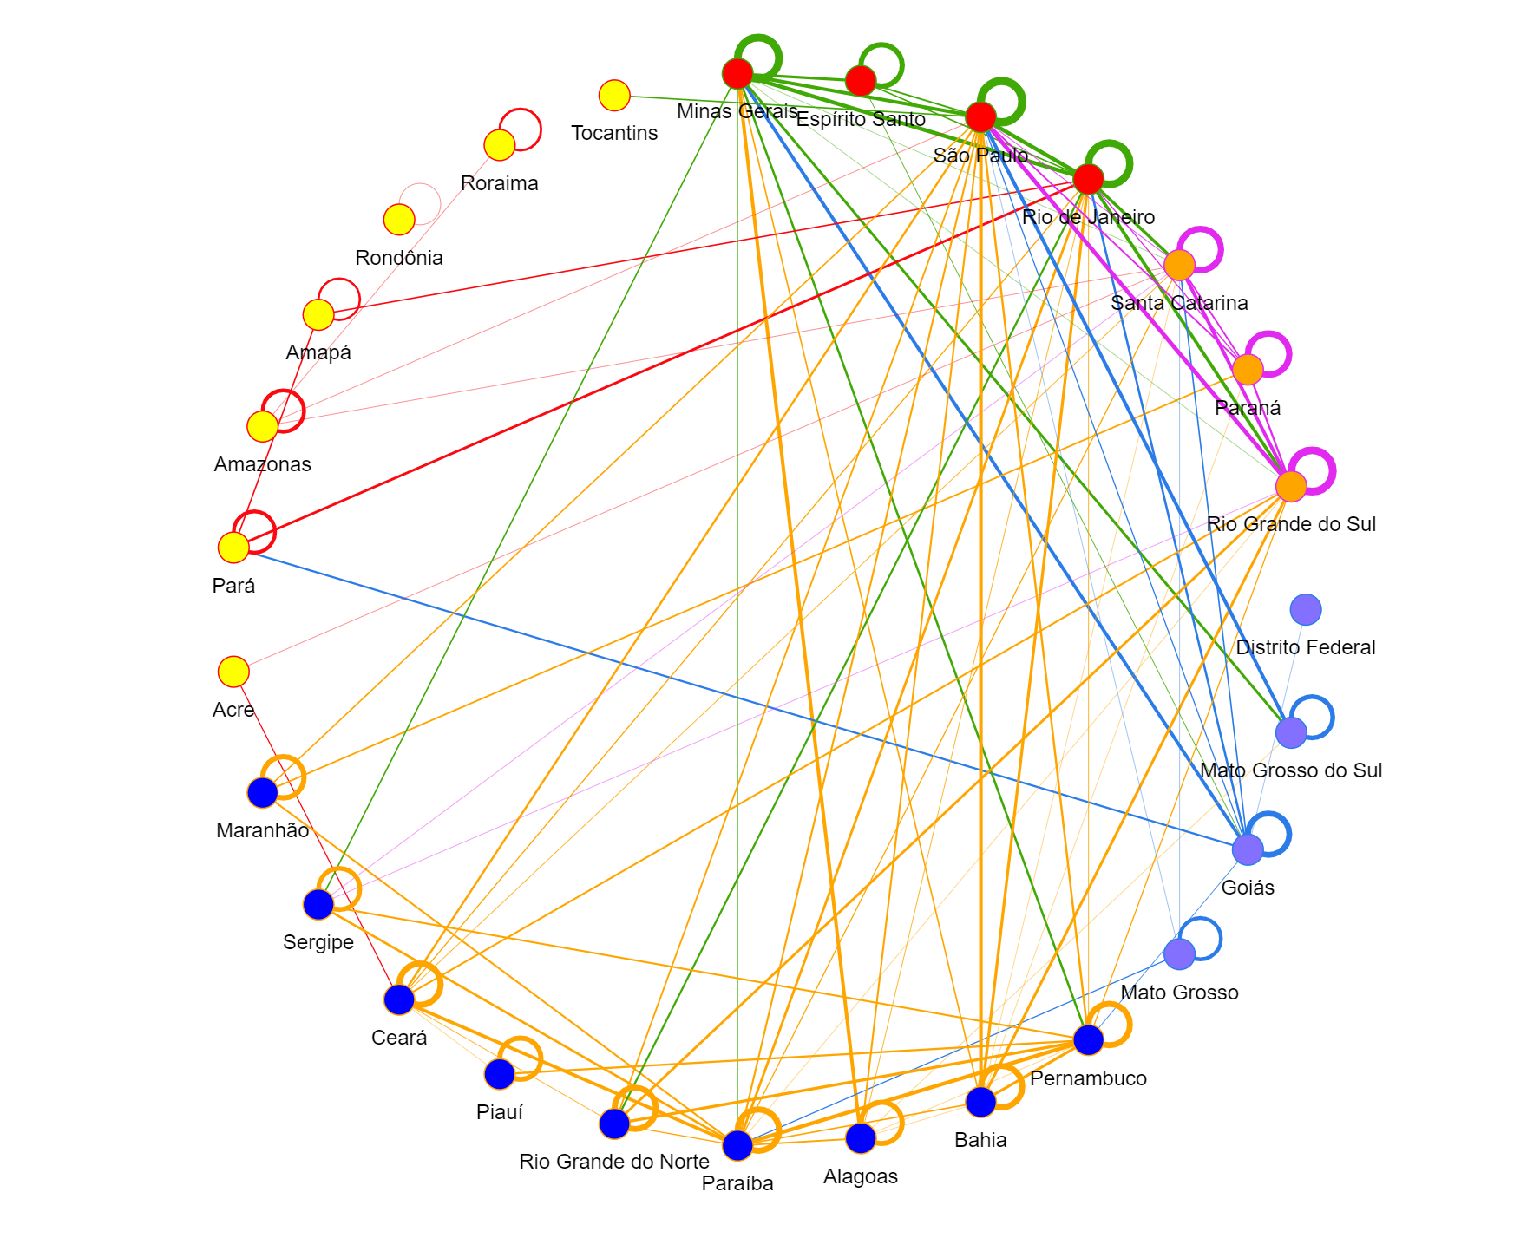
\includegraphics[scale=0.6]{Imagens/rede-2008.pdf}
	\caption{Rede de Coautoria das Universidades Federais do Brasil (\textit{Health Sciences})- 2008}
	\label{Rede de Coautoria - UF BR 2008}
\end{figure}

\begin{figure}[H]
	\centering
	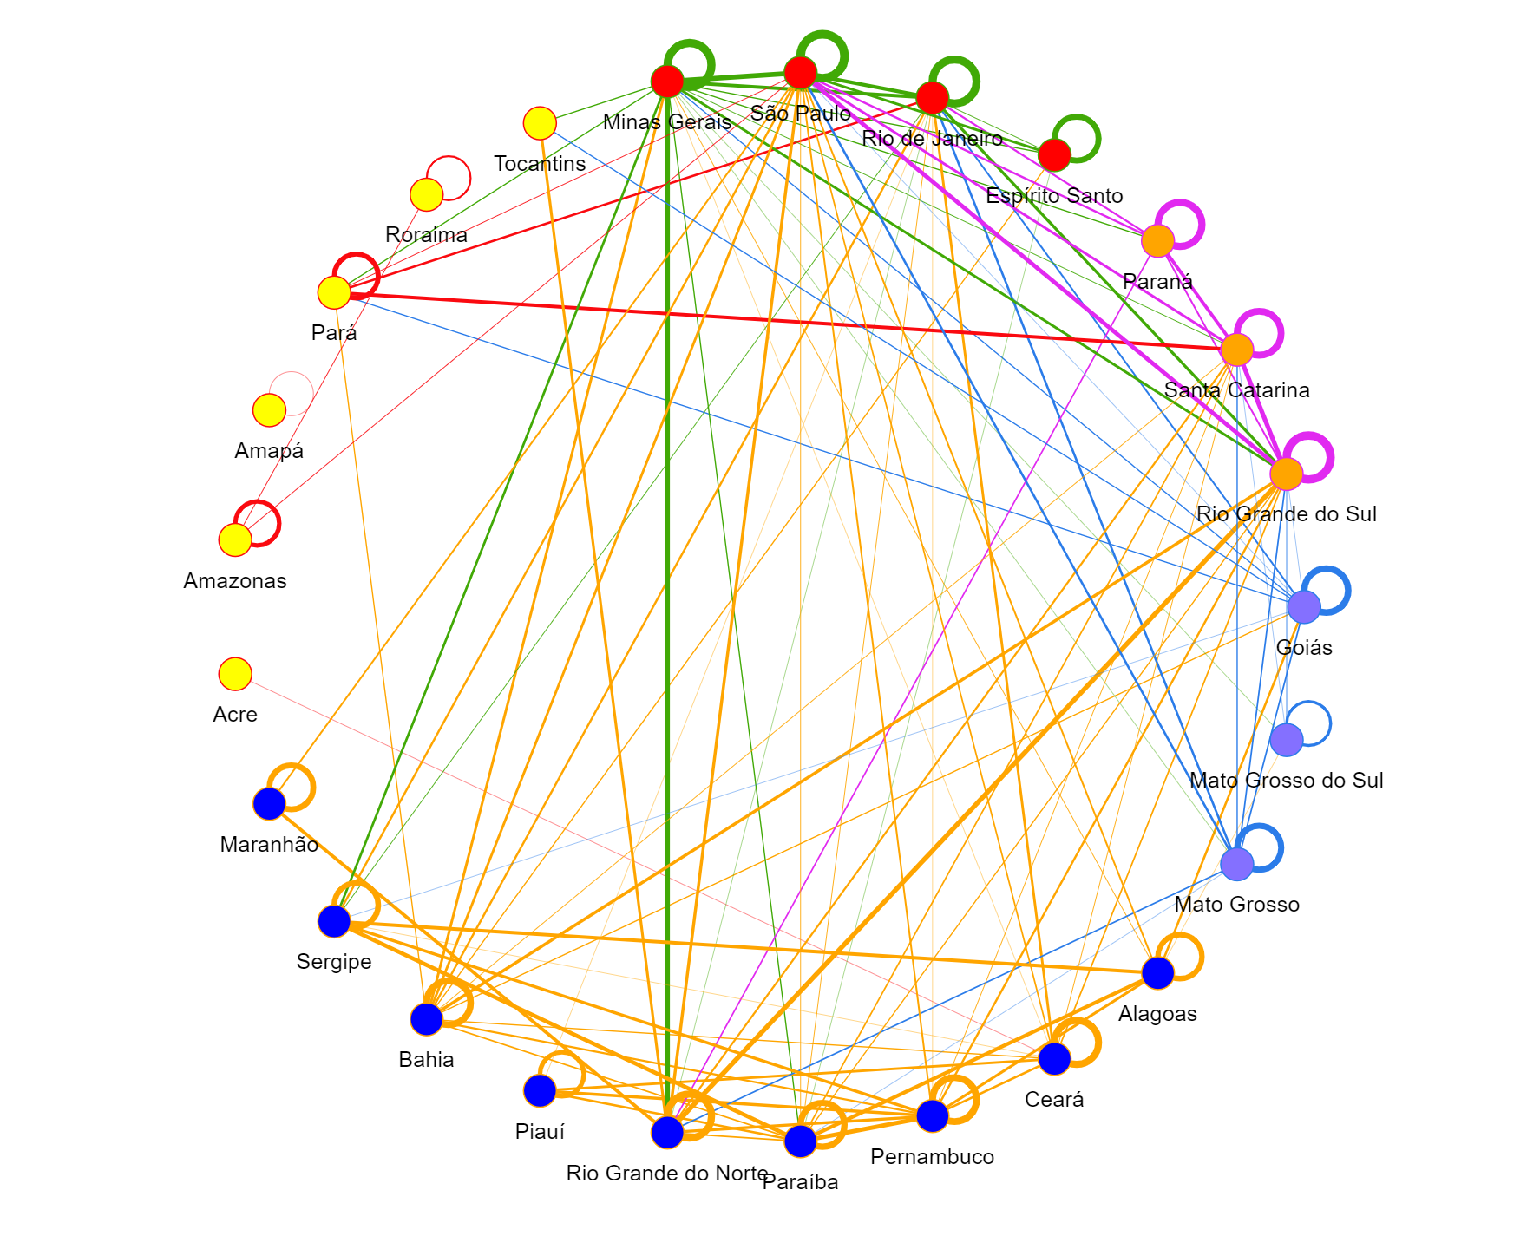
\includegraphics[scale=0.6]{Imagens/rede-2009.pdf}
	\caption{Rede de Coautoria das Universidades Federais do Brasil (\textit{Health Sciences}) - 2009}
	\label{Rede de Coautoria - UF BR 2009}
\end{figure}

\begin{figure}[H]
	\centering
	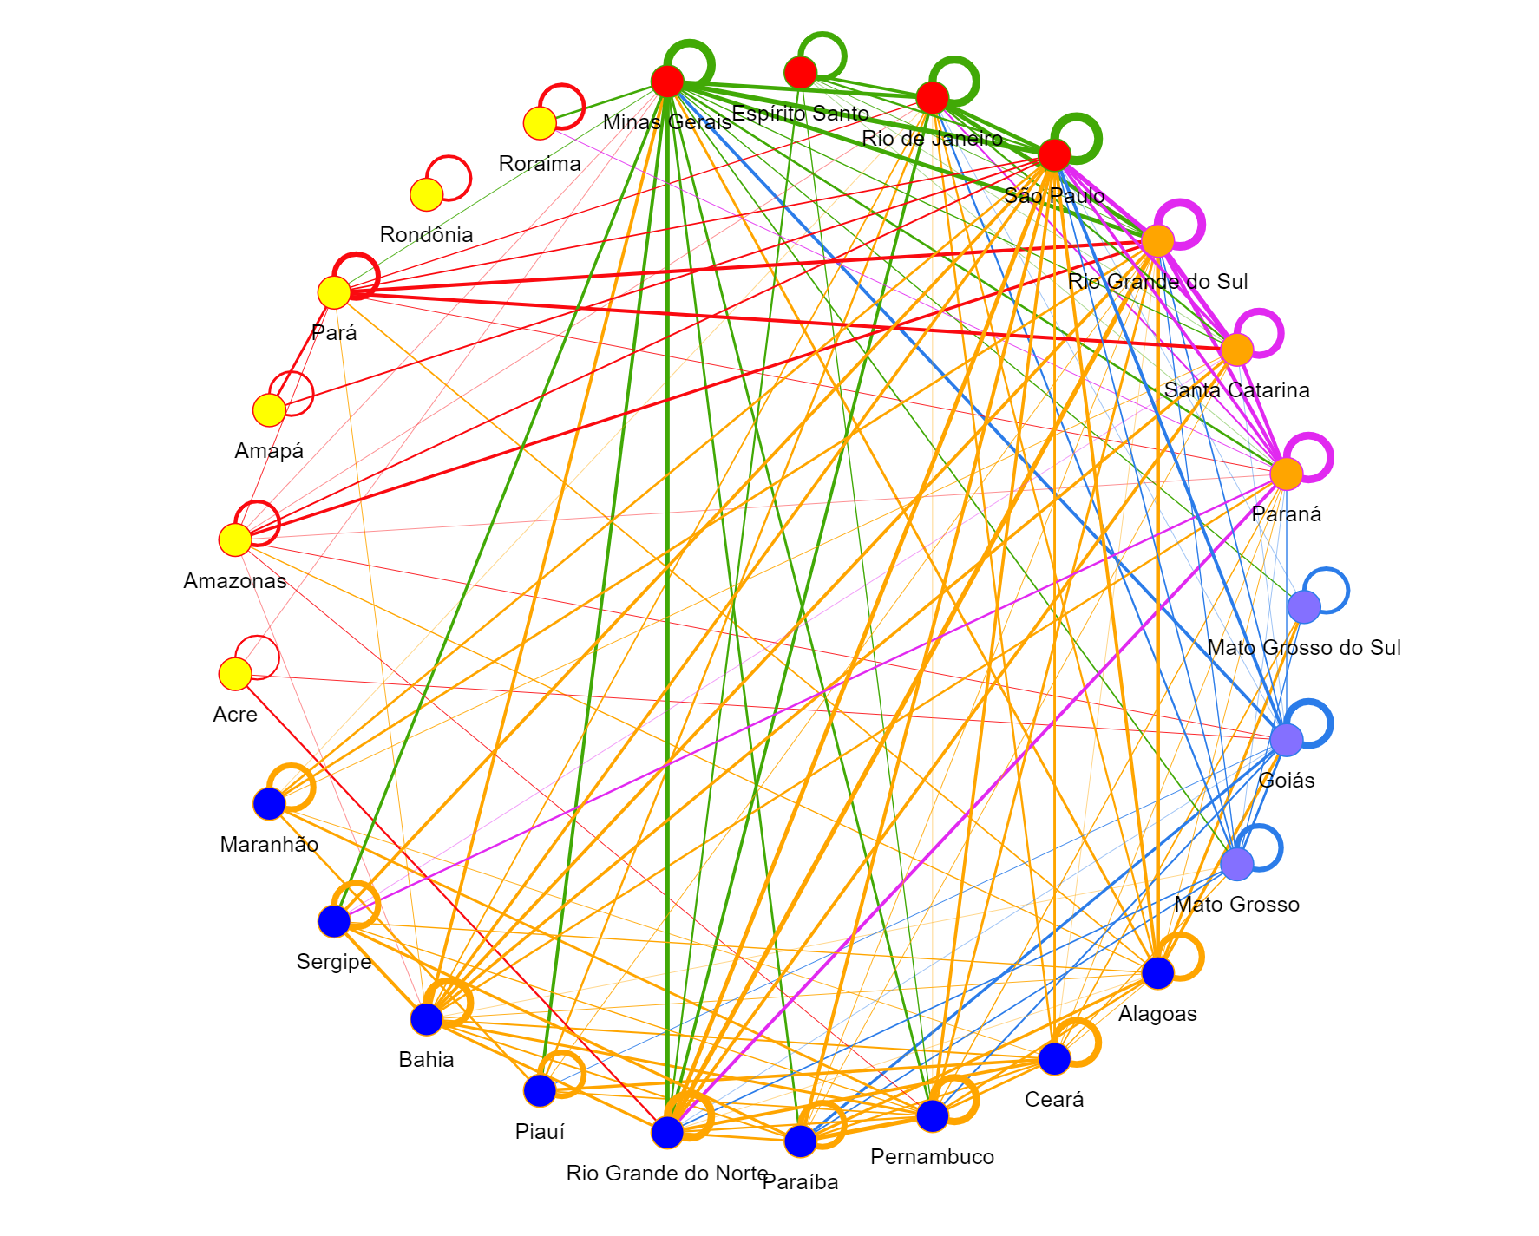
\includegraphics[scale=0.6]{Imagens/rede-2010.pdf}
	\caption{Rede de Coautoria das Universidades Federais do Brasil (\textit{Health Sciences}) - 2010}
	\label{Rede de Coautoria - UF BR 2010}
\end{figure}

\begin{figure}[H]
	\centering
	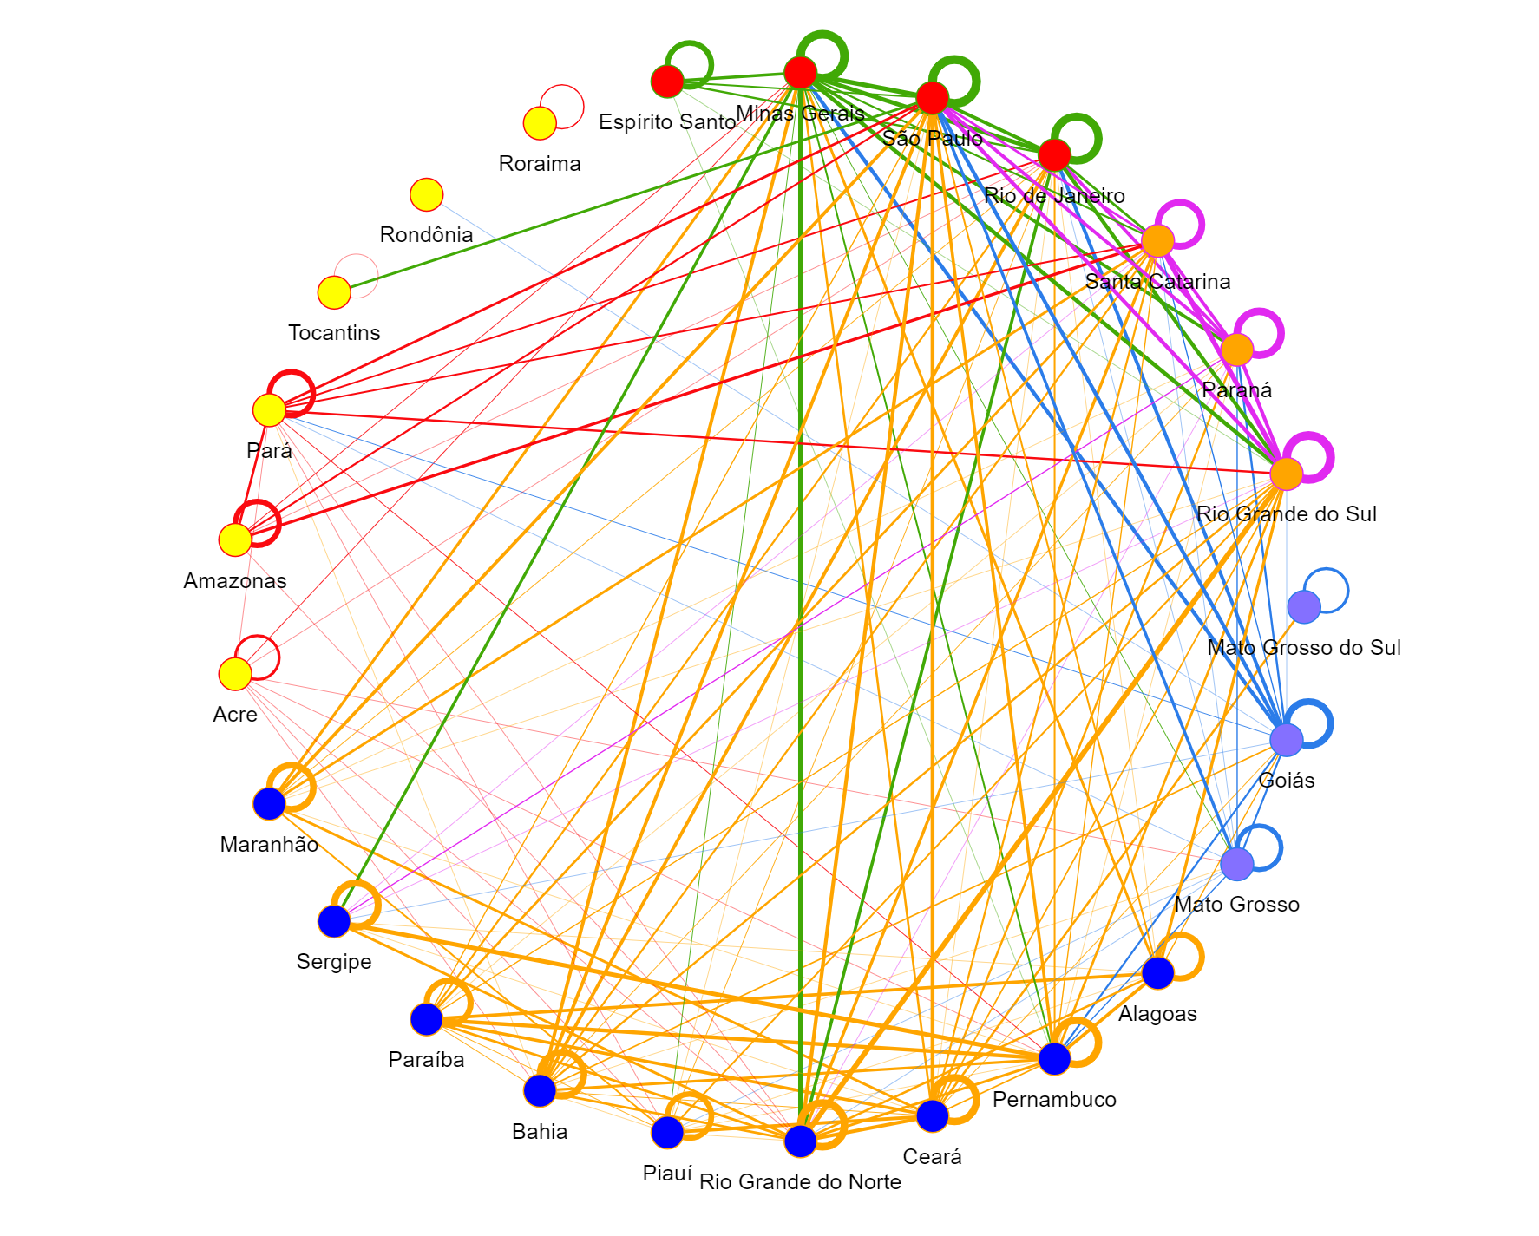
\includegraphics[scale=0.6]{Imagens/rede-2011.pdf}
	\caption{Rede de Coautoria das Universidades Federais do Brasil (\textit{Health Sciences}) - 2011}
	\label{Rede de Coautoria - UF BR 2011}
\end{figure}


\begin{figure}[H]
	\centering
	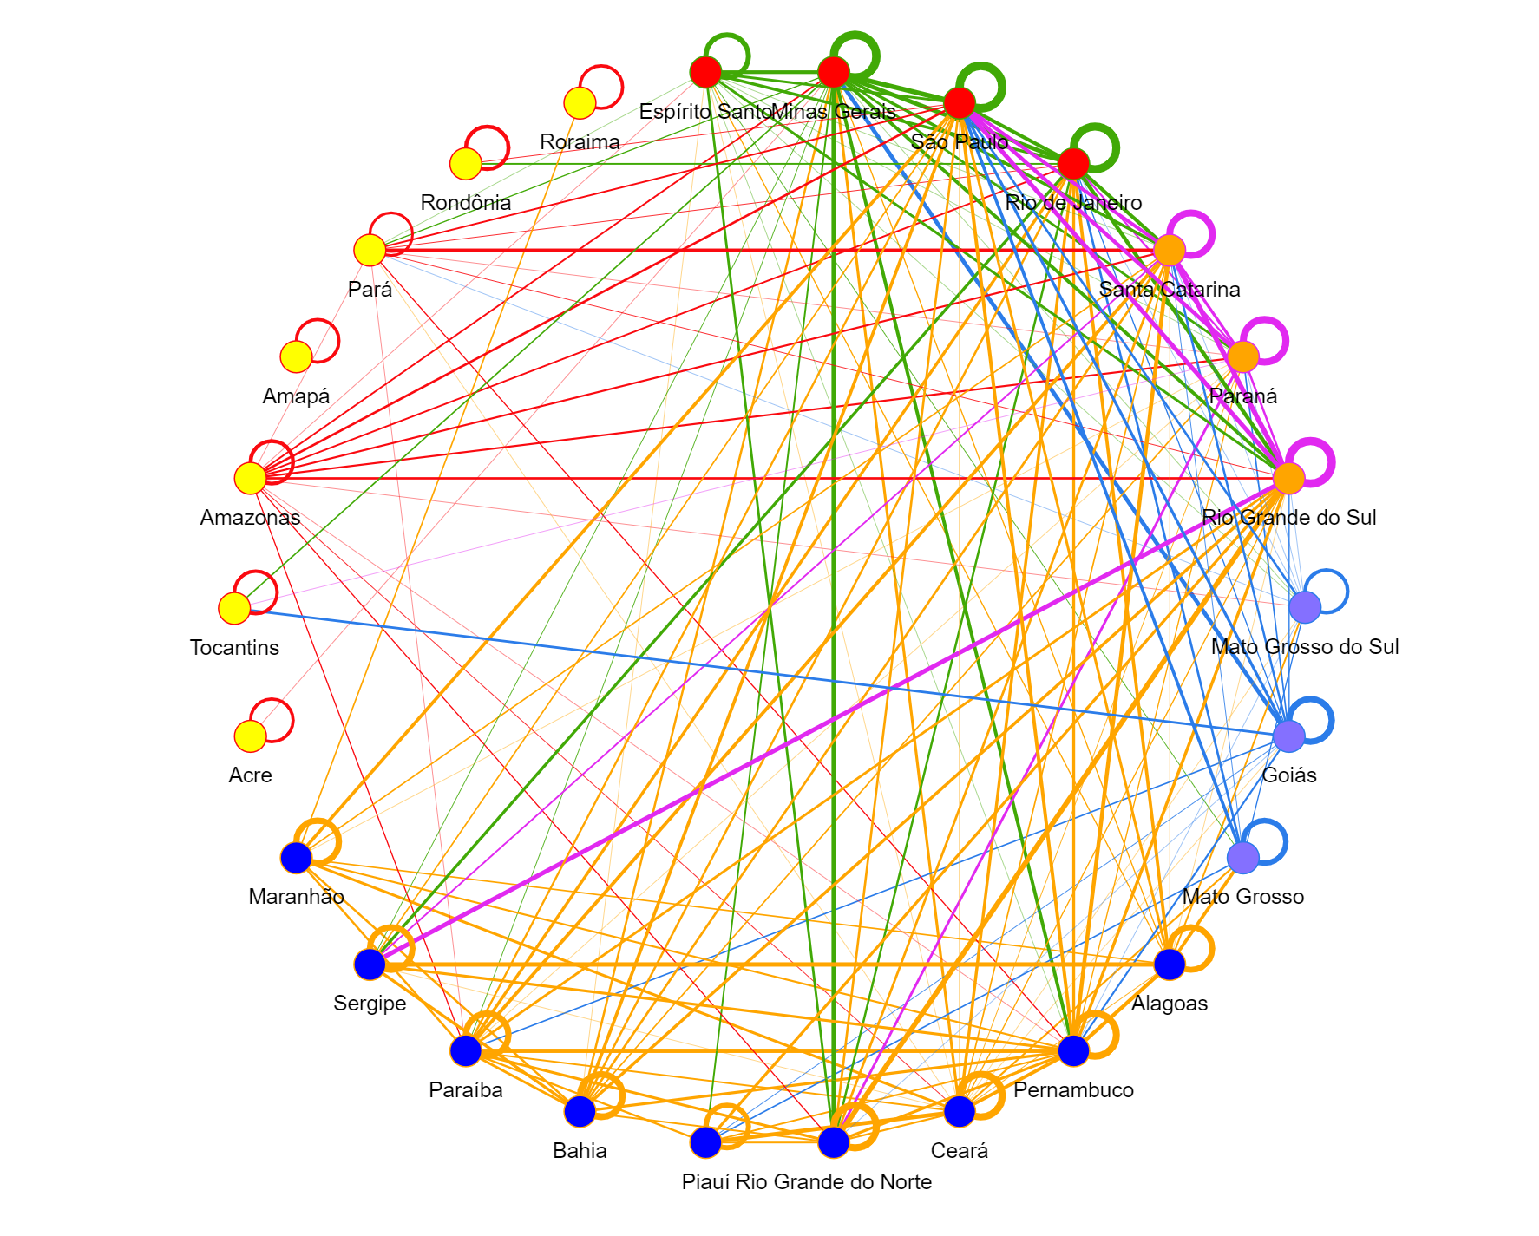
\includegraphics[scale=0.6]{Imagens/rede-2012.pdf}
	\caption{Rede de Coautoria das Universidades Federais do Brasil (\textit{Health Sciences}) - 2012}
	\label{Rede de Coautoria - UF BR 2012}
\end{figure}

\begin{figure}[H]
	\centering
	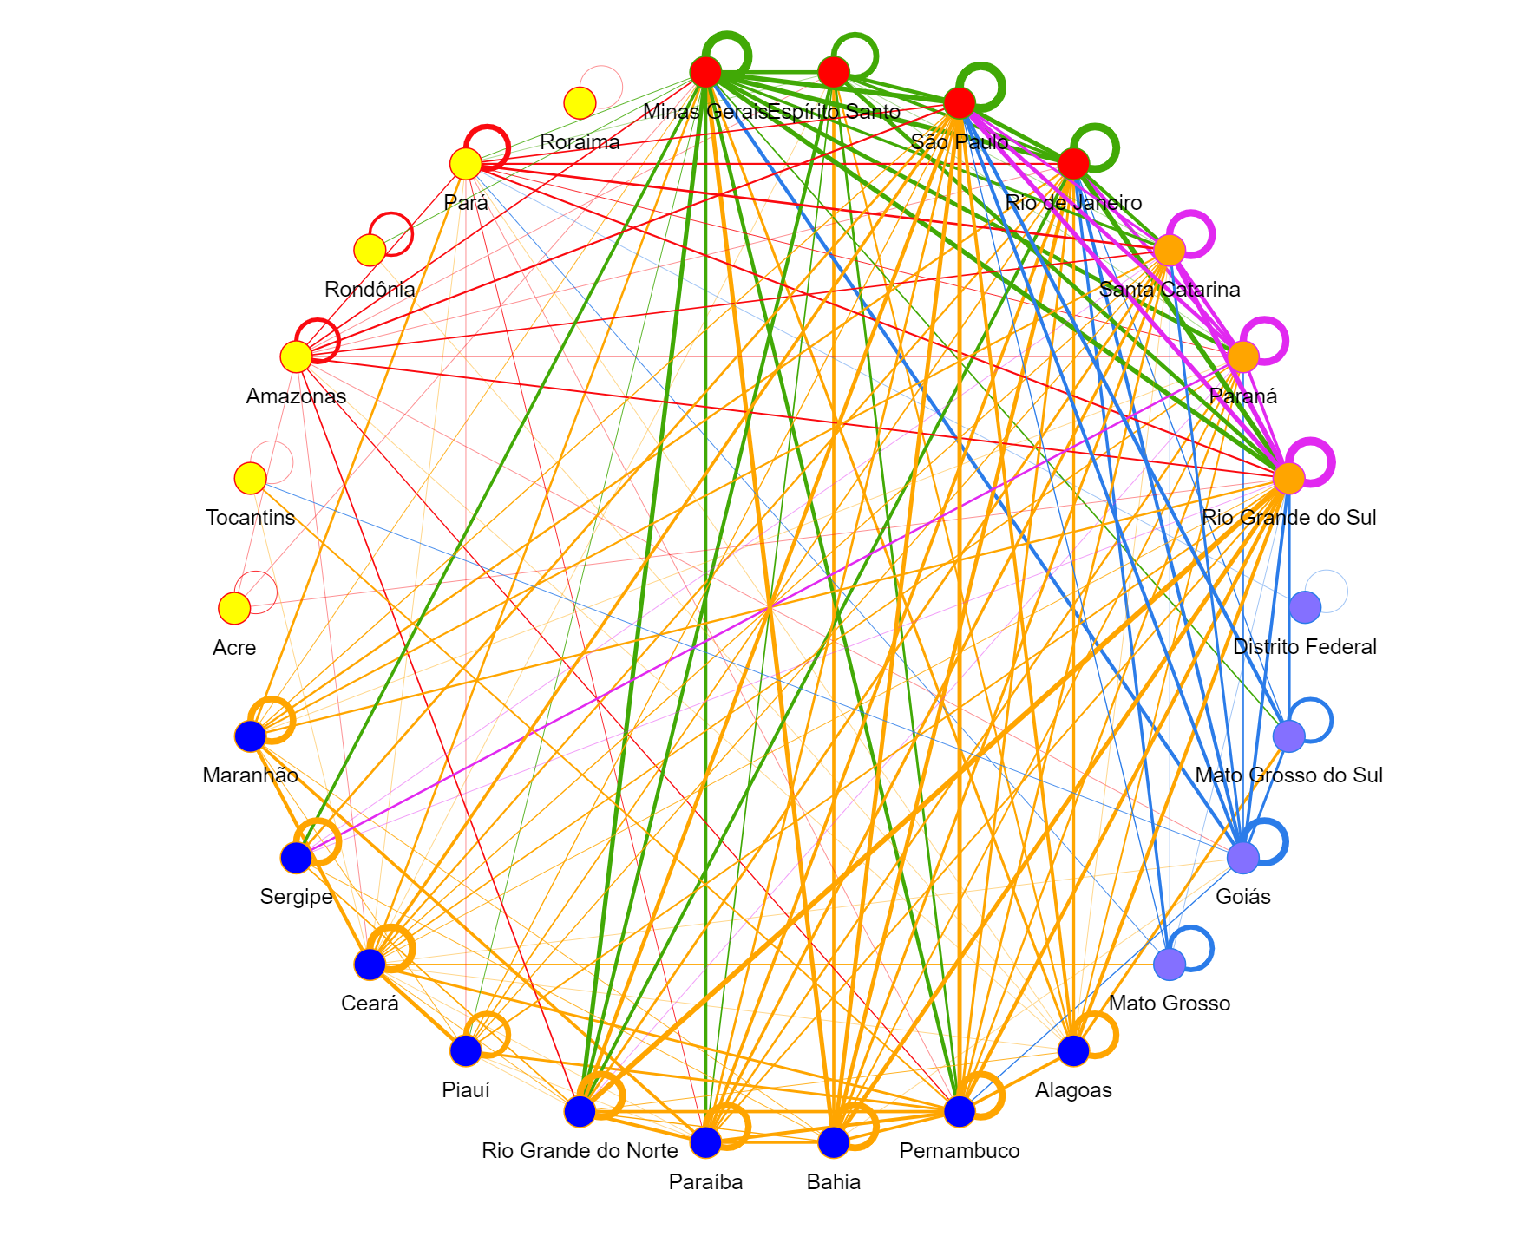
\includegraphics[scale=0.6]{Imagens/rede-2013.pdf}
	\caption{Rede de Coautoria das Universidades Federais do Brasil (\textit{Health Sciences}) - 2013}
	\label{Rede de Coautoria - UF BR 2013}
\end{figure}

\begin{figure}[H]
	\centering
	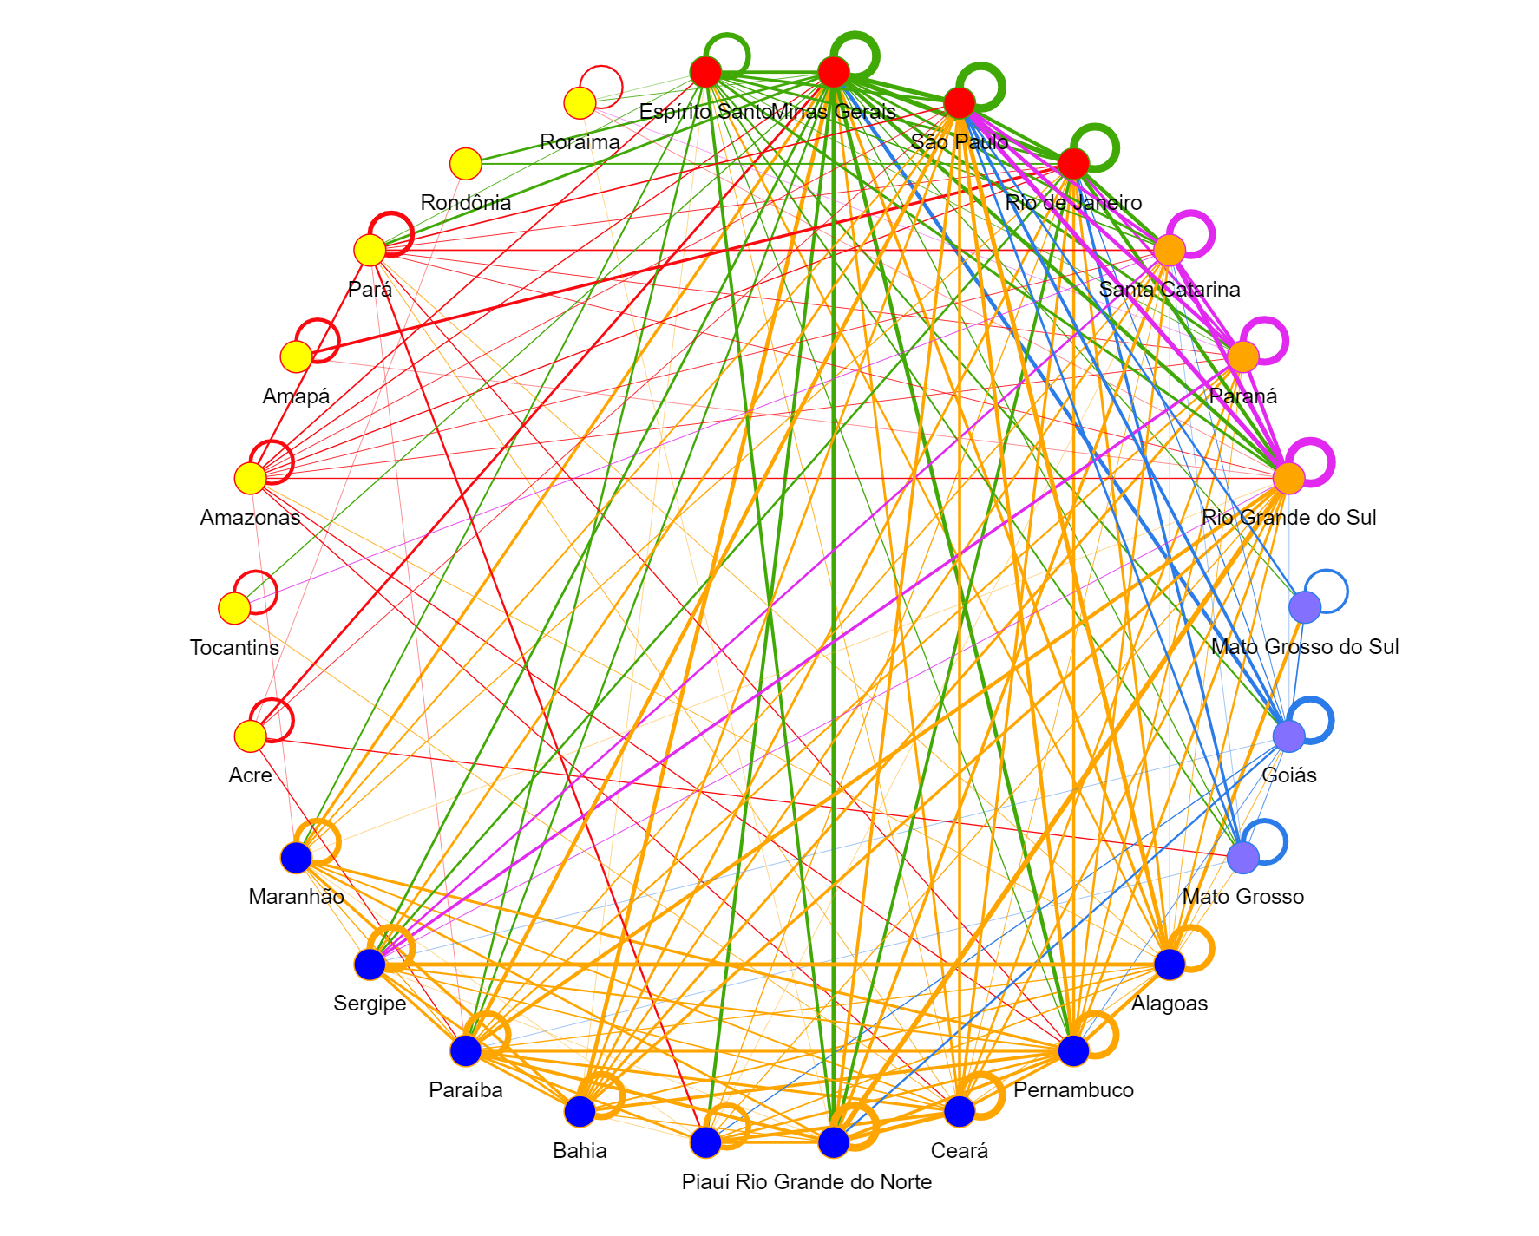
\includegraphics[scale=0.6]{Imagens/rede-2014.pdf}
	\caption{Rede de Coautoria das Universidades Federais do Brasil (\textit{Health Sciences}) - 2014}
	\label{Rede de Coautoria - UF BR 2014}
\end{figure}


\begin{figure}[H]
	\centering
	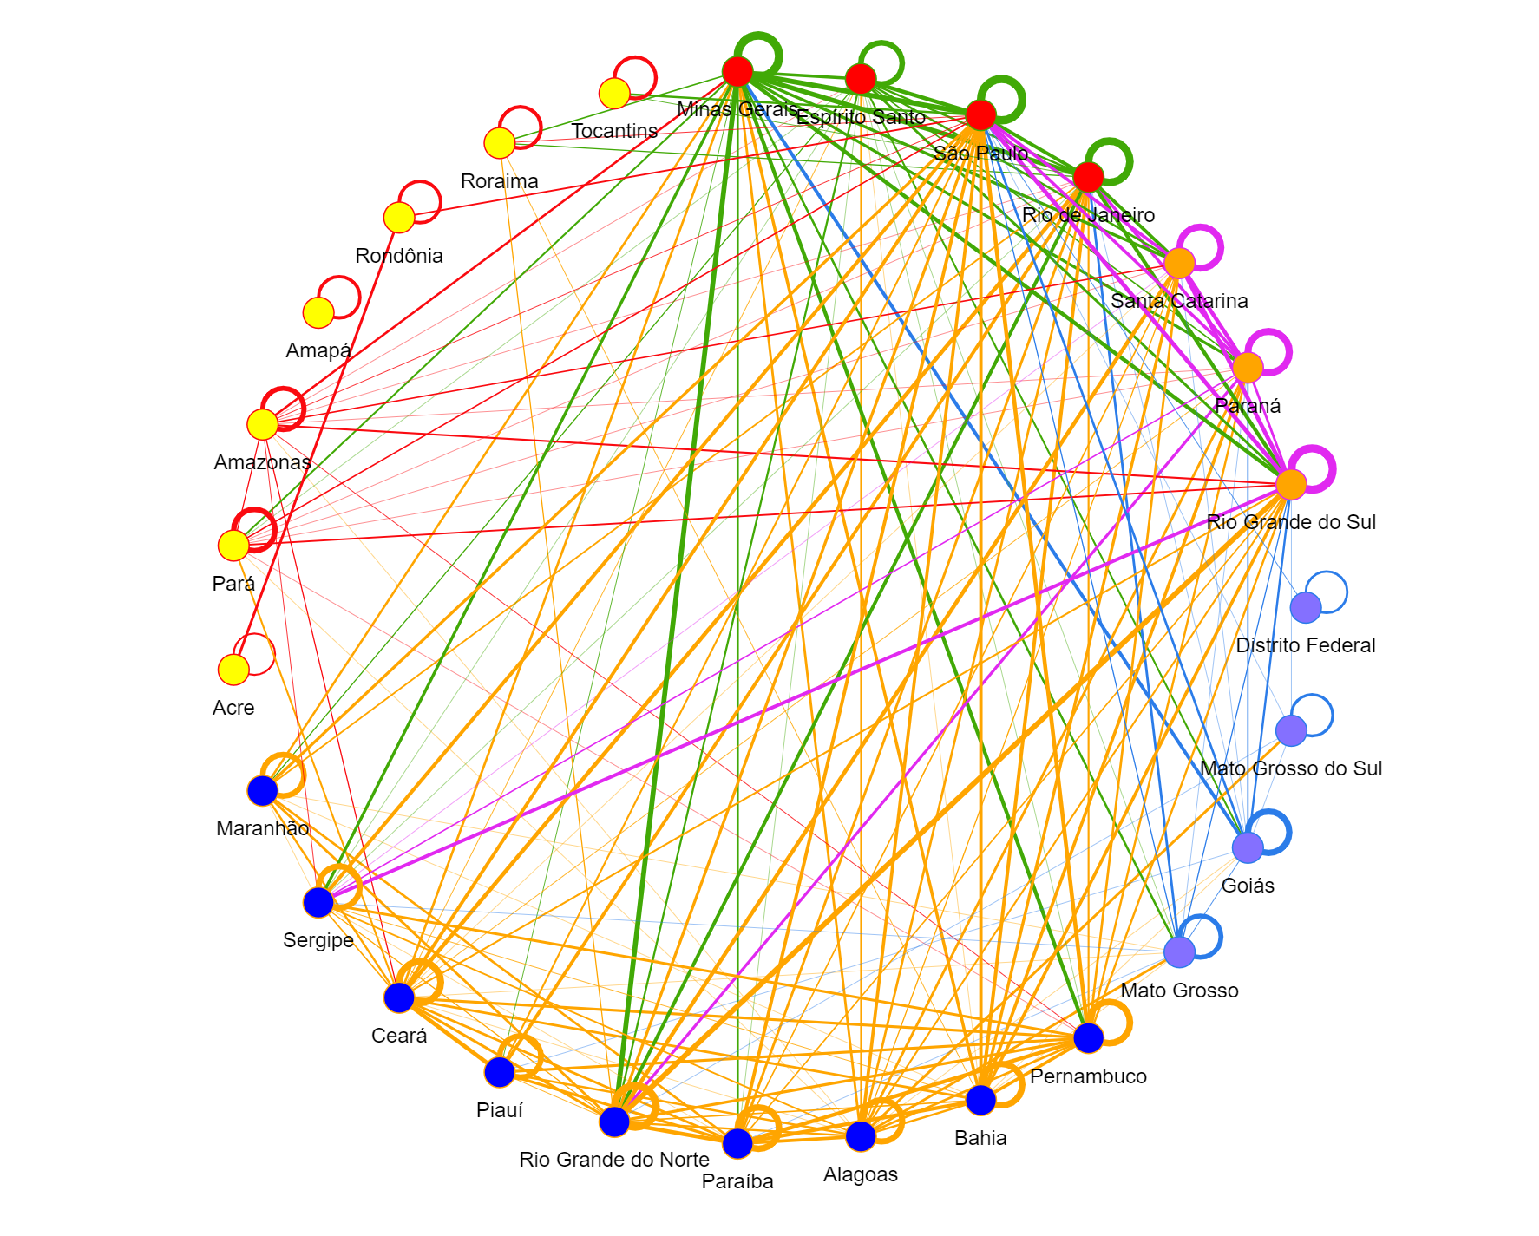
\includegraphics[scale=0.6]{Imagens/rede-2015.pdf}
	\caption{Rede de Coautoria das Universidades Federais do Brasil (\textit{Health Sciences}) - 2015}
	\label{Rede de Coautoria - UF BR 2015}
\end{figure}

\begin{figure}[H]
	\centering
	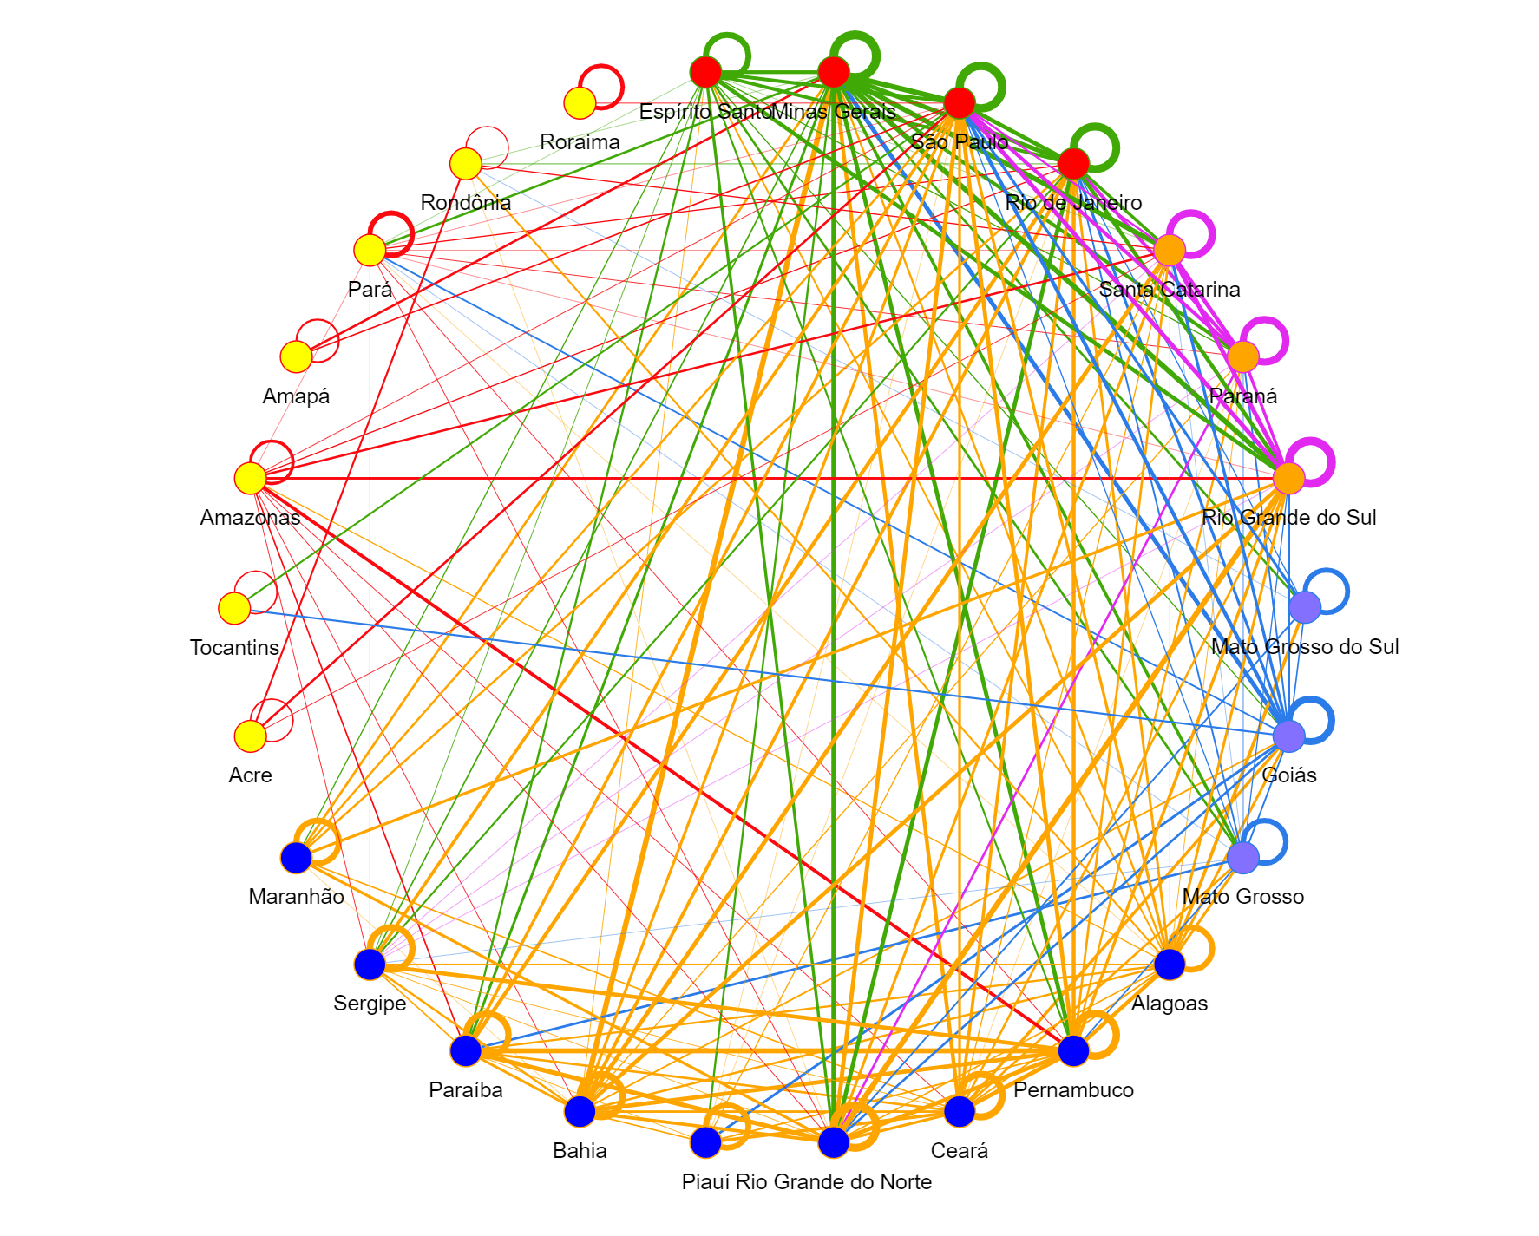
\includegraphics[scale=0.6]{Imagens/rede-2016.pdf}
	\caption{Rede de Coautoria das Universidades Federais do Brasil (\textit{Health Sciences}) - 2016}
	\label{Rede de Coautoria - UF BR 2016}
\end{figure}

\begin{figure}[H]
	\centering
	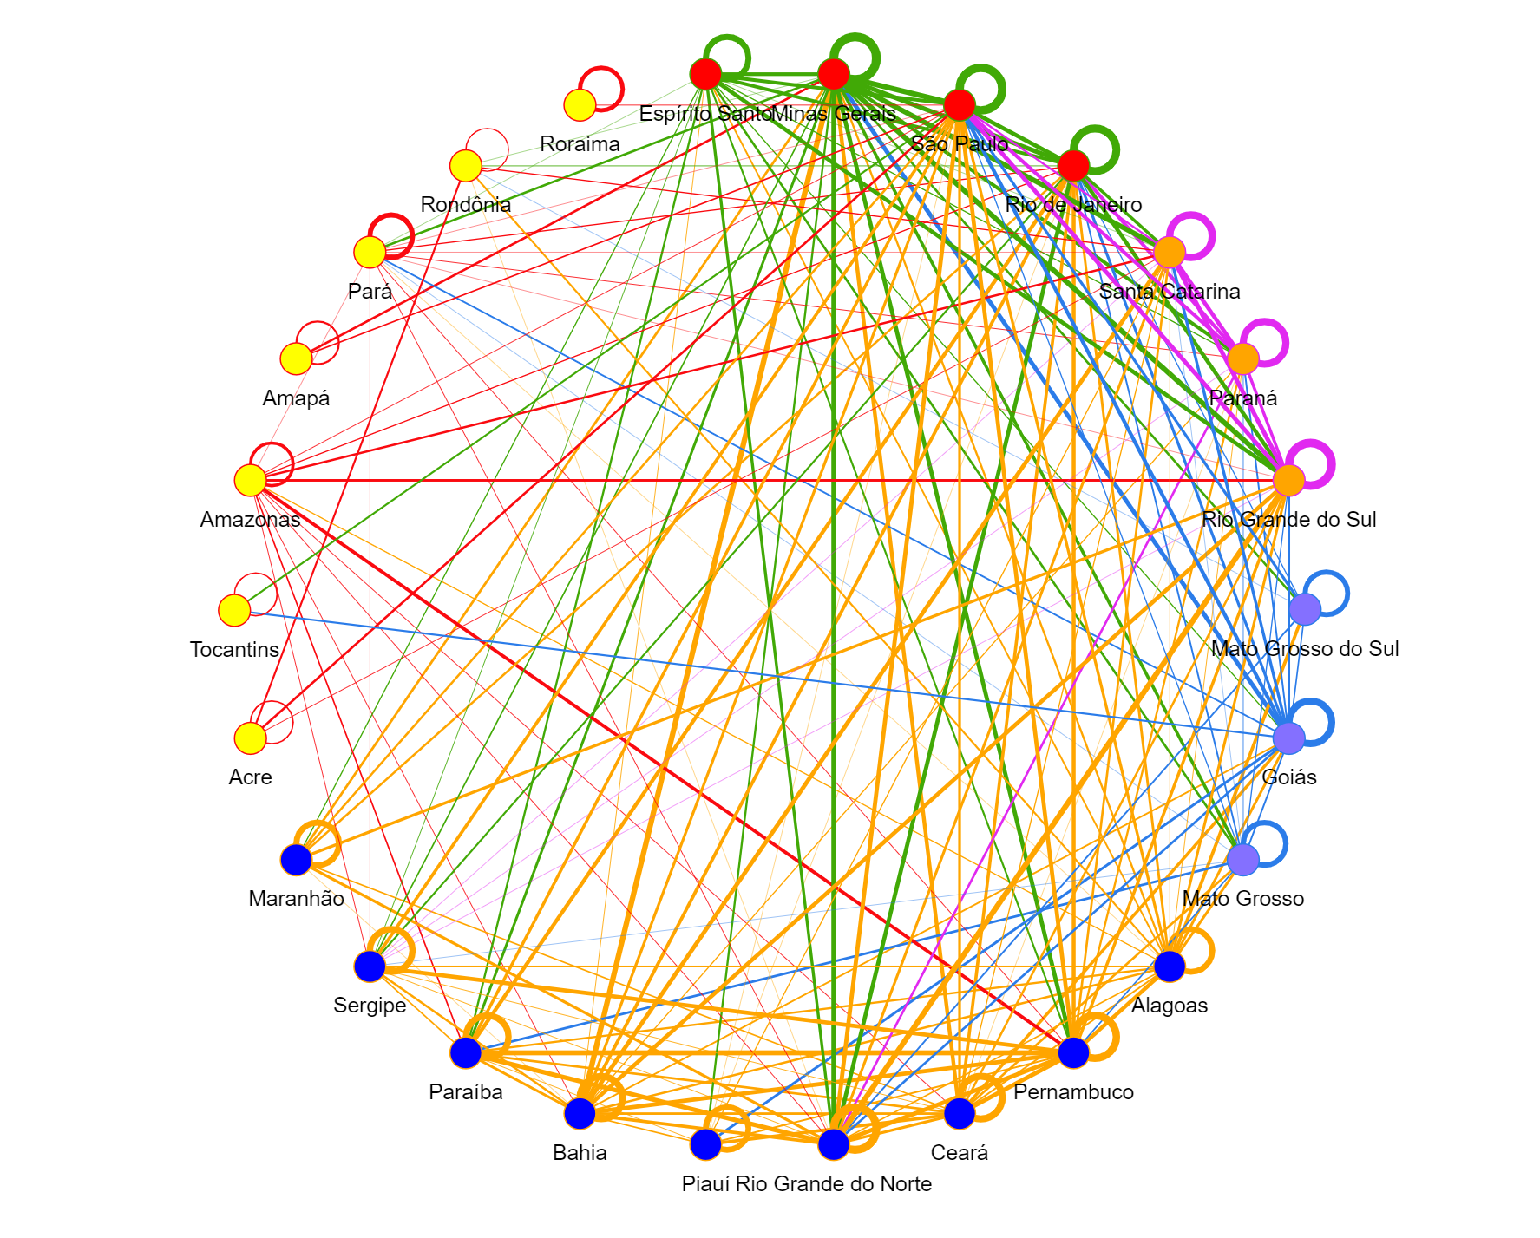
\includegraphics[scale=0.6]{Imagens/rede-2017.pdf}
	\caption{Rede de Coautoria das Universidades Federais do Brasil (\textit{Health Sciences}) - 2017}
	\label{Rede de Coautoria - UF BR 2017}
\end{figure}

\subsubsection{Redes de Coautoria Brasil - Vértice Focal Alagoas - Área: \textit{Health Sciences}}

\begin{figure}[H]
	\centering
	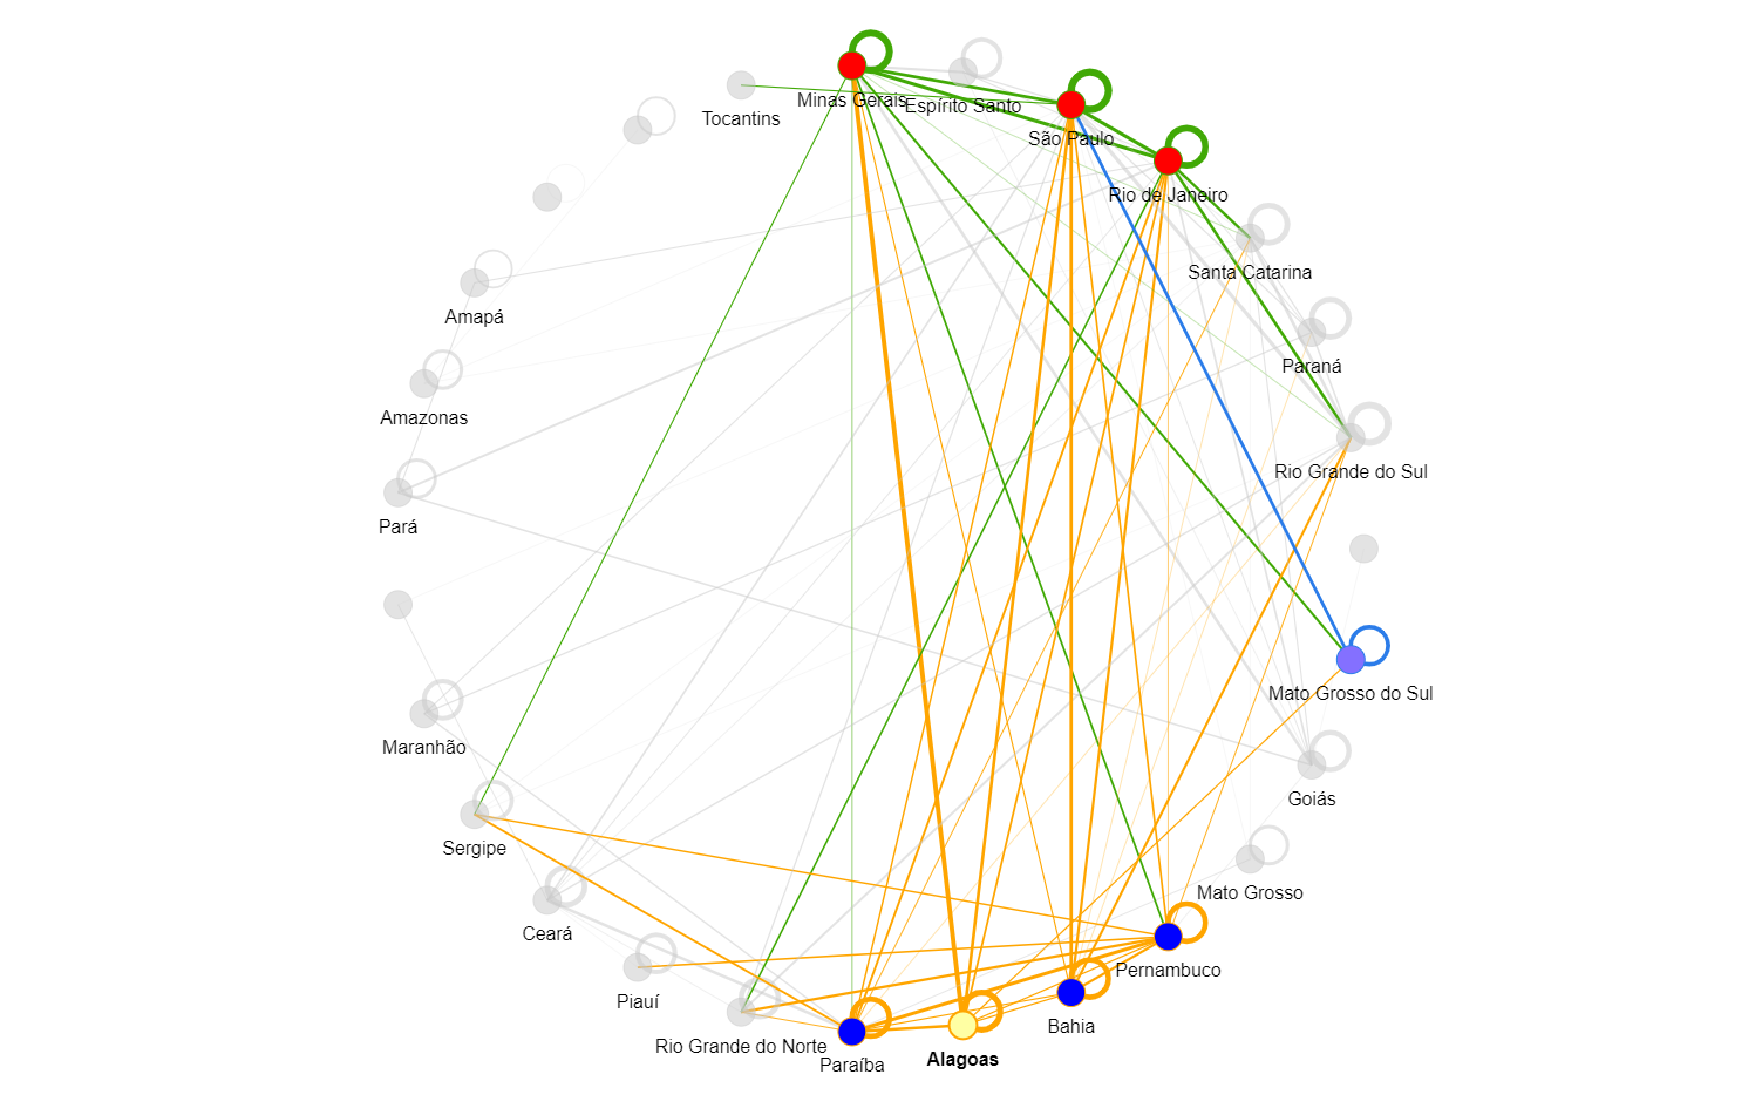
\includegraphics[scale=0.6]{Imagens/rede-al-2008.pdf}
	\caption{Rede de Coautoria da Universidade Federal de Alagoas (\textit{Health Sciences}) - 2008}
	\label{Rede de Coautoria - UF AL 2008}
\end{figure}

\begin{figure}[H]
	\centering
	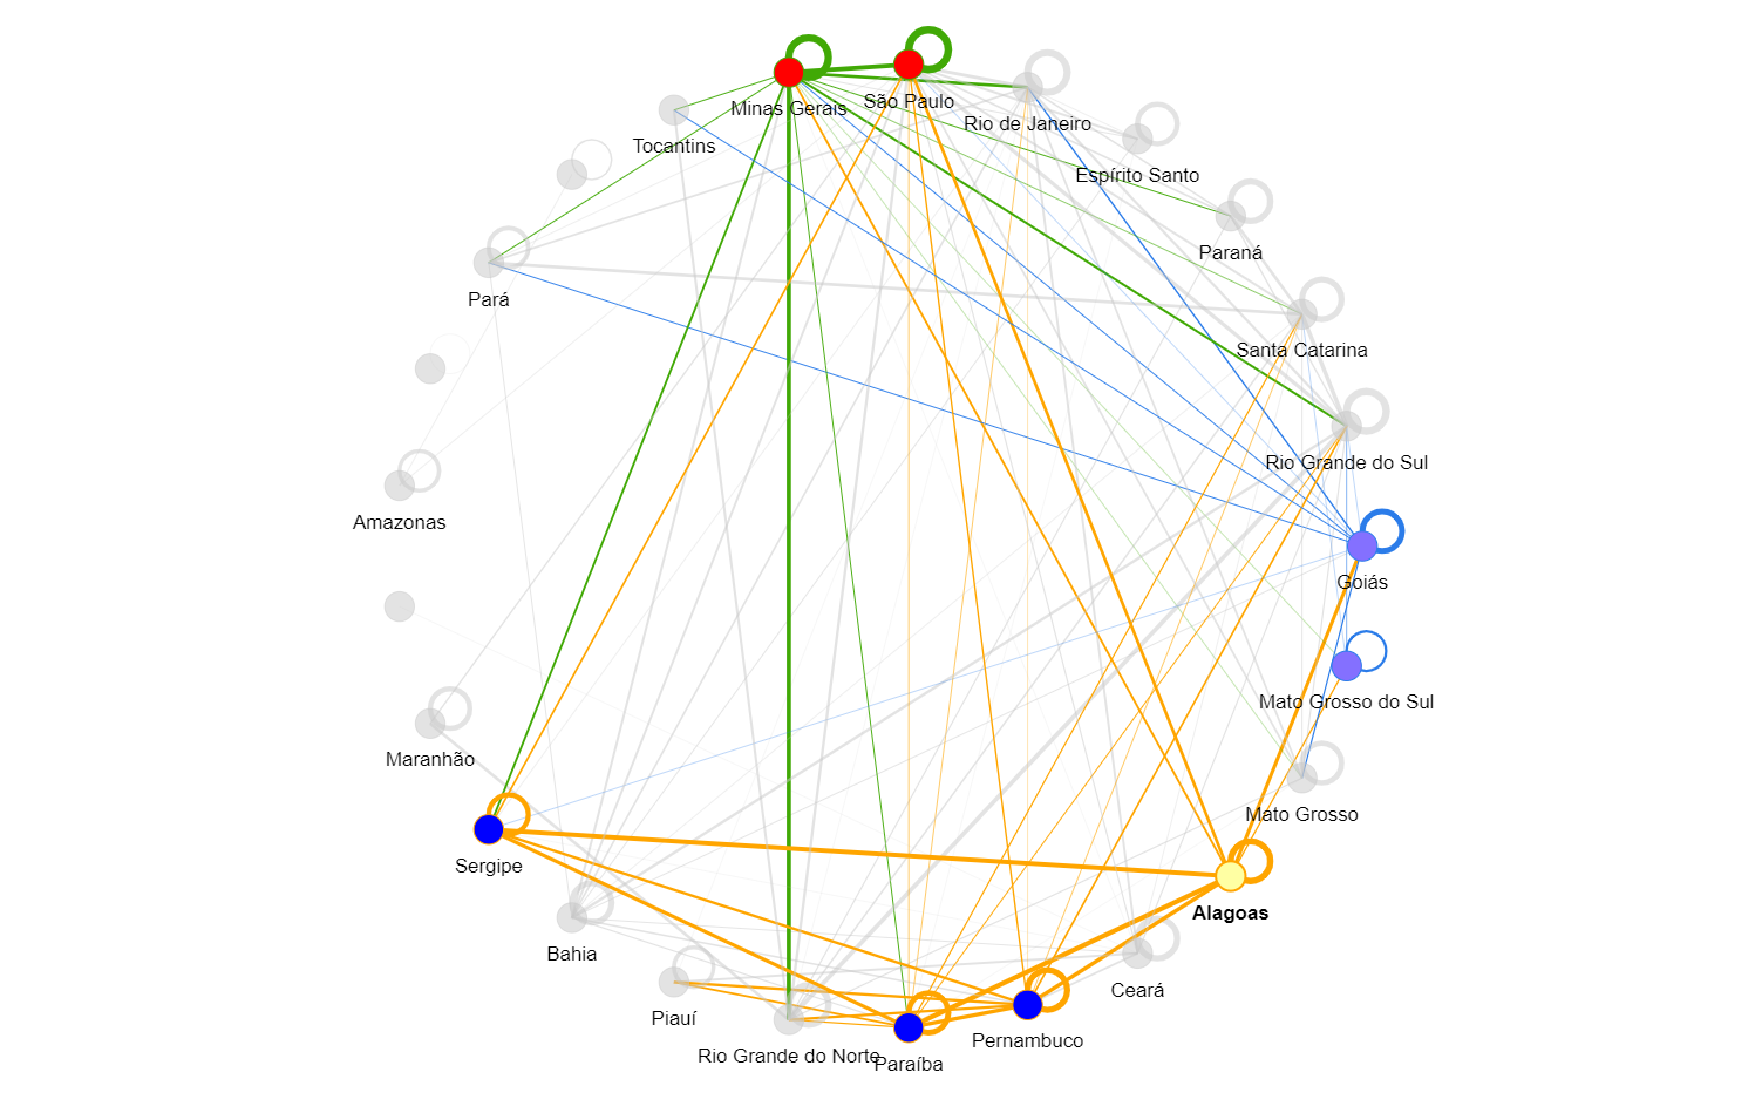
\includegraphics[scale=0.6]{Imagens/rede-al-2009.pdf}
	\caption{Rede de Coautoria da Universidade Federal de Alagoas (\textit{Health Sciences}) - 2009}
	\label{Rede de Coautoria - UF AL 2009}
\end{figure}

\begin{figure}[H]
	\centering
	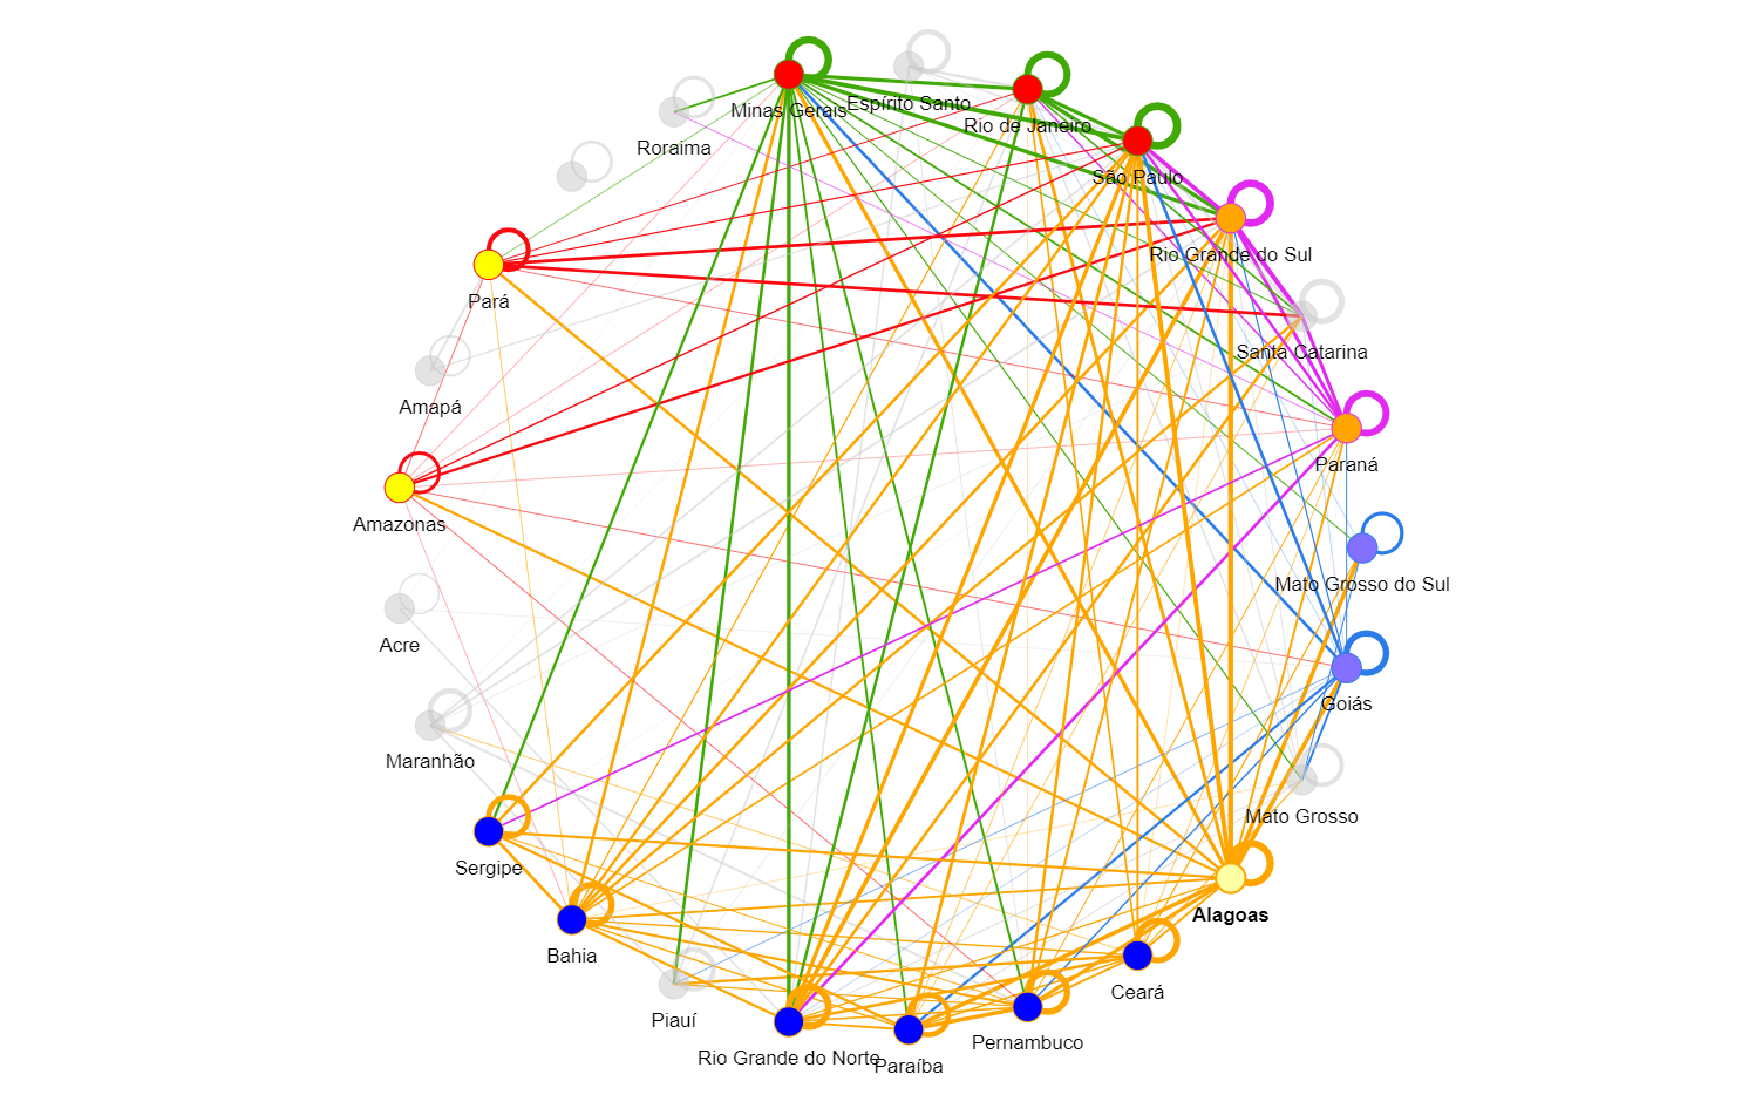
\includegraphics[scale=0.6]{Imagens/rede-al-2010.pdf}
	\caption{Rede de Coautoria da Universidade Federal de Alagoas (\textit{Health Sciences}) - 2010}
	\label{Rede de Coautoria - UF AL 2010}
\end{figure}

\begin{figure}[H]
	\centering
	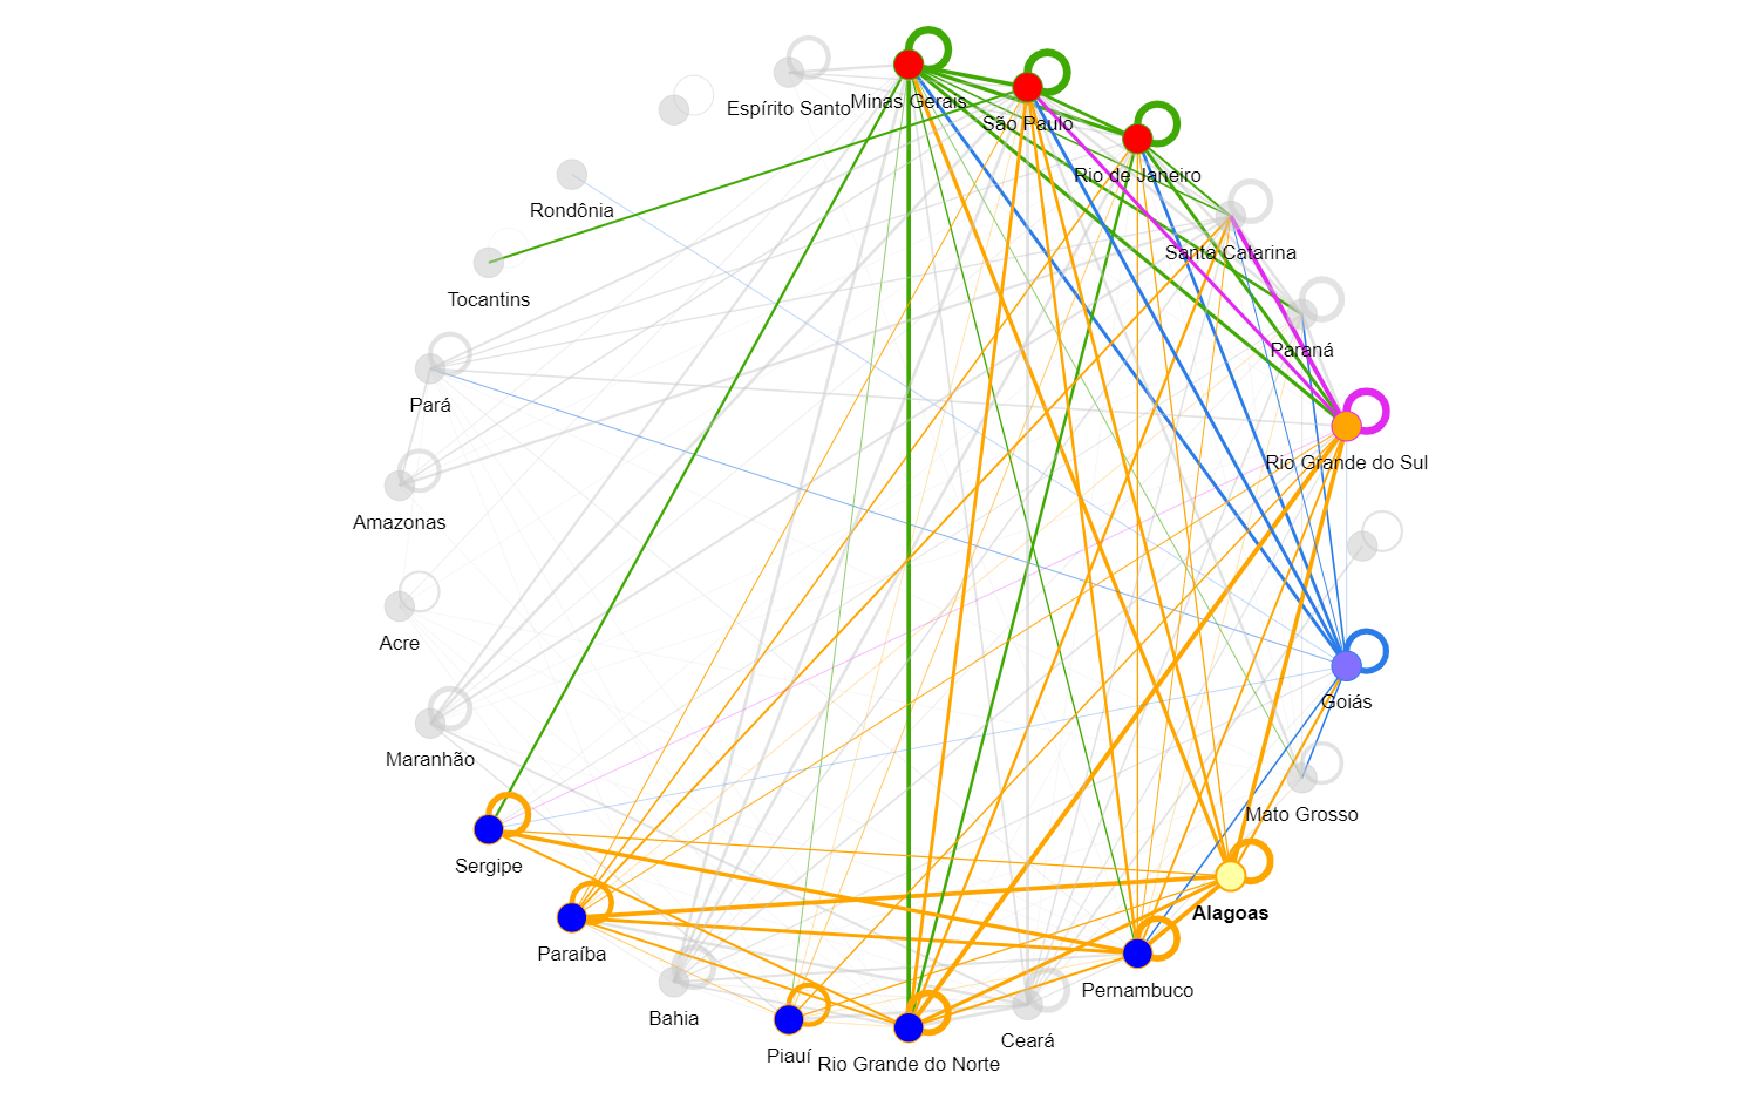
\includegraphics[scale=0.6]{Imagens/rede-al-2011.pdf}
	\caption{Rede de Coautoria da Universidade Federal de Alagoas (\textit{Health Sciences}) - 2011}
	\label{Rede de Coautoria - UF AL 2011}
\end{figure}


\begin{figure}[H]
	\centering
	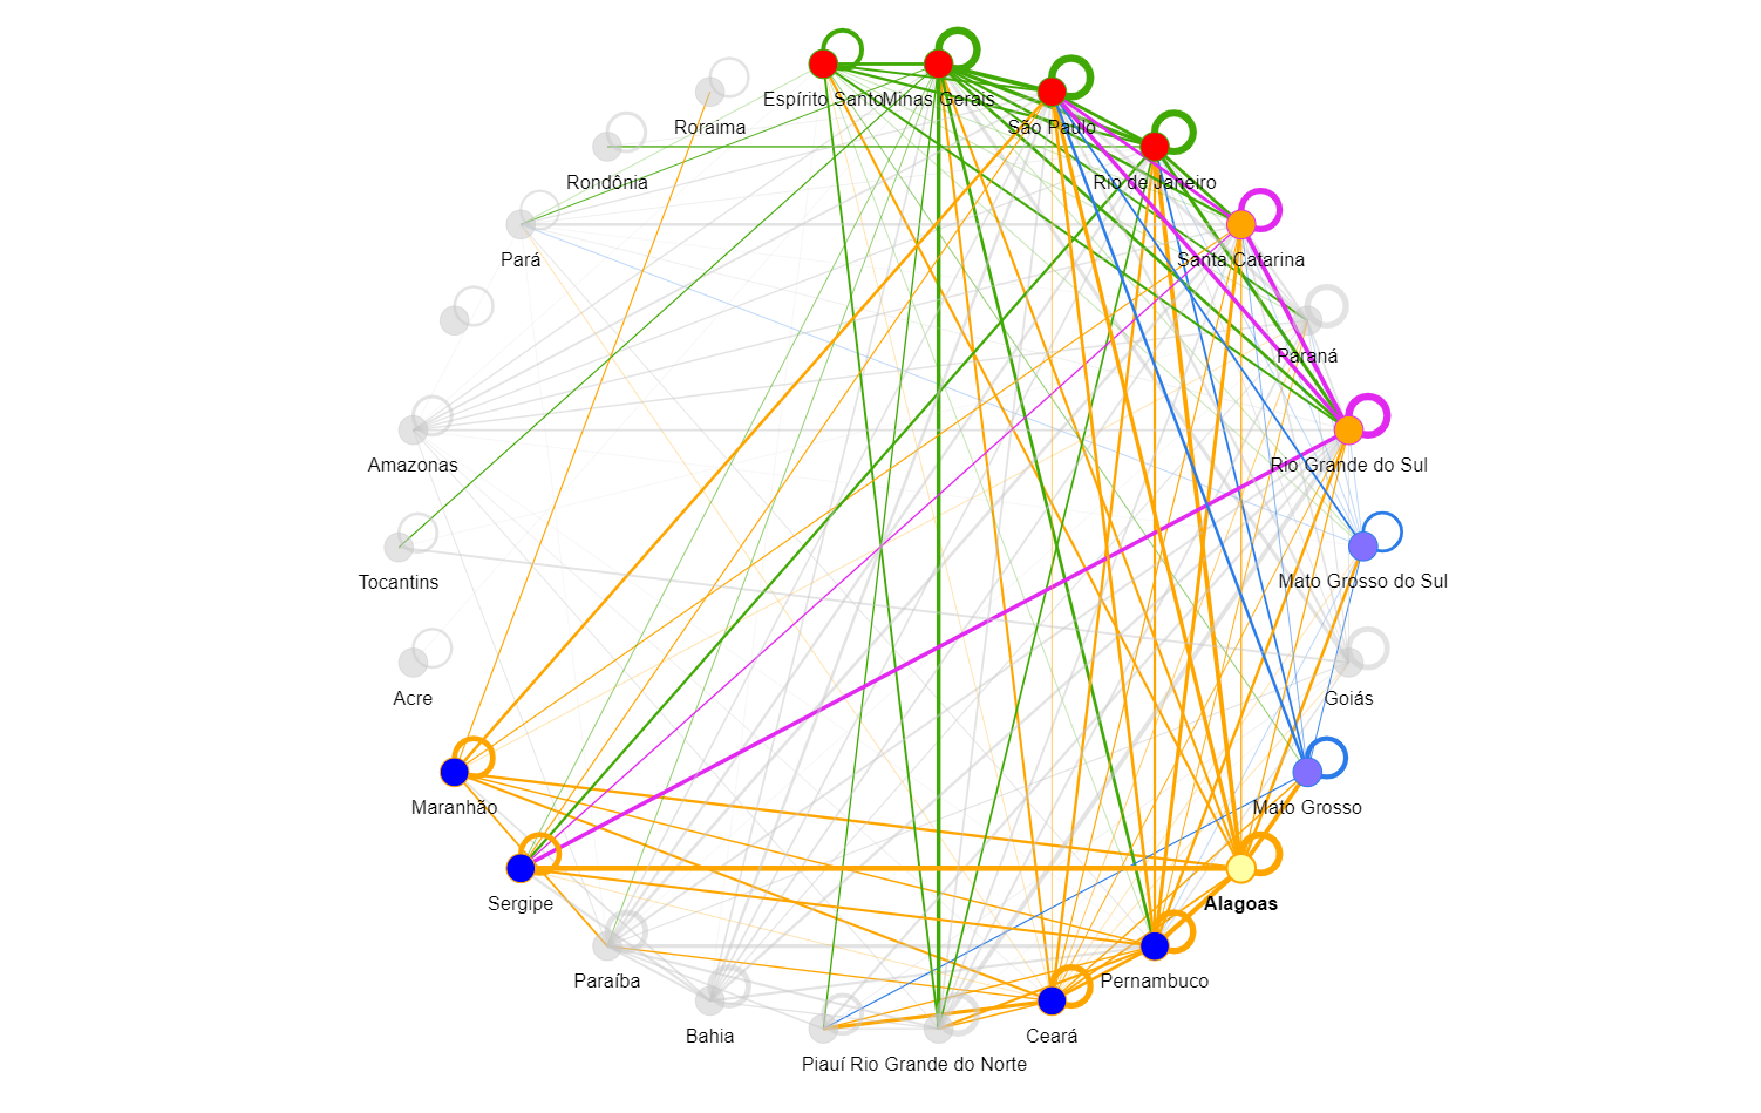
\includegraphics[scale=0.6]{Imagens/rede-al-2012.pdf}
	\caption{Rede de Coautoria da Universidade Federal de Alagoas (\textit{Health Sciences}) - 2012}
	\label{Rede de Coautoria - UF AL 2012}
\end{figure}

\begin{figure}[H]
	\centering
	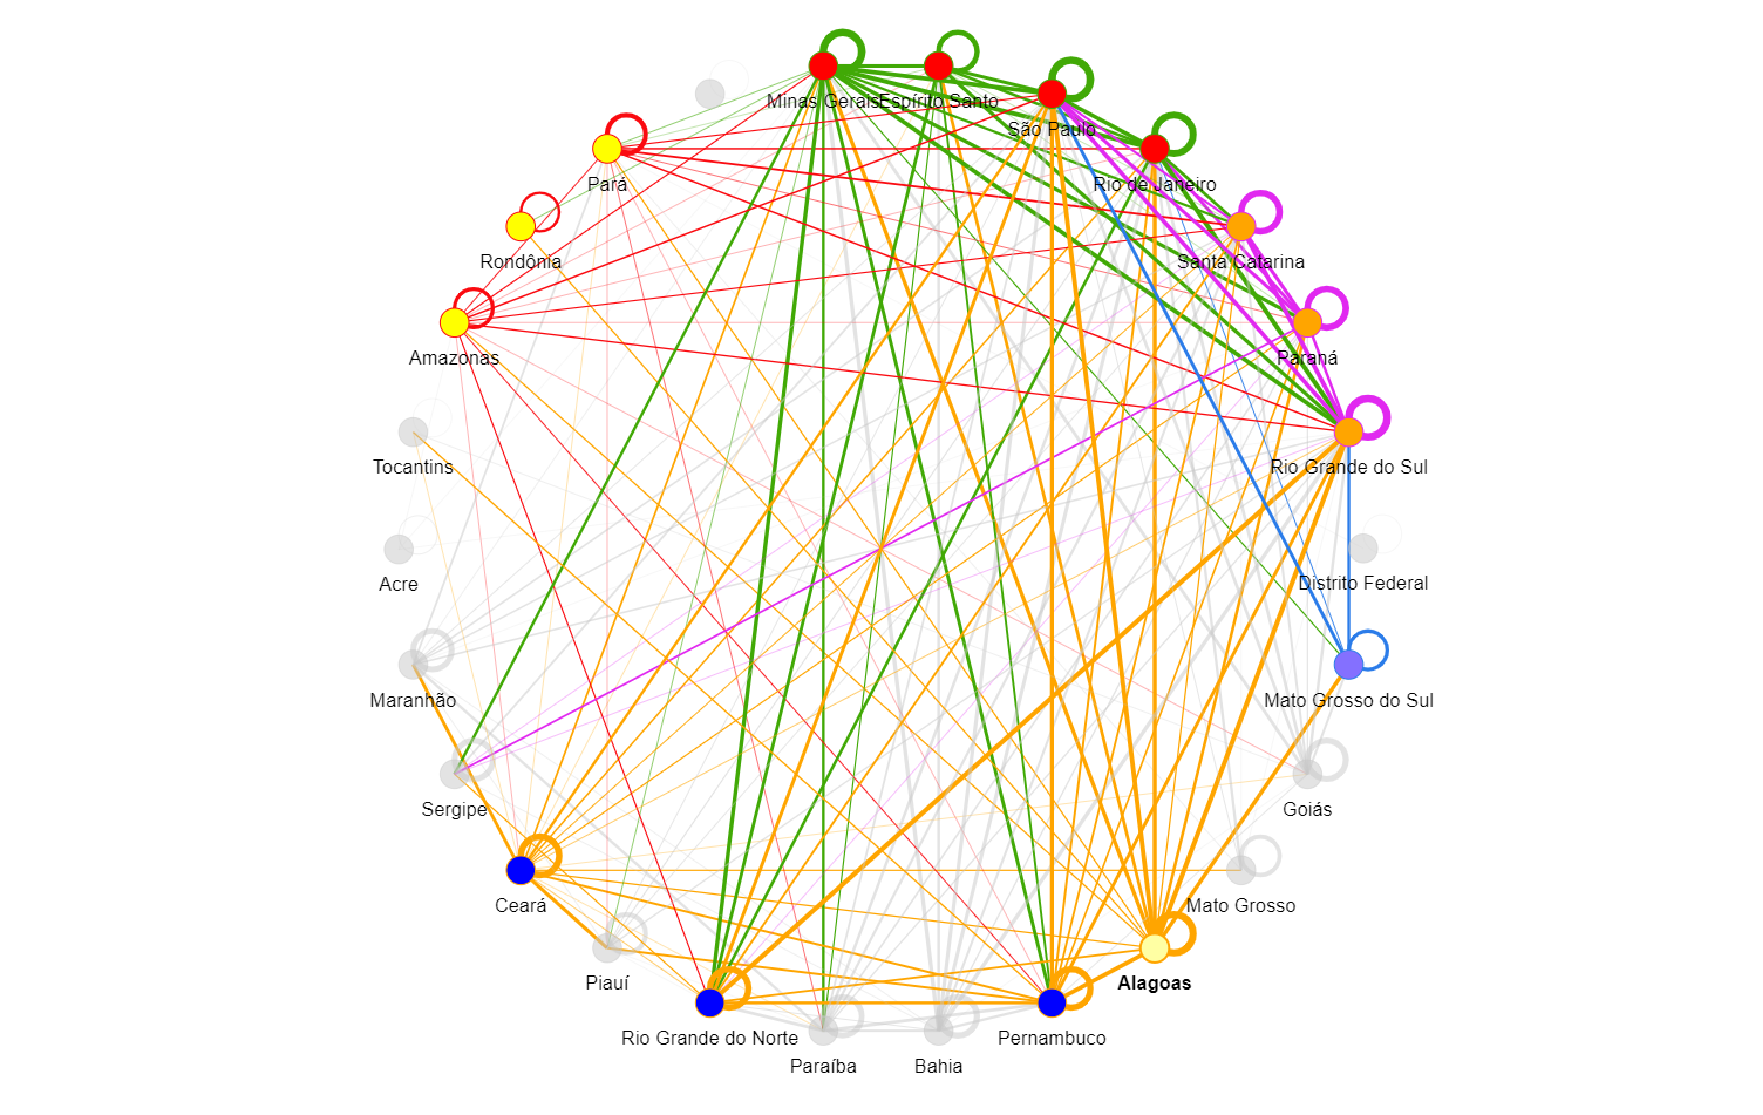
\includegraphics[scale=0.6]{Imagens/rede-al-2013.pdf}
	\caption{Rede de Coautoria da Universidade Federal de Alagoas (\textit{Health Sciences}) - 2013}
	\label{Rede de Coautoria - UF AL 2013}
\end{figure}

\begin{figure}[H]
	\centering
	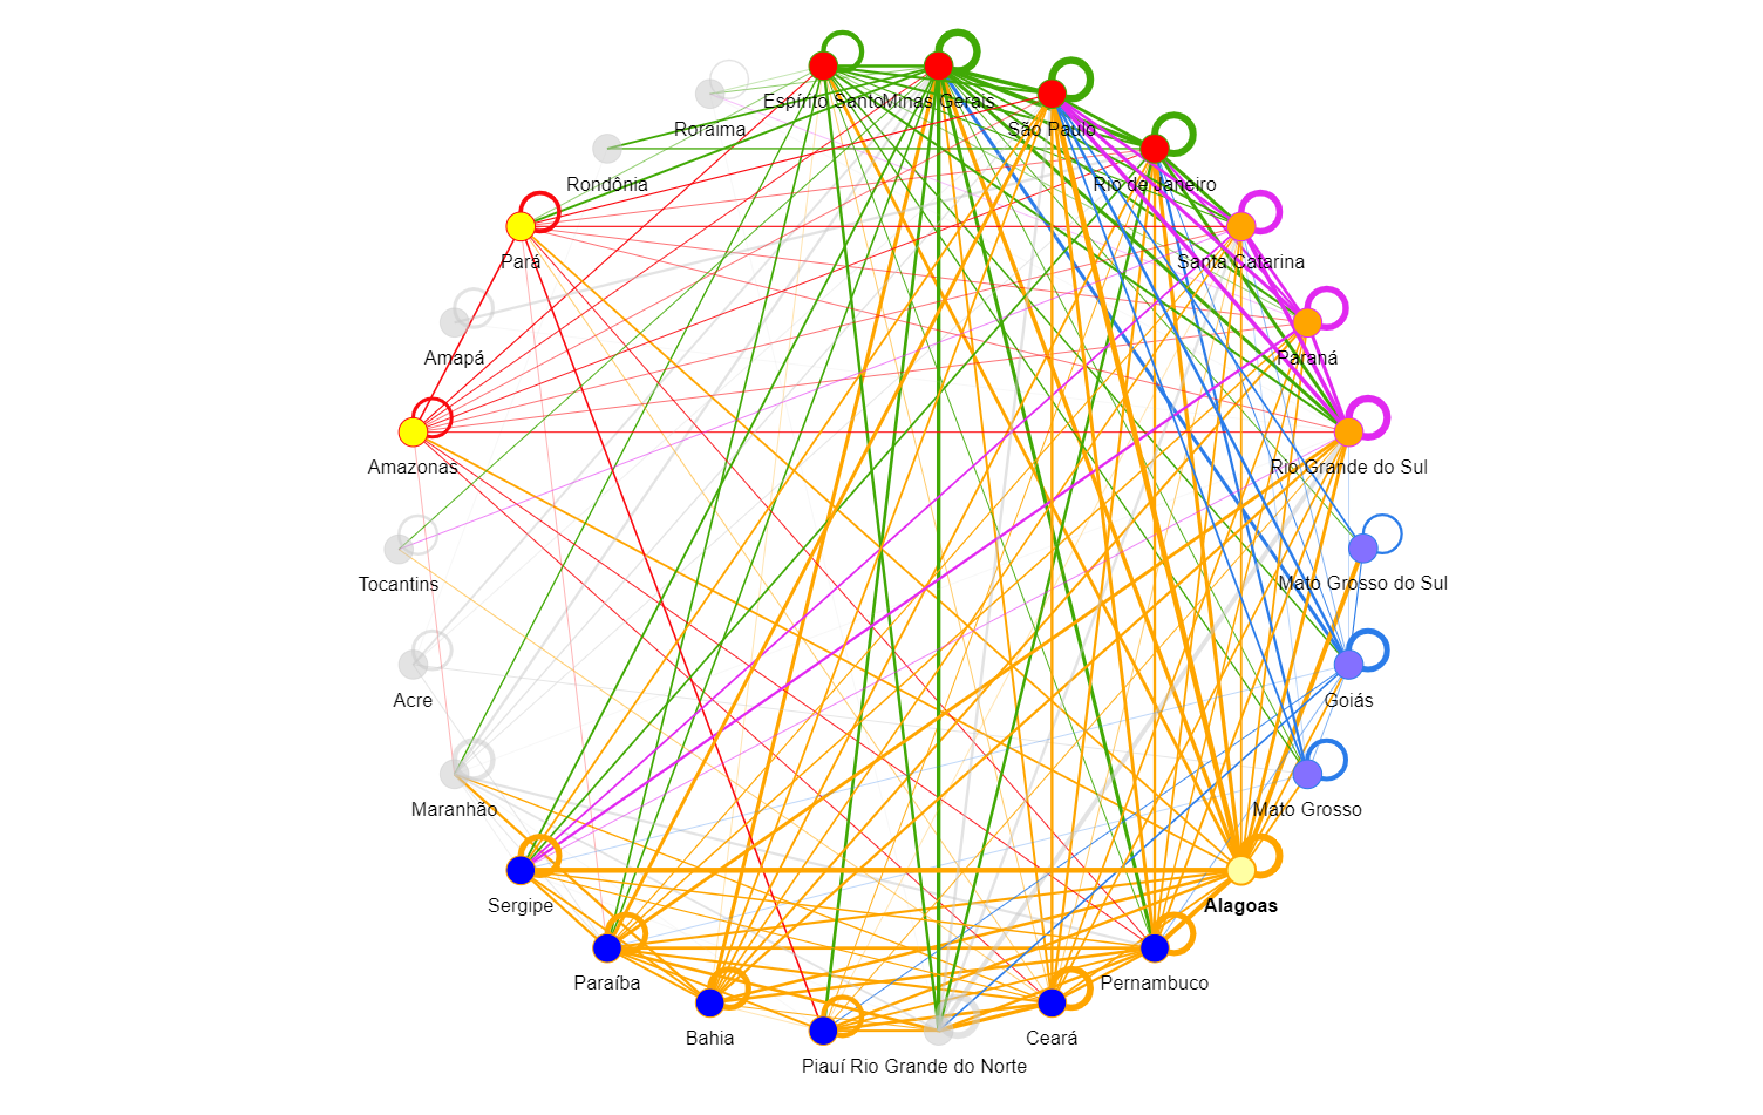
\includegraphics[scale=0.6]{Imagens/rede-al-2014.pdf}
	\caption{Rede de Coautoria da Universidade Federal de Alagoas (\textit{Health Sciences}) - 2014}
	\label{Rede de Coautoria - UF AL 2014}
\end{figure}


\begin{figure}[H]
	\centering
	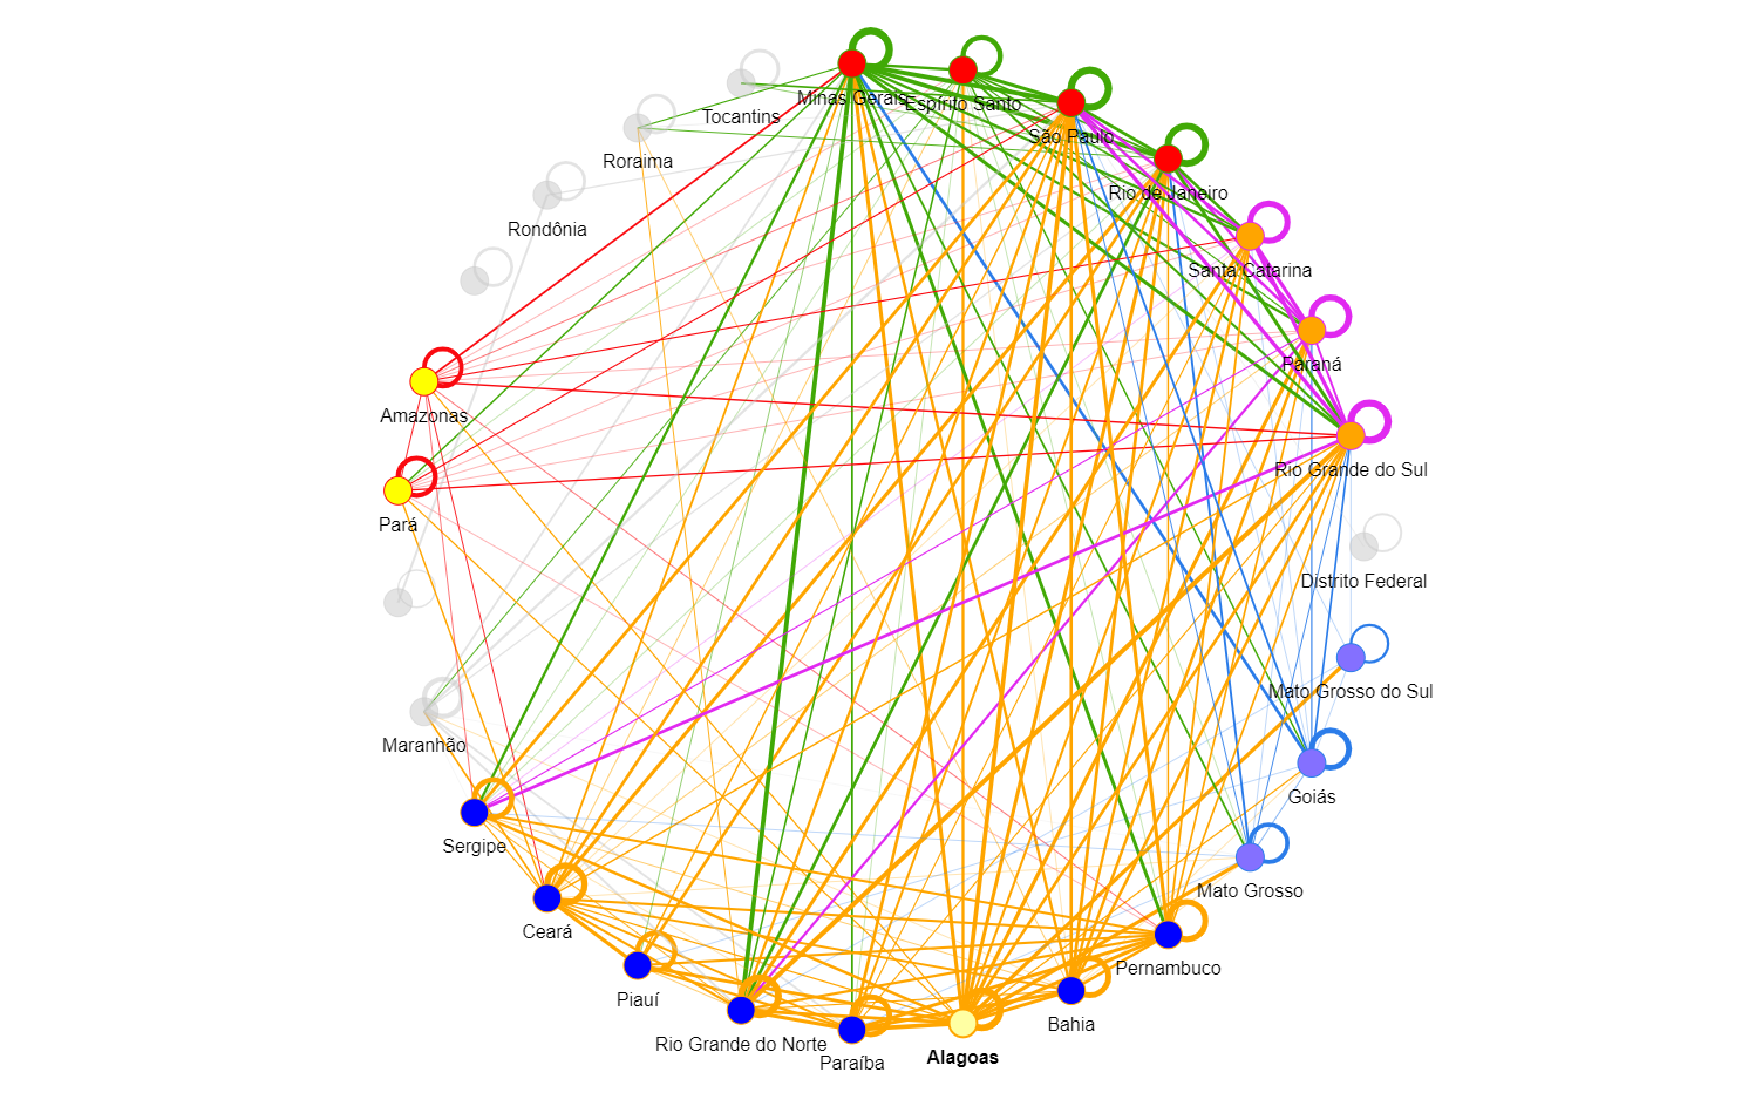
\includegraphics[scale=0.6]{Imagens/rede-al-2015.pdf}
	\caption{Rede de Coautoria da Universidade Federal de Alagoas (\textit{Health Sciences}) - 2015}
	\label{Rede de Coautoria - UF AL 2015}
\end{figure}

\begin{figure}[H]
	\centering
	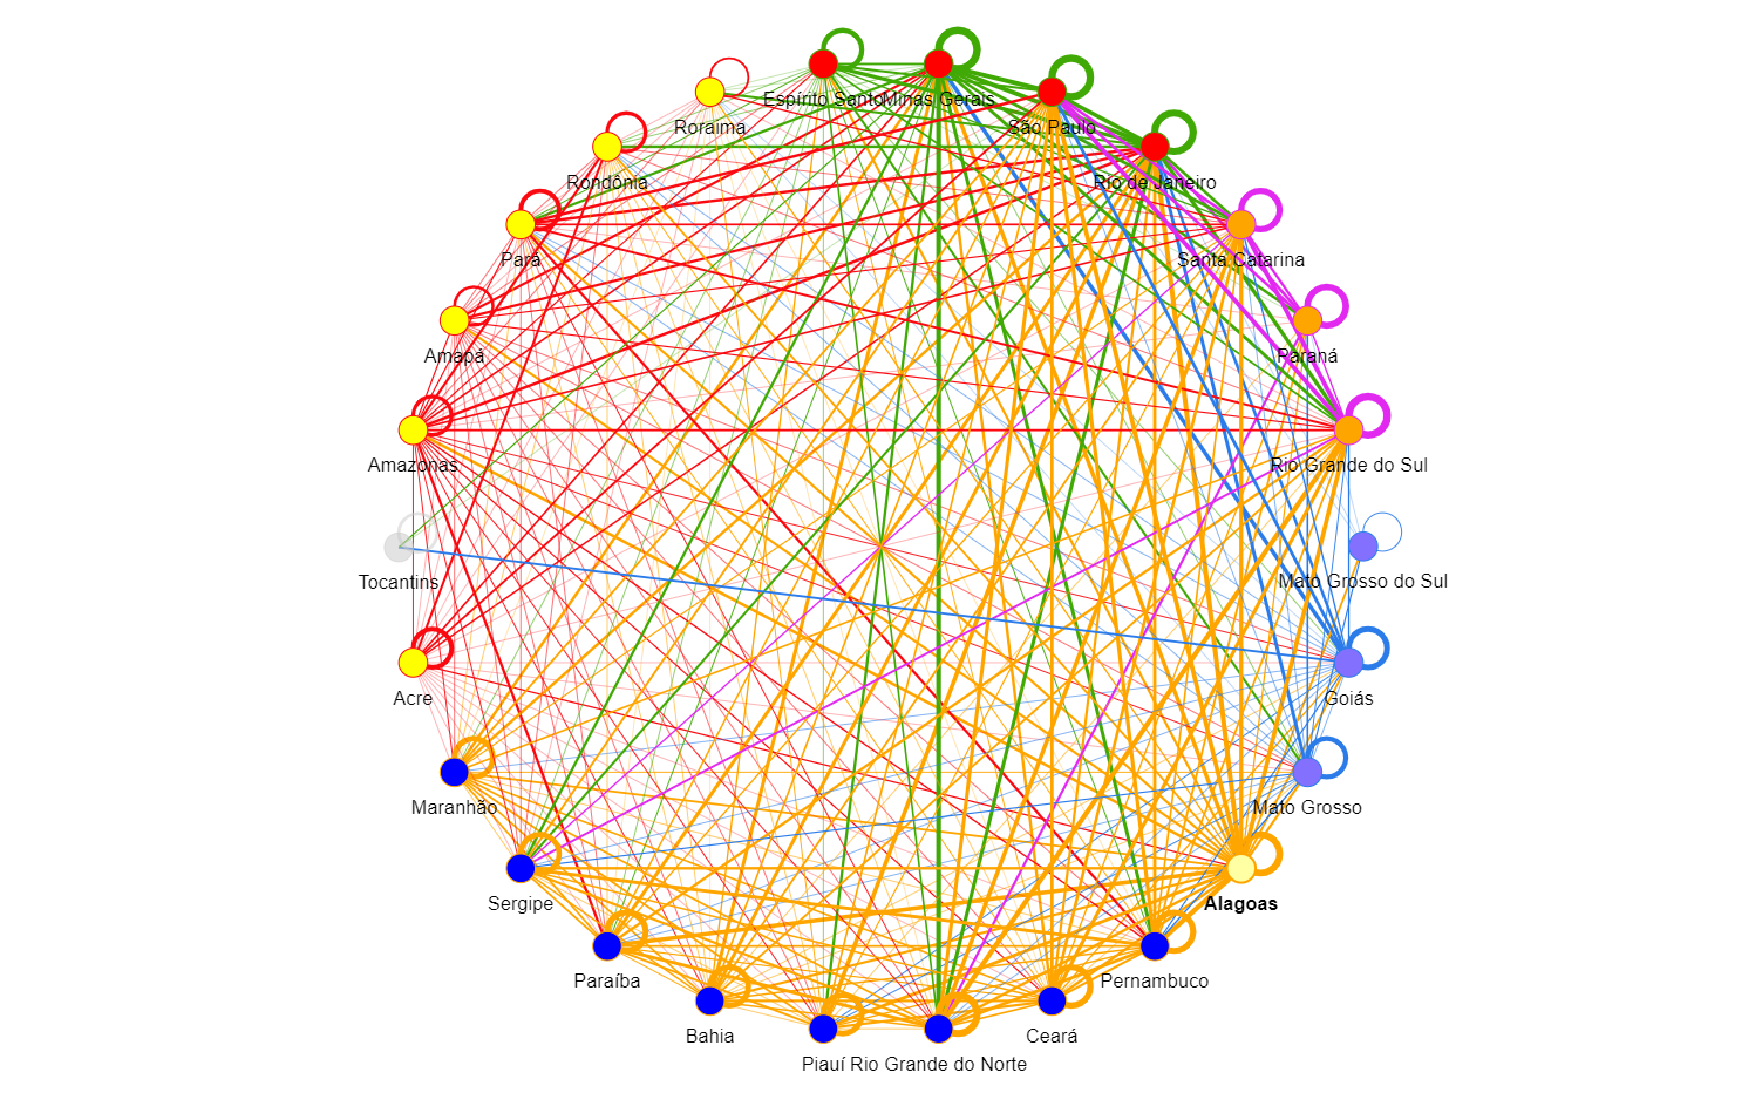
\includegraphics[scale=0.6]{Imagens/rede-al-2016.pdf}
	\caption{Rede de Coautoria da Universidade Federal de Alagoas (\textit{Health Sciences}) - 2016}
	\label{Rede de Coautoria - UF AL 2016}
\end{figure}

\begin{figure}[H]
	\centering
	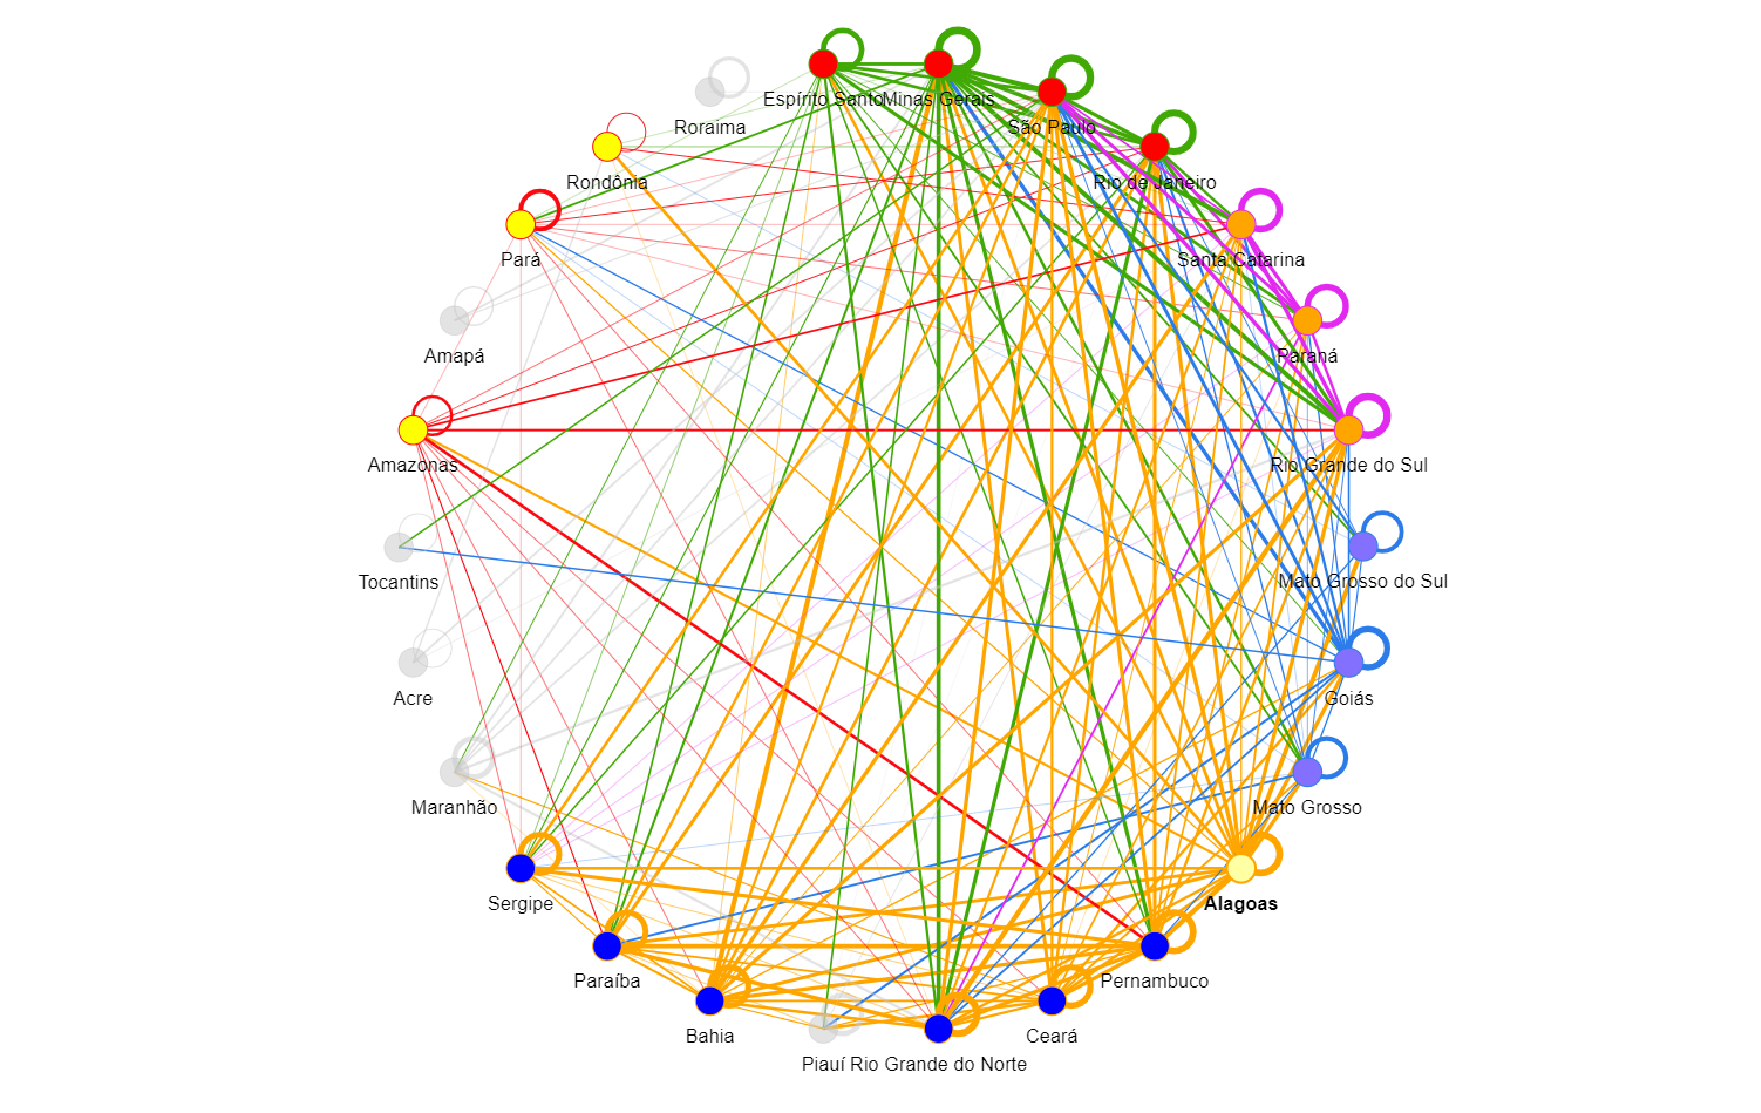
\includegraphics[scale=0.6]{Imagens/rede-al-2017.pdf}
	\caption{Rede de Coautoria da Universidade Federal de Alagoas (\textit{Health Sciences}) - 2017}
	\label{Rede de Coautoria - UF AL 2017}
\end{figure}


%%% ÁREA AGRICULTURAL SCIENCE


\section{\textbf{Agricultural Sciences}}

\subsubsection{Rede de Coautoria das Universidade Federais do Brasil - Área \textit{Agricultural Sciences}}

\subsubsection{Rede de Coautoria Brasil - Vértice Focal Alagoas - Área \textit{Agricultural Sciences}}


\begin{figure}[H]
	\centering
	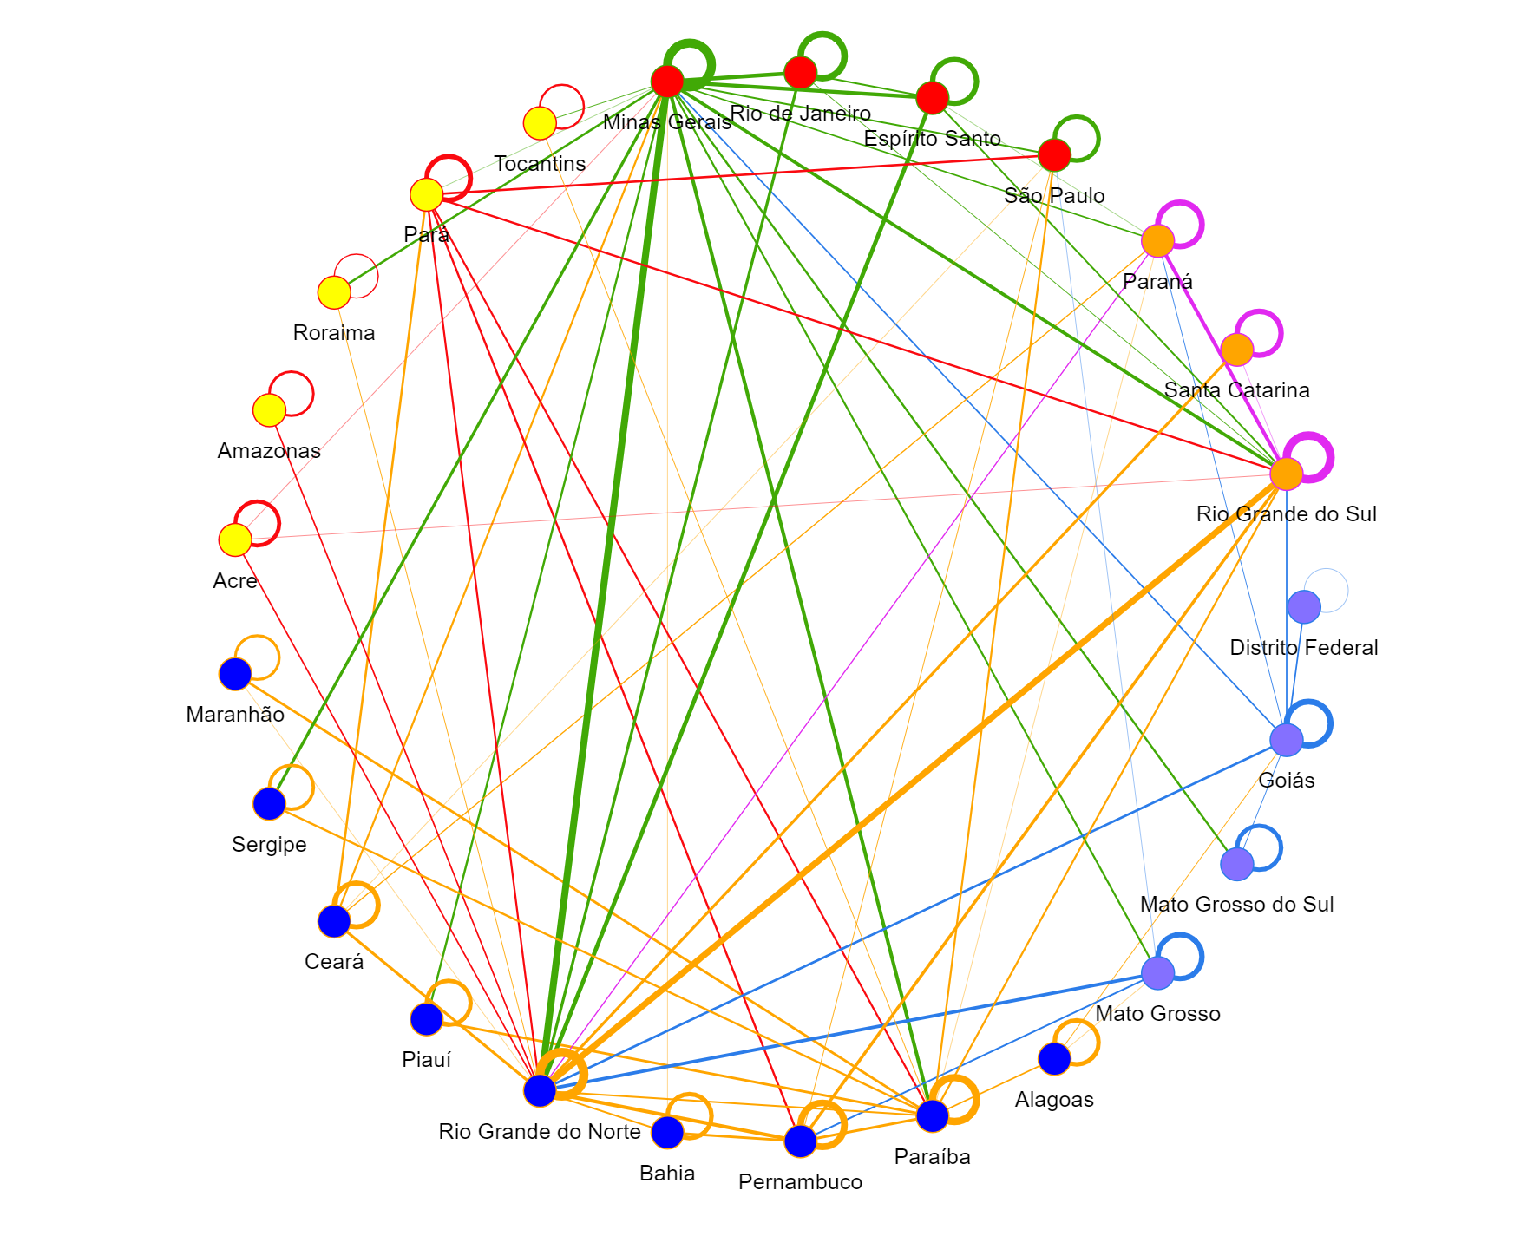
\includegraphics[scale=0.6]{Imagens/rede-agr-br-2008.pdf}
	\caption{Rede de Coautoria das Universidades Federais do Brasil (\textit{Agricultural Sciences}) - 2008}
	\label{Rede de Coautoria - UF AGRI BR 2008}
\end{figure}

\begin{figure}[H]
	\centering
	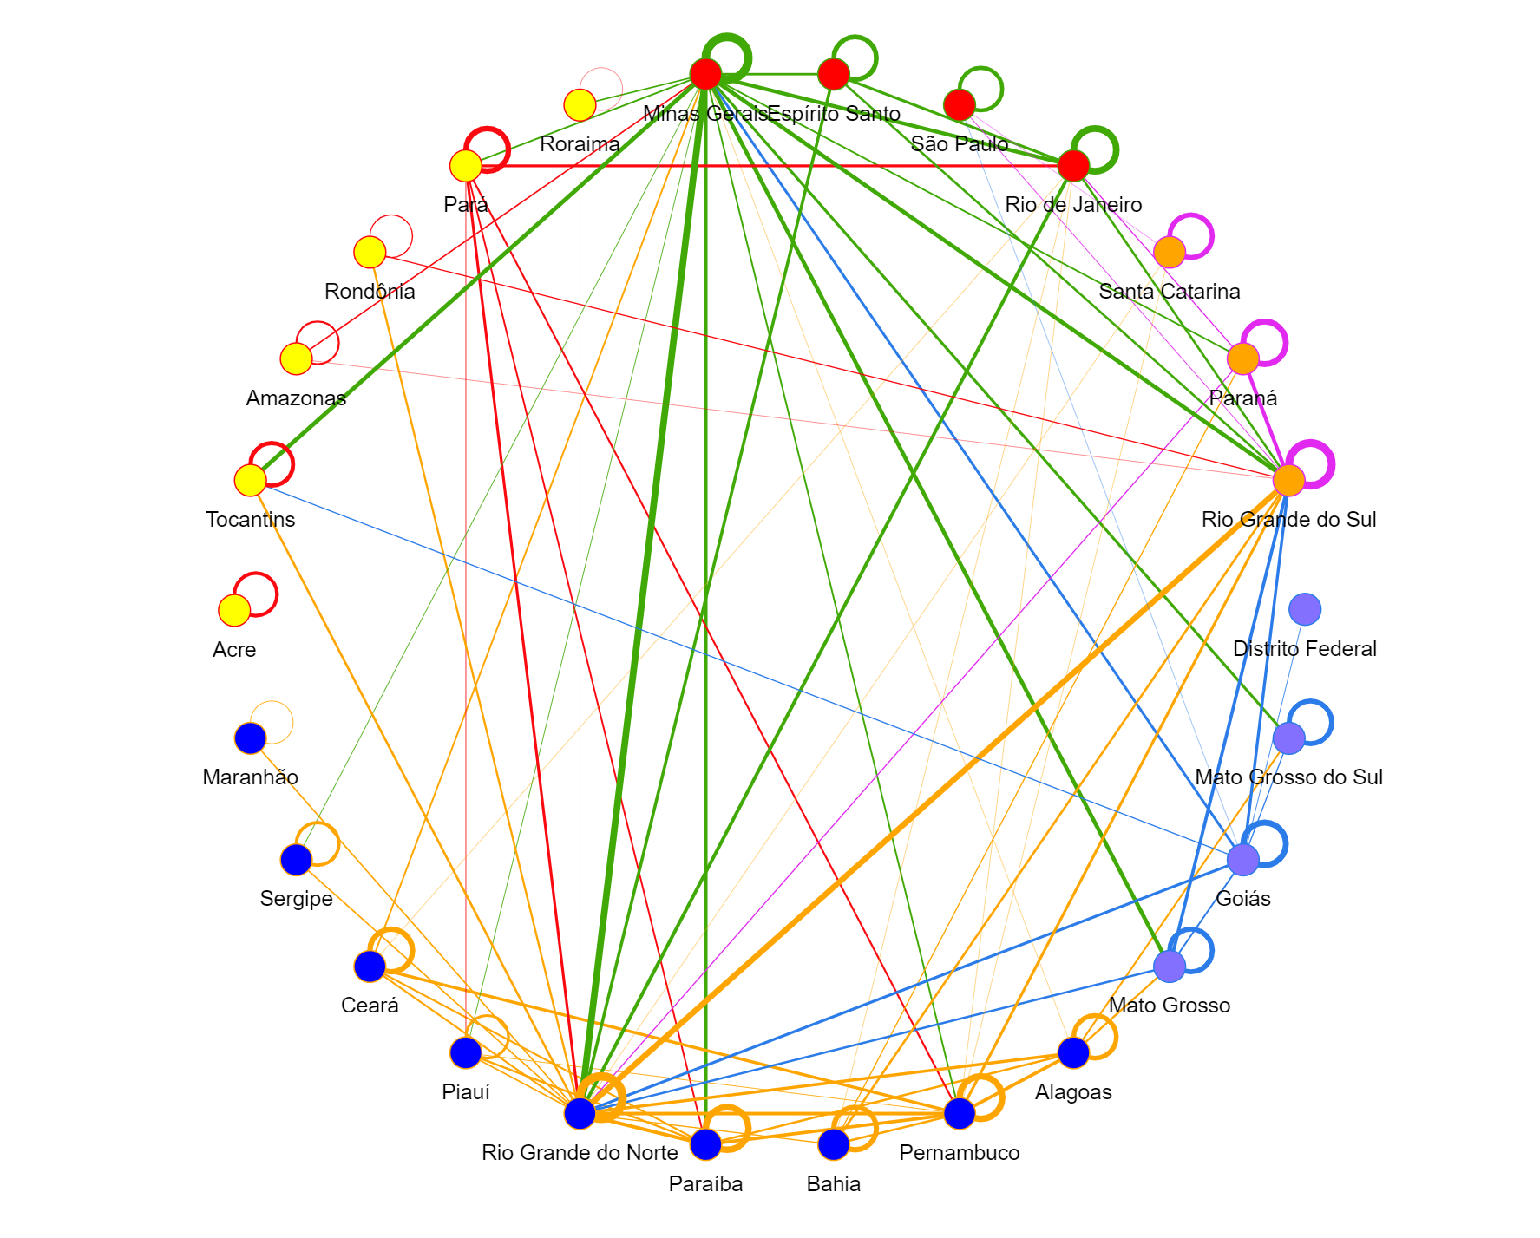
\includegraphics[scale=0.6]{Imagens/rede-agr-br-2009.pdf}
	\caption{Rede de Coautoria das Universidades Federais do Brasil (\textit{Agricultural Sciences}) - 2009}
	\label{Rede de Coautoria - UF AGRI BR 2009}
\end{figure}

\begin{figure}
	\centering
	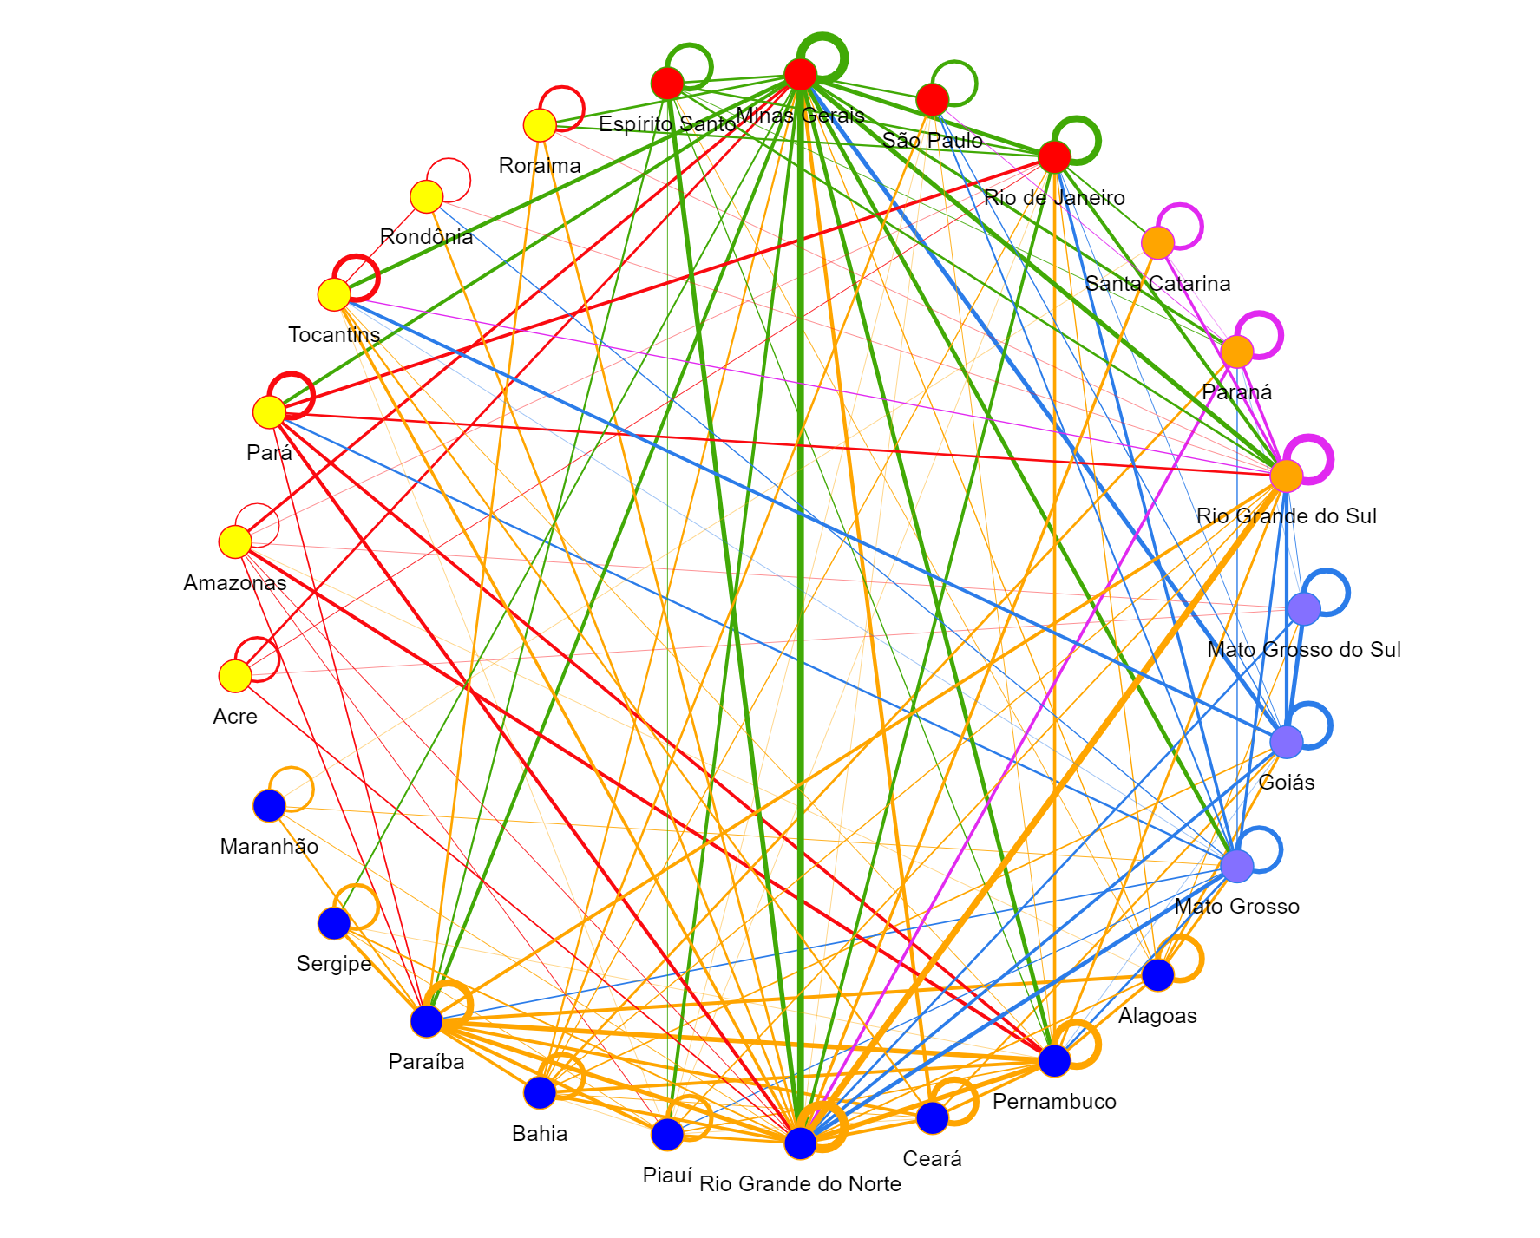
\includegraphics[scale=0.6]{Imagens/rede-agr-br-2010.pdf}
	\caption{Rede de Coautoria das Universidades Federais do Brasil (\textit{Agricultural Sciences}) - 2010}
	\label{Rede de Coautoria - UF AGRI BR 2010}
\end{figure}

\begin{figure}[H]
	\centering
	\includegraphics[scale=0.6]{Imagens/rede-agr-br-2011.pdf}
	\caption{Rede de Coautoria das Universidades Federais do Brasil (\textit{Agricultural Sciences}) - 2011}
	\label{Rede de Coautoria - UF AGRI BR 2011}
\end{figure}


\begin{figure}[H]
	\centering
	\includegraphics[scale=0.6]{Imagens/rede-agr-br-2012.pdf}
	\caption{Rede de Coautoria das Universidades Federais do Brasil (\textit{Agricultural Sciences}) - 2012}
	\label{Rede de Coautoria - UF AGRI BR 2012}
\end{figure}

\begin{figure}[H]
	\centering
	\includegraphics[scale=0.6]{Imagens/rede-agr-br-2013.pdf}
	\caption{Rede de Coautoria das Universidades Federais do Brasil (\textit{Agricultural Sciences}) - 2013}
	\label{Rede de Coautoria - UF AGRI BR 2013}
\end{figure}

\begin{figure}[H]
	\centering
	\includegraphics[scale=0.6]{Imagens/rede-agr-br-2014.pdf}
	\caption{Rede de Coautoria das Universidades Federais do Brasil (\textit{Agricultural Sciences}) - 2014}
	\label{Rede de Coautoria - UF AGRI BR 2014}
\end{figure}


\begin{figure}[H]
	\centering
	\includegraphics[scale=0.6]{Imagens/rede-agr-br-2015.pdf}
	\caption{Rede de Coautoria das Universidades Federais do Brasil (\textit{Agricultural Sciences}) - 2015}
	\label{Rede de Coautoria - UF AGRI BR 2015}
\end{figure}

\begin{figure}[H]
	\centering
	\includegraphics[scale=0.6]{Imagens/rede-agr-br-2016.pdf}
	\caption{Rede de Coautoria das Universidades Federais do Brasil (\textit{Agricultural Sciences}) - 2016}
	\label{Rede de Coautoria - UF AGRI BR 2016}
\end{figure}

\begin{figure}[H]
	\centering
	\includegraphics[scale=0.6]{Imagens/rede-agr-br-2017.pdf}
	\caption{Rede de Coautoria das Universidades Federais do Brasil (\textit{Agricultural Sciences}) - 2017}
	\label{Rede de Coautoria - UF AGRI BR 2017}
\end{figure}

\subsubsection{Rede Alagoas - Área: \textit{Agricultural Sciences}}

\begin{figure}[H]
	\centering
	\includegraphics[scale=0.6]{Imagens/rede-agr-AL-2008.pdf}
	\caption{Rede de Coautoria da Universidade Federal de Alagoas (\textit{Agricultural Sciences}) - 2008}
	\label{Rede de Coautoria - UF AGRI AL 2008}
\end{figure}

\begin{figure}[H]
	\centering
	\includegraphics[scale=0.6]{Imagens/rede-agr-AL-2009.pdf}
	\caption{Rede de Coautoria da Universidade Federal de Alagoas (\textit{Agricultural Sciences}) - 2009}
	\label{Rede de Coautoria - UF AGRI AL 2009}
\end{figure}

\begin{figure}[H]
	\centering
	\includegraphics[scale=0.6]{Imagens/rede-agr-AL-2010.pdf}
	\caption{Rede de Coautoria da Universidade Federal de Alagoas (\textit{Agricultural Sciences}) - 2010}
	\label{Rede de Coautoria - UF AGRI AL 2010}
\end{figure}

\begin{figure}[H]
	\centering
	\includegraphics[scale=0.6]{Imagens/rede-agr-AL-2011.pdf}
	\caption{Rede de Coautoria da Universidade Federal de Alagoas (\textit{Agricultural Sciences}) - 2011}
	\label{Rede de Coautoria - UF AGRI AL 2011}
\end{figure}


\begin{figure}[H]
	\centering
	\includegraphics[scale=0.6]{Imagens/rede-agr-AL-2012.pdf}
	\caption{Rede de Coautoria da Universidade Federal de Alagoas (\textit{Agricultural Sciences}) - 2012}
	\label{Rede de Coautoria - UF AGRI AL 2012}
\end{figure}

\begin{figure}[H]
	\centering
	\includegraphics[scale=0.6]{Imagens/rede-agr-AL-2013.pdf}
	\caption{Rede de Coautoria da Universidade Federal de Alagoas (\textit{Agricultural Sciences}) - 2013}
	\label{Rede de Coautoria - UF AGRI AL 2013}
\end{figure}

\begin{figure}[H]
	\centering
	\includegraphics[scale=0.6]{Imagens/rede-agr-AL-2014.pdf}
	\caption{Rede de Coautoria da Universidade Federal de Alagoas (\textit{Agricultural Sciences}) - 2014}
	\label{Rede de Coautoria - UF AGRI AL 2014}
\end{figure}


\begin{figure}[H]
	\centering
	\includegraphics[scale=0.6]{Imagens/rede-agr-AL-2015.pdf}
	\caption{Rede de Coautoria da Universidade Federal de Alagoas (\textit{Agricultural Sciences}) - 2015}
	\label{Rede de Coautoria - UF AGRI AL 2015}
\end{figure}

\begin{figure}[H]
	\centering
	\includegraphics[scale=0.6]{Imagens/rede-agr-AL-2016.pdf}
	\caption{Rede de Coautoria da Universidade Federal de Alagoas (\textit{Agricultural Sciences}) - 2016}
	\label{Rede de Coautoria - UF AGRI AL 2016}
\end{figure}

\begin{figure}[H]
	\centering
	\includegraphics[scale=0.6]{Imagens/rede-agr-AL-2017.pdf}
	\caption{Rede de Coautoria das Universidades Federais do Brasil (\textit{Agricultural Sciences}) - 2017}
	\label{Rede de Coautoria - UF AGRI AL 2017}
\end{figure}

%%% ÁREA EXACT AND EARTH SCIENCES

\section{\textbf{Exact and Earth Sciences}}

\subsubsection{Rede de Coautoria das Universidade Federais do Brasil - Área \textit{Exact and Earth Sciences}}


\begin{figure}[H]
	\centering
	\includegraphics[scale=0.6]{Imagens/rede-exact-br-2008.pdf}
	\caption{Rede de Coautoria das Universidades Federais do Brasil (\textit{Exact and Earth Sciences}) - 2008}
	\label{Rede de Coautoria - UF EXACT BR 2008}
\end{figure}

\begin{figure}[H]
	\centering
	\includegraphics[scale=0.6]{Imagens/rede-exact-br-2009.pdf}
	\caption{Rede de Coautoria das Universidades Federais do Brasil (\textit{Exact and Earth Sciences}) - 2009}
	\label{Rede de Coautoria - UF EXACT BR 2009}
\end{figure}

\begin{figure}[H]
	\centering
	\includegraphics[scale=0.6]{Imagens/rede-exact-br-2010.pdf}
	\caption{Rede de Coautoria das Universidades Federais do Brasil (\textit{Exact and Earth Sciences}) - 2010}
	\label{Rede de Coautoria - UF EXACT BR 2010}
\end{figure}

\begin{figure}[H]
	\centering
	\includegraphics[scale=0.6]{Imagens/rede-exact-br-2011.pdf}
	\caption{Rede de Coautoria das Universidades Federais do Brasil (\textit{Exact and Earth Sciences}) - 2011}
	\label{Rede de Coautoria - UF EXACT BR 2011}
\end{figure}


\begin{figure}[H]
	\centering
	\includegraphics[scale=0.6]{Imagens/rede-exact-br-2012.pdf}
	\caption{Rede de Coautoria das Universidades Federais do Brasil (\textit{Exact and Earth Sciences}) - 2012}
	\label{Rede de Coautoria - UF EXACT BR 2012}
\end{figure}

\begin{figure}[H]
	\centering
	\includegraphics[scale=0.6]{Imagens/rede-exact-br-2013.pdf}
	\caption{Rede de Coautoria das Universidades Federais do Brasil (\textit{Exact and Earth Sciences}) - 2013}
	\label{Rede de Coautoria - UF EXACT BR 2013}
\end{figure}

\begin{figure}[H]
	\centering
	\includegraphics[scale=0.6]{Imagens/rede-exact-br-2014.pdf}
	\caption{Rede de Coautoria das Universidades Federais do Brasil (\textit{Exact and Earth Sciences}) - 2014}
	\label{Rede de Coautoria - UF EXACT BR 2014}
\end{figure}


\begin{figure}[H]
	\centering
	\includegraphics[scale=0.6]{Imagens/rede-exact-br-2015.pdf}
	\caption{Rede de Coautoria das Universidades Federais do Brasil (\textit{Exact and Earth Sciences}) - 2015}
	\label{Rede de Coautoria - UF EXACT BR 2015}
\end{figure}

\begin{figure}[H]
	\centering
	\includegraphics[scale=0.6]{Imagens/rede-exact-br-2016.pdf}
	\caption{Rede de Coautoria das Universidades Federais do Brasil (\textit{Exact and Earth Sciences}) - 2016}
	\label{Rede de Coautoria - UF EXACT BR 2016}
\end{figure}

\begin{figure}[H]
	\centering
	\includegraphics[scale=0.6]{Imagens/rede-exact-br-2017.pdf}
	\caption{Rede de Coautoria das Universidades Federais do Brasil (\textit{Exact and Earth Sciences}) - 2017}
	\label{Rede de Coautoria - UF EXACT BR 2017}
\end{figure}


\subsubsection{Rede de Coautoria Brasil - Vértice Focal Alagoas - Área \textit{Exact and Earth Sciences}}

\begin{figure}[H]
	\centering
	\includegraphics[scale=0.6]{Imagens/rede-exact-AL-2008.pdf}
	\caption{Rede de Coautoria das Universidades Federais do Brasil (\textit{Exact and Earth Sciences}) - 2008}
	\label{Rede de Coautoria - UF EXACT AL 2008}
\end{figure}

\begin{figure}[H]
	\centering
	\includegraphics[scale=0.6]{Imagens/rede-exact-AL-2009.pdf}
	\caption{Rede de Coautoria das Universidades Federais do Brasil (\textit{Exact and Earth Sciences}) - 2009}
	\label{Rede de Coautoria - UF EXACT AL 2009}
\end{figure}

\begin{figure}[H]
	\centering
	\includegraphics[scale=0.6]{Imagens/rede-exact-AL-2010.pdf}
	\caption{Rede de Coautoria das Universidades Federais do Brasil (\textit{Exact and Earth Sciences}) - 2010}
	\label{Rede de Coautoria - UF EXACT AL 2010}
\end{figure}

\begin{figure}[H]
	\centering
	\includegraphics[scale=0.6]{Imagens/rede-exact-AL-2011.pdf}
	\caption{Rede de Coautoria das Universidades Federais do Brasil (\textit{Exact and Earth Sciences}) - 2011}
	\label{Rede de Coautoria - UF EXACT AL 2012}
\end{figure}


\begin{figure}[H]
	\centering
	\includegraphics[scale=0.6]{Imagens/rede-exact-AL-2012.pdf}
	\caption{Rede de Coautoria das Universidades Federais do Brasil (\textit{Exact and Earth Sciences}) - 2012}
	\label{Rede de Coautoria - UF EXACT AL 2012}
\end{figure}

\begin{figure}[H]
	\centering
	\includegraphics[scale=0.6]{Imagens/rede-exact-AL-2013.pdf}
	\caption{Rede de Coautoria das Universidades Federais do Brasil (\textit{Exact and Earth Sciences}) - 2013}
	\label{Rede de Coautoria - UF EXACT AL 2013}
\end{figure}

\begin{figure}[H]
	\centering
	\includegraphics[scale=0.6]{Imagens/rede-exact-AL-2014.pdf}
	\caption{Rede de Coautoria das Universidades Federais do Brasil (\textit{Exact and Earth Sciences}) - 2014}
	\label{Rede de Coautoria - UF EXACT AL 2014}
\end{figure}


\begin{figure}[H]
	\centering
	\includegraphics[scale=0.6]{Imagens/rede-exact-AL-2015.pdf}
	\caption{Rede de Coautoria das Universidades Federais do Brasil (\textit{Exact and Earth Sciences}) - 2015}
	\label{Rede de Coautoria - UF EXACT AL 2015}
\end{figure}

\begin{figure}[H]
	\centering
	\includegraphics[scale=0.6]{Imagens/rede-exact-AL-2016.pdf}
	\caption{Rede de Coautoria das Universidades Federais do Brasil (\textit{Exact and Earth Sciences}) - 2016}
	\label{Rede de Coautoria - UF EXACT AL 2016}
\end{figure}

\begin{figure}[H]
	\centering
	\includegraphics[scale=0.6]{Imagens/rede-exact-AL-2017.pdf}
	\caption{Rede de Coautoria das Universidades Federais do Brasil (\textit{Exact and Earth Sciences}) - 2017}
	\label{Rede de Coautoria - UF EXACT AL 2017}
\end{figure}

%======================================================%
%============= REFERÊNCIAS BIBLIOGRÁFICAS =============%
%======================================================%
\begin{raggedright}
%\bibliographystyle{agsm_url}
\bibliographystyle{agsm}
\renewcommand{\bibsection}{
\chapter*{\vspace{-3cm}\centering \Large \textsc{Referências Bibliográficas}}
\addcontentsline{toc}{chapter}{Referências Bibliográficas}
}
\lhead{\textsc{Referências Bibliográficas}}
\bibliography{./Bibliography/Ref}
\newpage\lhead{\rightmark}
\end{raggedright}


%======================================================%

\chapter*{}
\vfill
\singlespacing
\thispagestyle{empty}
\begin{center}
Este trabalho foi redigido em {\large \LaTeX}\ utilizando uma modificação do estilo \textsf{IC-UFAL}.
As referências bibliográficas foram preparadas no \textsf{Mendeley} e administradas pelo {\large\BibTeX}\ com o estilo \textsf{LaCCAN}.
O texto utiliza fonte \NomeFonte\ e os elementos matemáticos a família tipográfica \NomeFonteMat, ambas em corpo de 12 pontos.
% A numeração dos capítulos segue com a família tipográfica \NomeFonteCap.\\ 
% \vspace{.5cm}
% \includegraphics[width=.2\textwidth]{../figs/gondor_invertida}
\end{center}

\end{document}